
\subsection{Charge flip leptons}
\label{sec:bkg_chflips}

The lepton charge mis-measurement commonly referred to as ``charge flip'' background, 
is an experimental background strongly associated to analyses relying on same-sign leptons final states. 
In those events, the electric charge of one of the two leptons forming an opposite-sign (OS) pair, coming from an abundant SM process ($pp\to Z,\,t\bar{t},\,W^+W^-$\ldots), is mis-identified leading to a much rarer SS pair event. 
The most frequent origin of this mis-identification is the following: 
when an electron goes through a medium (in this case, the ATLAS inner detector), it can produce a hard photon by Bremsstrahlung radiation which can then convert in an $e^+e^-$ pair. If the converted electron with the largest $\pt$ has an opposite charge compared to the original electron (the one that emits the hard photon), wrong sign will be assigned to the initial electron track, leading to a charge-flip event. Errors on the track charge assignment itself may occur as well, but they are much rarer. 

We rely on a purely data-driven method to estimate yields of events with charge flipped electrons. 
Assuming one knows the electron charge flip rates $\xi(\eta,p_T)$, a simple way to predict these yields is to select 
events with pairs of opposite-sign leptons in data and assign them a weight: 

\begin{align}
w = \xi\left(\eta^{1},p_T^{1}\right)\left[1-\xi\left(\eta^{2},p_T^{2}\right)\right] 
+ \xi\left(\eta^{2},p_T^{2}\right)\left[1-\xi\left(\eta^{1},p_T^{1}\right)\right] 
\end{align}
where $\xi=0$ for muons. 

The advantages of this method are a good statistical precision since the charge flip rate is quite small, 
and the lack of dependency on the simulation and related uncertainties. 
Obviously, it requires a precise measurement of the rates, which is described in the next paragraph. 
A slight inconvenient is that the reconstructed electron energy, for charge flipped electrons, 
tends to be negatively biased (too low by a few~\GeV), because of the hard Bremsstrahlung at the origin of the charge flip. 
Simply reweighting electrons from opposite-sign lepton pairs therefore does not predict correctly the charge-flip background shape 
for variables strongly dependending on the electron momentum. 
But we do not rely on such discriminant variables, therefore we simply neglect this effect for the moment. 

In order to correctly define this background and to estimate the number of charge flip events in our signal regions, one has to measure the rate (probability) of electron charge mis-measurement. The probability of mis-identifying a muon was found to be negligible, at least for the $\pt$ range considered in this analysis. 
This section is organized as follows: first the procedure to extract the charge flip rate is explained and then, 
the charge flip rates measured with the 2015 dataset are presented. 
A dedicated study of the charge flip rates in different MC productions (MC12, DC14, MC15) can be found in Appendix~\ref{app:flips}.


\par{\bf Measurement of the charge flip rates}

The charge flip rate is extracted with a data-driven technique using a likelihood fit, within a $Z$ boson control sample defined by requiring a pair of SS or OS electrons with invariant mass between 75 and 100 GeV. Since the amount of material the electrons pass through is related to $\eta$, the probability of mis-measuring the charge will depend on $\eta$. Moreover, since the inner detector track curvature is used to measured the charge, the charge flip rate will also be dependent on the electron $\pt$.  
The extraction of charge flip rates will then be performed for a specific ($\eta, \pt$) binning in order to take into account those effects. In the following, the total number of bins is defined as the product of number of $\eta$ bins and number of $\pt$ bins: \# (total bins) = \# ($\eta$ bins) $\times$ \# ($\pt$ bins). The notation "bin $A$", where $A$ can take any values between 0 and \# (total bins), refer to one specific combination of ($\eta,\pt$) bins.

The likelihood fit used to measure the charge flip rate maximizes the function

\begin{equation}
\label{eq:llh}
L = \prod_{I, J} L_{\epsilon(I),\epsilon(J)},
\end{equation}

where $L_{\epsilon(I),\epsilon(J)}$ is the following Poisson distribution:

\begin{equation}
\label{eq:pois}
L_{\epsilon(I),\epsilon(J)} = P(N_{SS}^{obs} | \epsilon(I), \epsilon(J)) = \frac{(N_{SS}^{exp})^{N_{SS}^{obs}} e^{-N_{SS}^{exp}} } {N_{SS}^{obs} !}.
\end{equation}

At this point, we set that the leading electron coming from $Z$ boson falls into bin $I$ while the subleading electron falls into bin $J$. In eq. \ref{eq:llh} and \ref{eq:pois}, $\epsilon(I)$ ($\epsilon(J)$) is then the probability of mis-measuring the charge of an electron that falls into bin $I$ ($J$). The variable $N_{SS}^{obs}$ stands for the observed number of SS events while $N_{SS}^{exp}$ is the expected number of SS events and is defined as:

\begin{equation}
\label{eq:nss}
N_{SS}^{exp} = N ( (1-\epsilon(I))\epsilon(J) + (1-\epsilon(J))\epsilon(I) ),
\end{equation}

with $N$ the total number of events. 
This likelihood fit method is performed with a {\tt TMinuit} routine 
and returns a charge flip rate values for each different ($\eta,\pt$) bin 
as well as the associate statistical errors.

\par{\bf Charge flip rate results}

The comparison of charge flip rates extracted from Monte Carlo simulation and data is important in order to validate our choice of control region. 
In this section, the first results of charge flip rates measured in data are compared to the rates from an MC15 $Z\to e^+e^-$ sample.
To extract the \textit{nominal} charge flip rates, both electrons forming the SS or OS pair must pass the signal selections. 
As explained further in section~\ref{sec:bkg_matrix_method}, the method used to predict the yields of fake leptons requires estimates of the charge flip background 
also for baseline electrons failing the signal requirements. 
A similar methodology is used to extract the charge flip rates for pre-selected (non-signal) electrons 
albeit modified according to the specificities of the measurement (larger background, asymmetry between the definitions of the two selected electrons). 
For this last measurement, the definition of the binning in eq. \ref{eq:llh} to \ref{eq:nss} is different. Instead of referring to the leading and sub-leading electron, $I$ will refer to the bin where the signal electron falls, while $J$ refer to the bin where the non-signal electron falls. Then, $\epsilon(I)$ ($\epsilon (J)$) becomes the probability of mis-measuring the charge of a signal (non-signal) electron that falls into bin $I$ ($J$). In other words, there is no requirement for the leading electron to be neither the signal nor the non-signal electron of the pair.

Figure~\ref{fig:ptsig} shows kinematic $\pt$ distributions, before the background subtraction, 
for nominal measurement on left and loose measurement on right while the $\eta$ distributions are shown on Figure~\ref{fig:etasig}. 
In those plots, the electrons forming an OS (black filled dots for data, blue area for MC) and a SS pair (black circle for data, green area for MC) 
are shown separately and the MC areas are normalized (scaled) to the data luminosity.
% For both Figure~\ref{fig:ptsig} and~\ref{fig:etasig}, the agreement between data and MC is good. 
% -> commented out because it's not tru for loose electrons, because of the background (no mll cut applied in the figure -> large bkg...)
The small discrepancies at low $\pt$ may be due to some Drell-Yan processes that are not considered here 
and to the presence of fake electrons in the loose distributions. The discrepancies in the central region for the loose SS distribution on the right plot of Figure \ref{fig:etasig} can also be attributed to the presence of fake electrons in the sample. 


%------------------------------------------------
\begin{figure}[!htb]
\centering
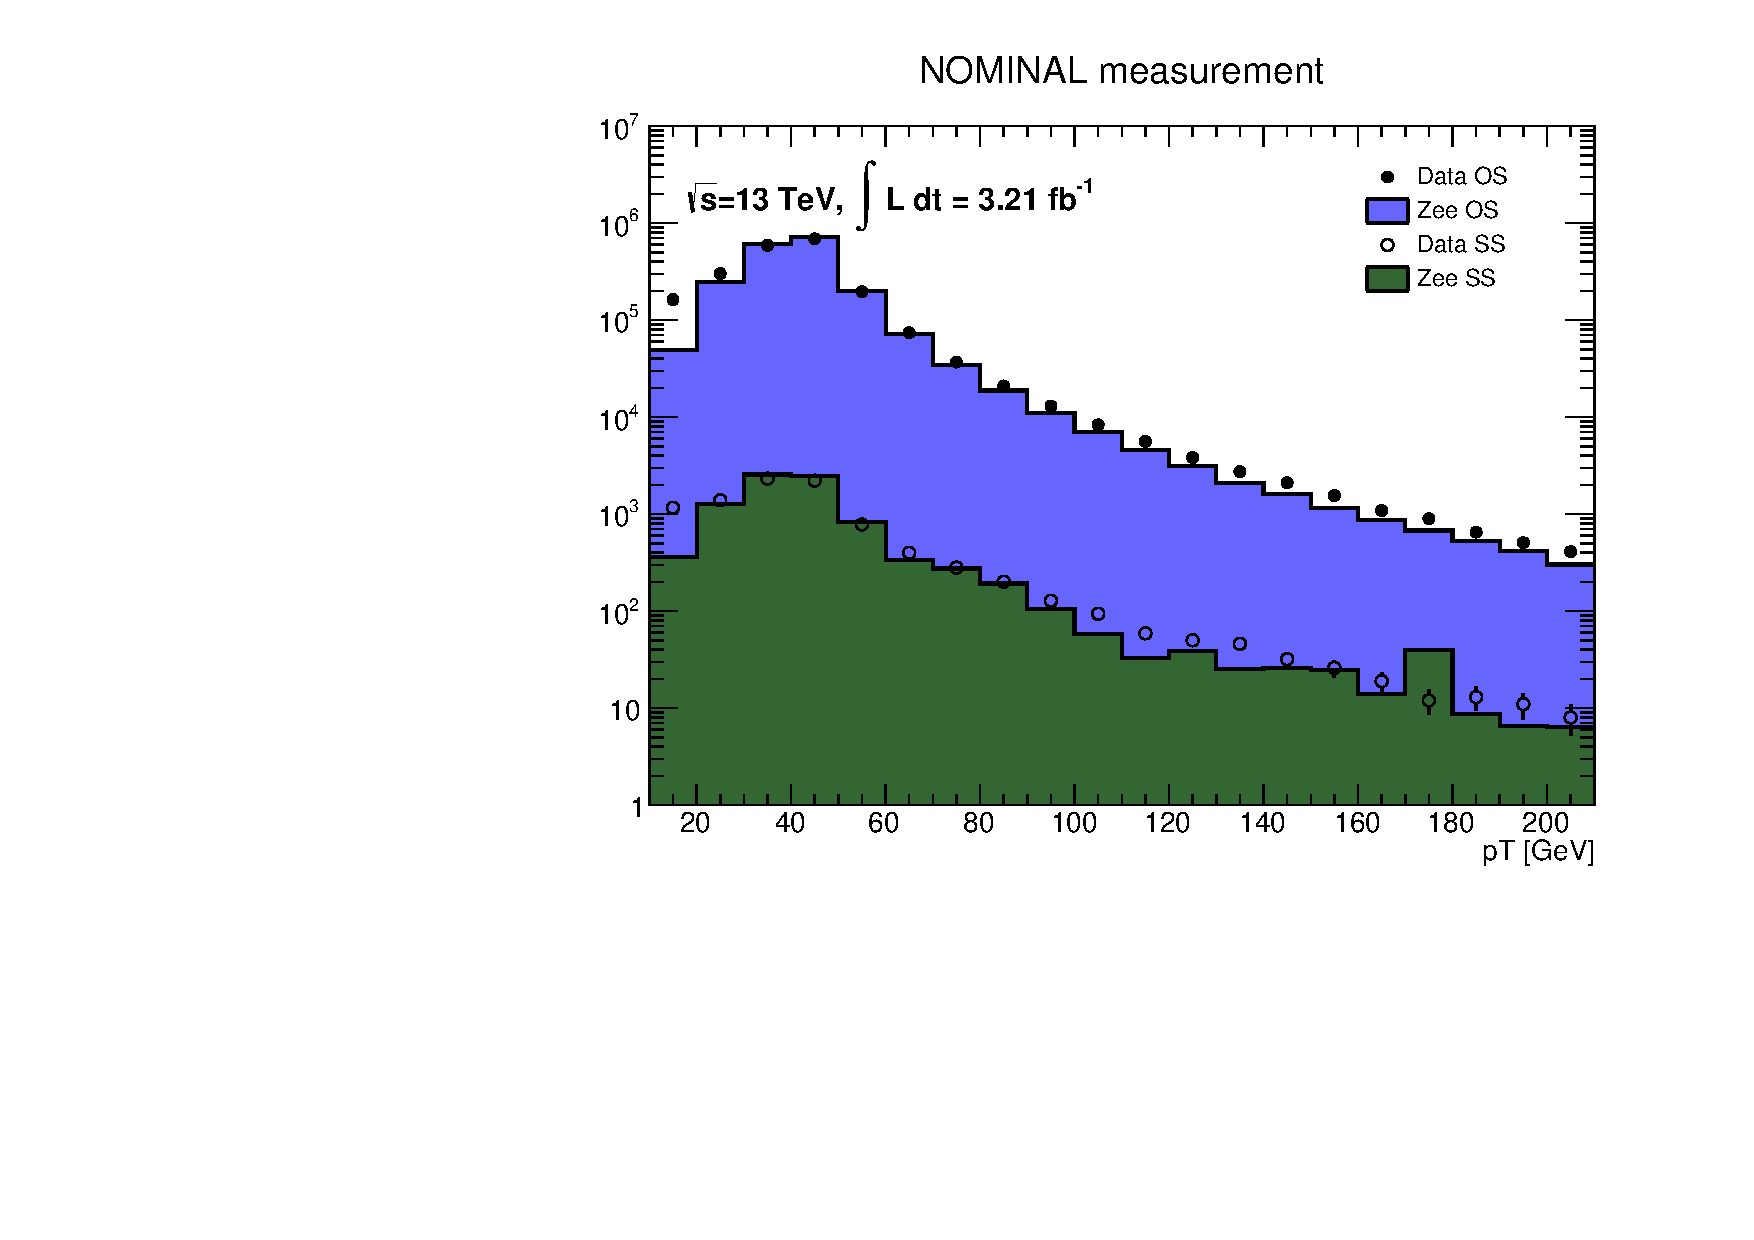
\includegraphics[width=0.4\textwidth]{FIGURES/BKG/chargeFlip/pt_nominal_v28.pdf}
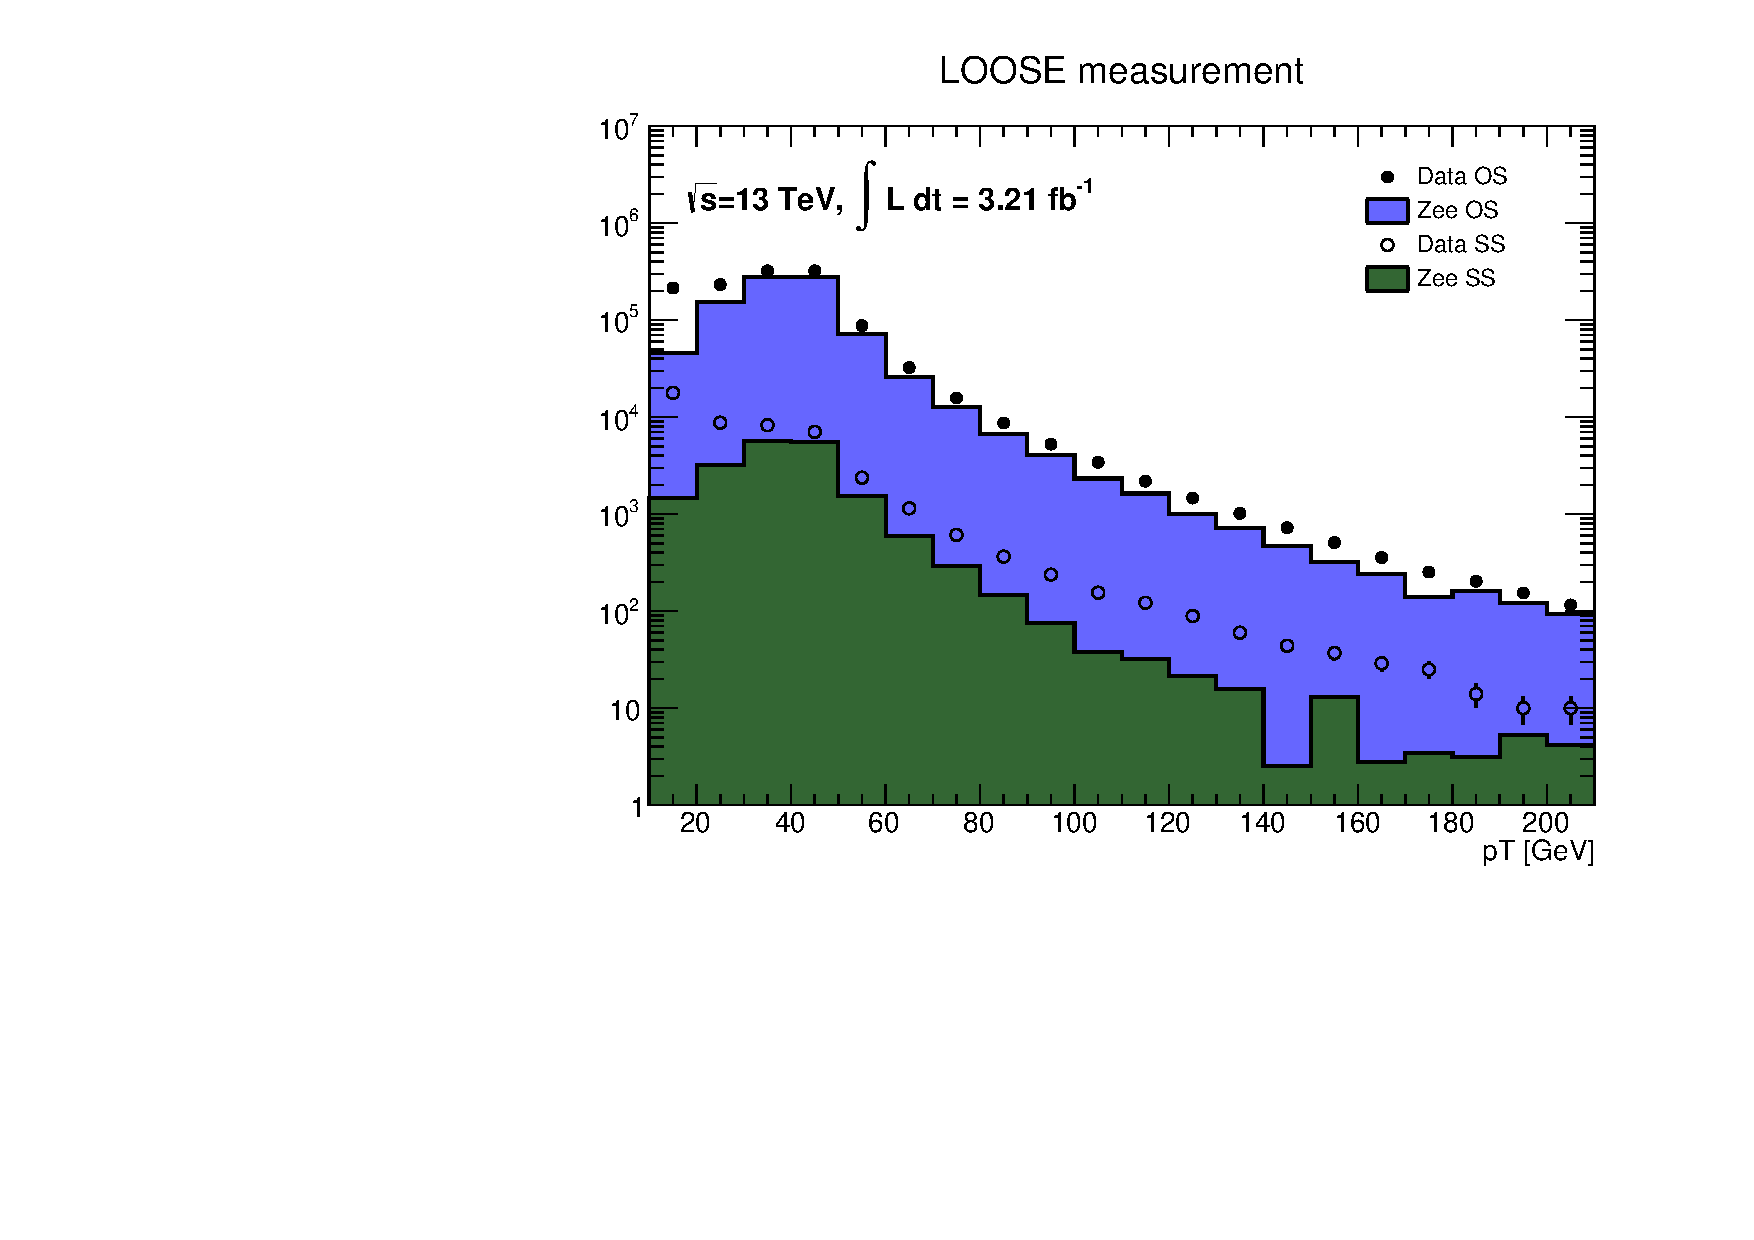
\includegraphics[width=0.4\textwidth]{FIGURES/BKG/chargeFlip/pt_loose_v28.pdf}
\caption{\label{fig:ptsig} $\pt$ distributions for nominal (left) and loose (right) measurements for signal electrons forming an OS pair (filled dots for data, blue area for MC) and a SS pair (empty circles for data, green area for MC). Only statistical uncertainties are shown.}
\end{figure}
%------------------------------------------------

%------------------------------------------------
\begin{figure}[!htb]
\centering
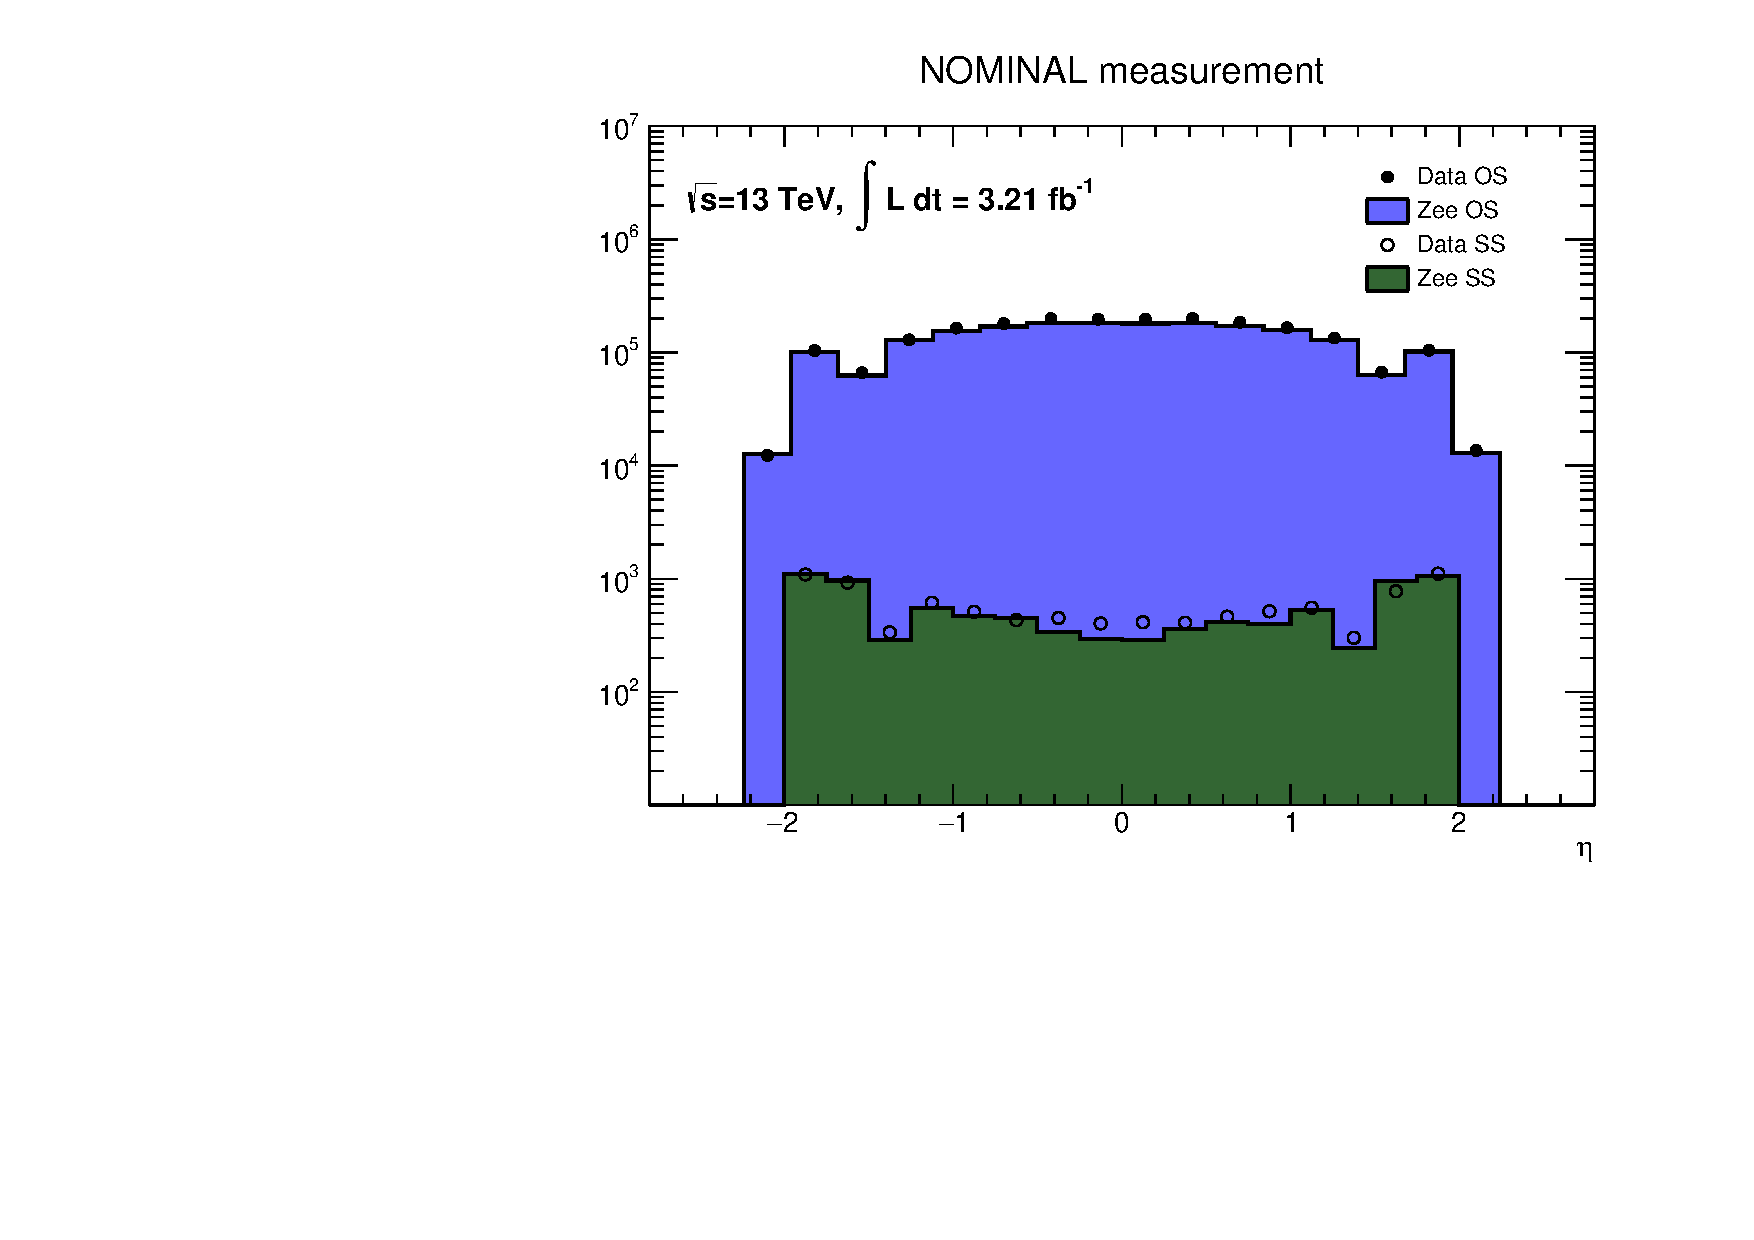
\includegraphics[width=0.4\textwidth]{FIGURES/BKG/chargeFlip/eta_nominal_v28.pdf}
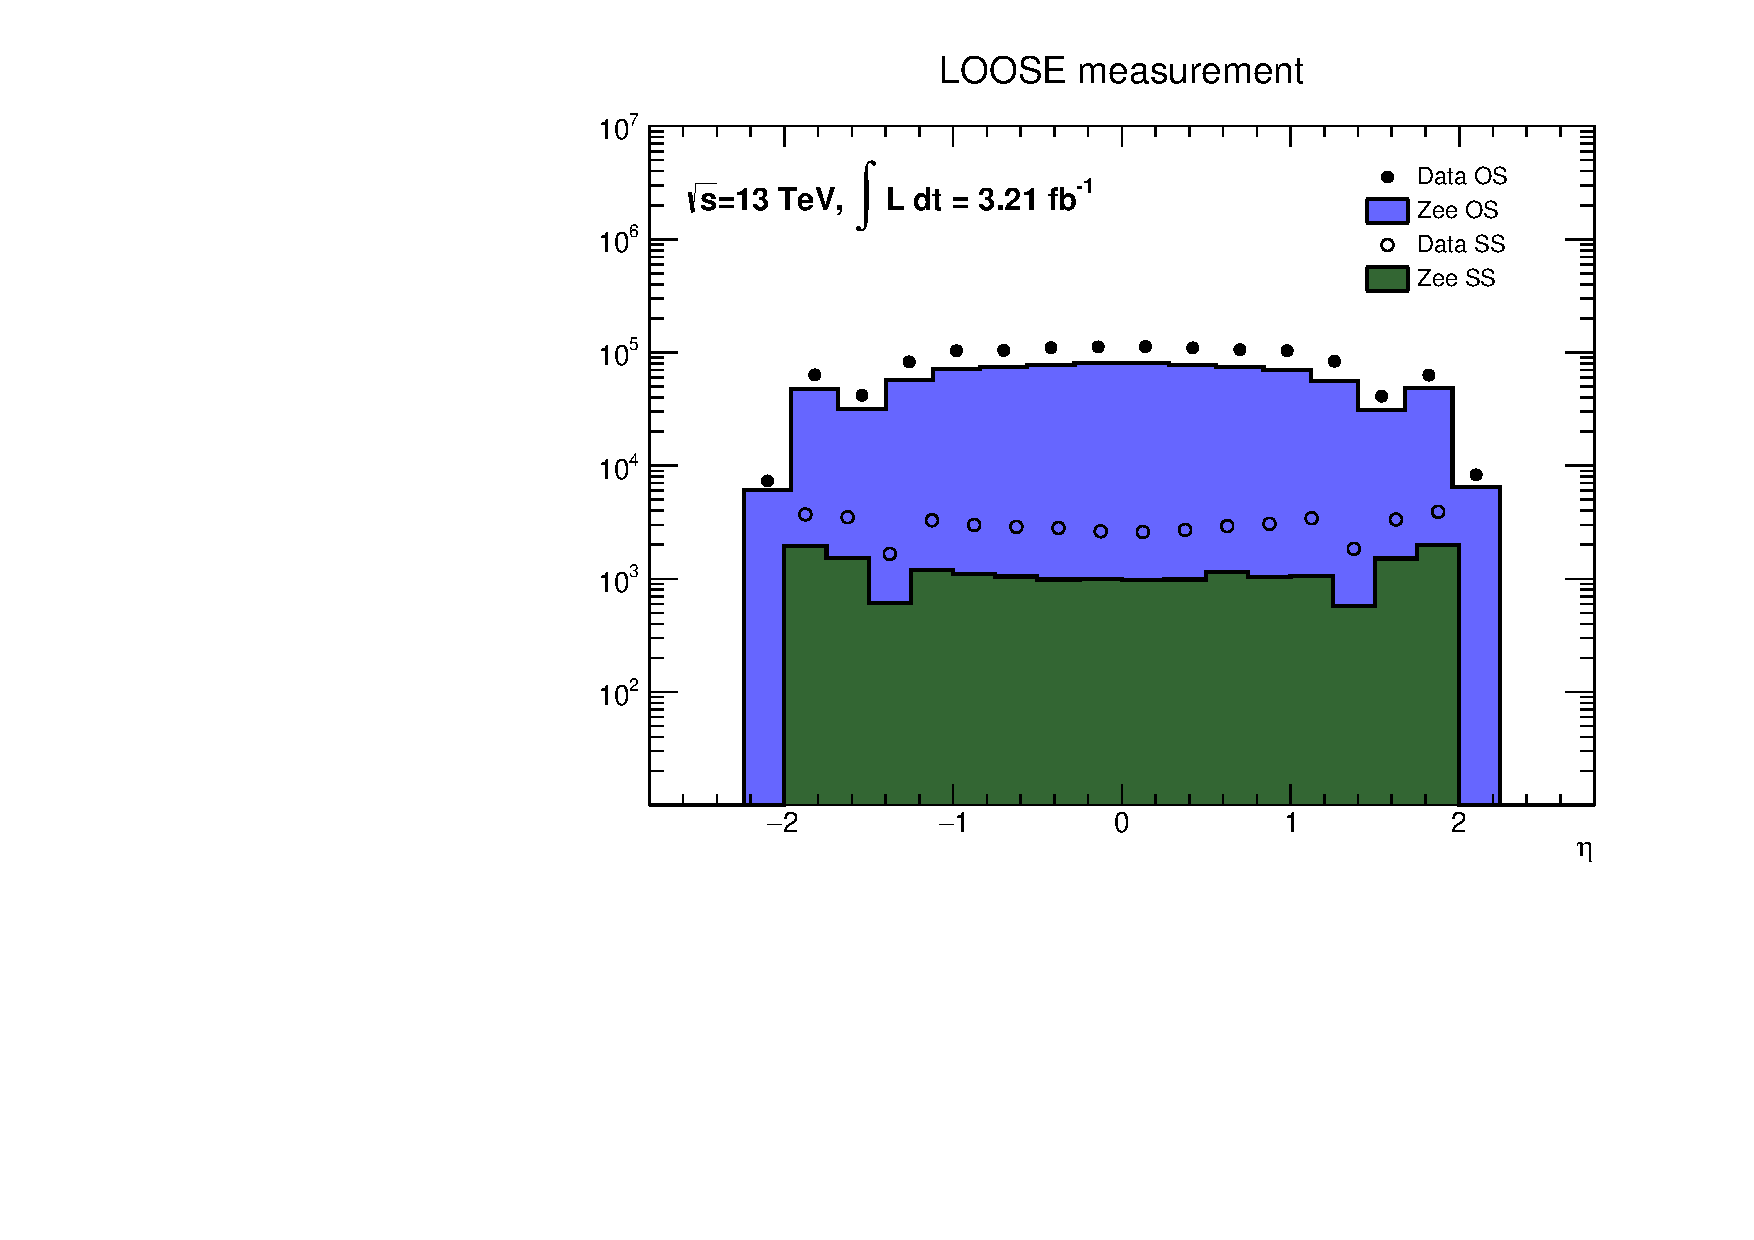
\includegraphics[width=0.4\textwidth]{FIGURES/BKG/chargeFlip/eta_loose_v28.pdf}
\caption{\label{fig:etasig} $\eta$ distributions for nominal (left) and loose (right) measurements for signal electrons forming an OS pair (filled dots for data, blue area for MC) and a SS pair (empty circles for data, green area for MC). Only statistical uncertainties are shown.}
\end{figure}
%------------------------------------------------


The invariant mass of electrons forming the pair is also an important quantity to look at and it is shown on Figure \ref{fig:mll}, where the left plot is the nominal measurement while the right plot correspond to the loose measurement. Again, the electrons forming an OS (black filled dots for data, blue area for MC) and a SS pair (black circle for data, green area for MC) are shown separately and the MC areas are normalized to data luminosity. The background is not subtracted in these plots.

%------------------------------------------------
\begin{figure}[!htb]
\centering
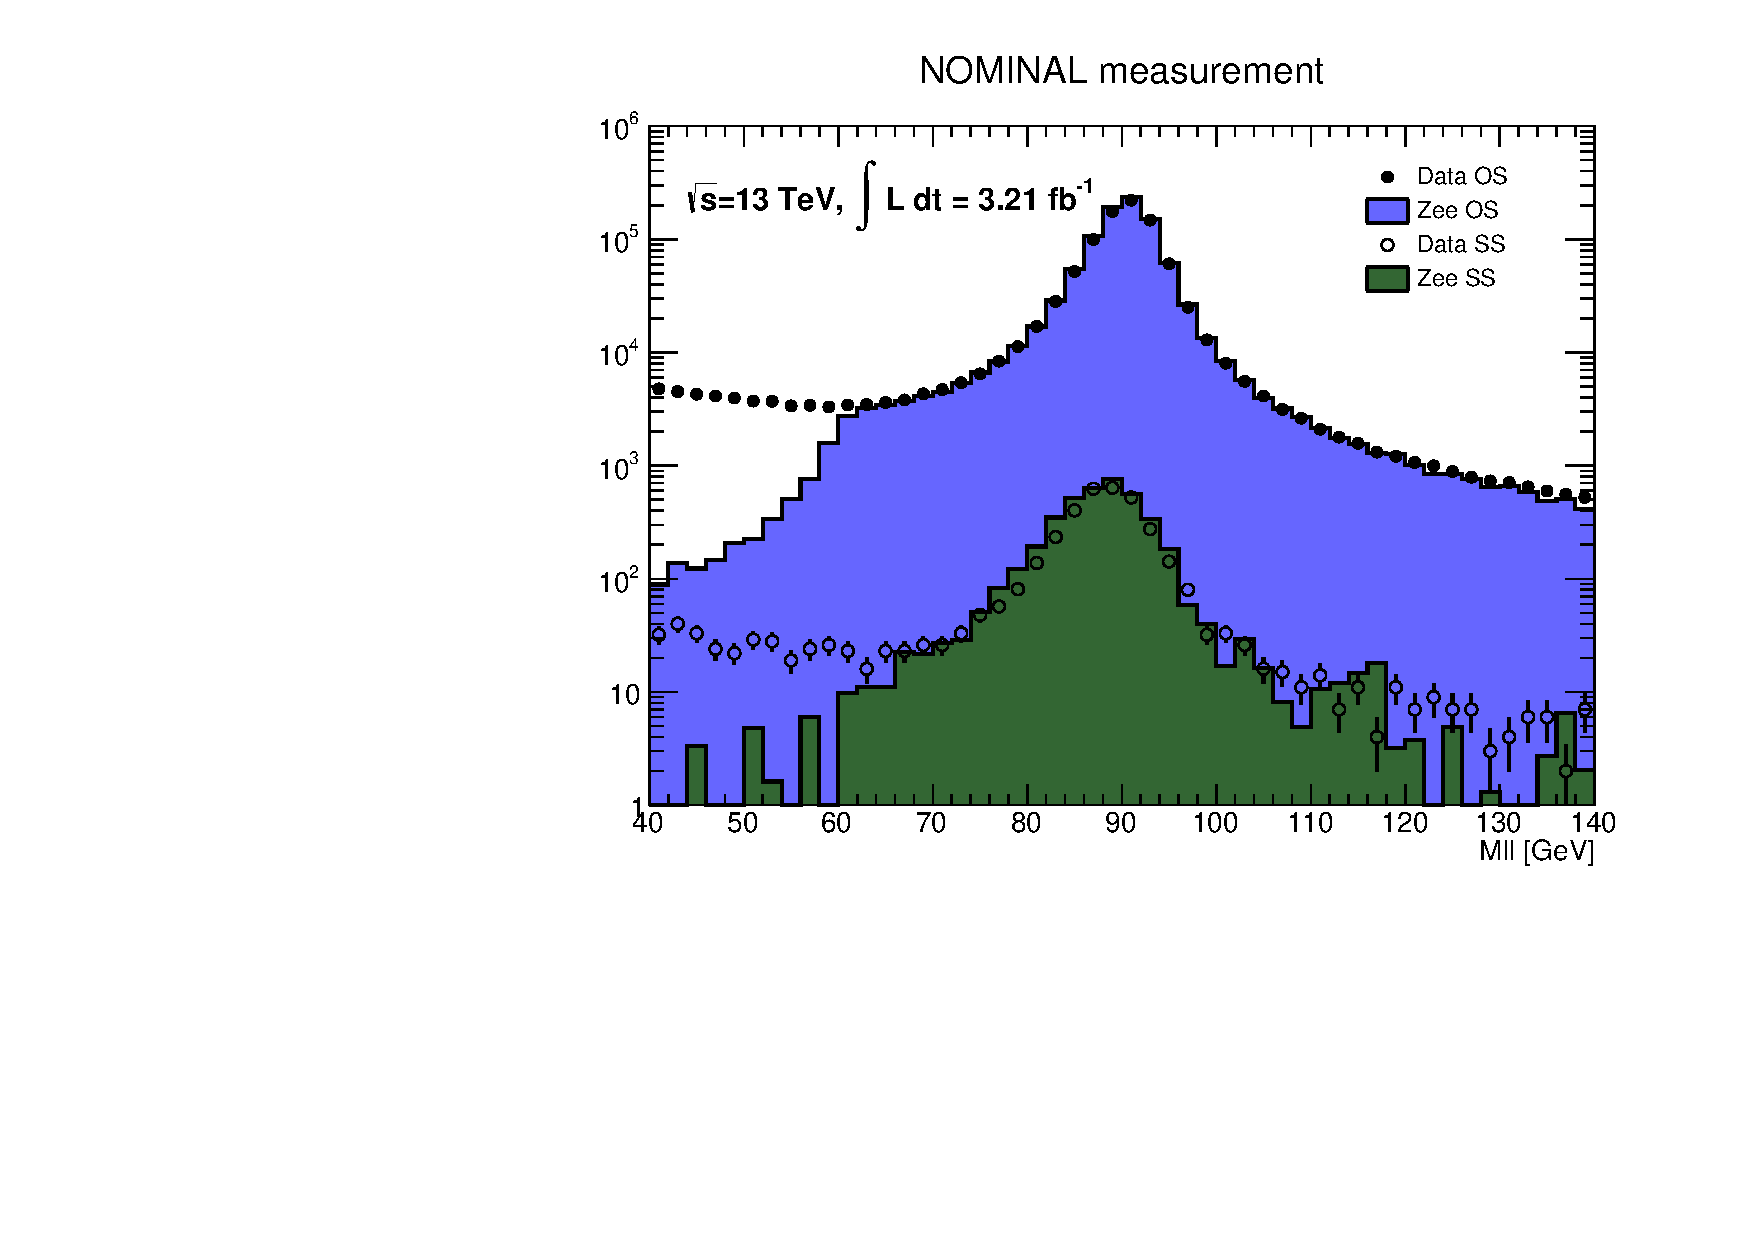
\includegraphics[width=0.4\textwidth]{FIGURES/BKG/chargeFlip/mll_nominal_v28.pdf}
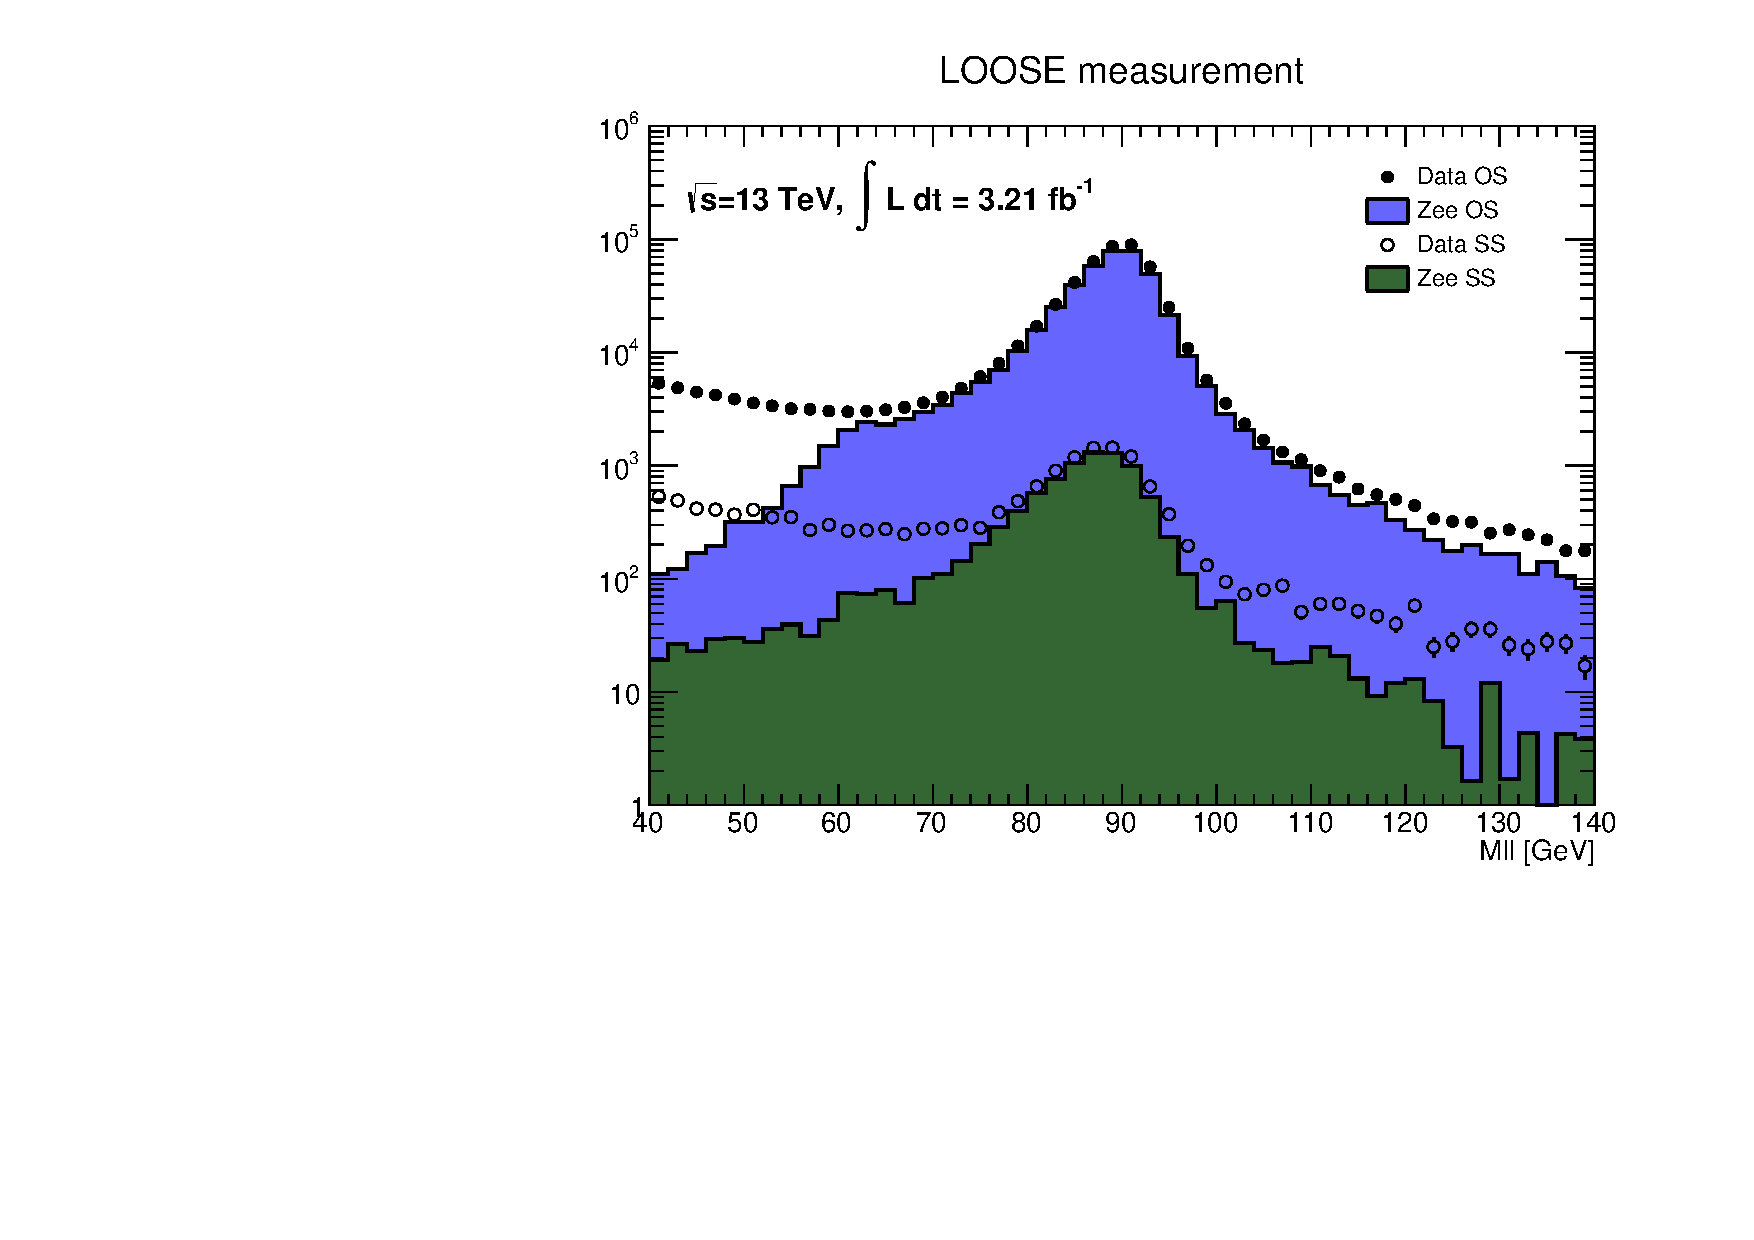
\includegraphics[width=0.4\textwidth]{FIGURES/BKG/chargeFlip/mll_loose_v28.pdf}
\caption{\label{fig:mll} Invariant mass distributions for nominal (left) and loose (right) measurements for signal electrons forming an OS pair (filled dots for data, blue area for MC) and a SS pair (empty circles for data, green area for MC). Only statistical uncertainties are shown.}
\end{figure}
%------------------------------------------------


Despite the small shift toward lower energies in the SS distribution, which is due to the loss of energy during the radiation process, 
one can see that there is a nice agreement between OS and SS pairs within the Z peak. 
Outside the peak, especially at low energy, one can see a large discrepancy in all distributions which comes from the fact 
that $Z\to e^+e^-$ was the only background considered. 
Again Drell-Yan processes and fake electrons (in the loose measurement cases) are the main causes of those differences. 
One can also see on Figure~\ref{fig:mll} that the amount of SS events (empty circles) for loose measurements is greater 
than the number of SS events in the nominal measurement while it is the opposite for the OS distributions (filled dots). 
This is expected since the cuts required to pass the signal requirements were designed to reject as much as possible detector backgrounds such as charge-flip electrons, 
so by requiring that one electron in the pair fails one of these requirements, the effect is clearly to raise the number of SS events and in the same time, 
lower the number of OS events. 
A background subtraction procedure using a side-band method is used to estimate the amount of background events in the measurement region. 
This method uses the number of observed events that fall in the side-band regions, $50<M_{ee}<75$~GeV and $100<M_{ee}<125$~GeV, 
to correct the number of events inside the central-band defined as $75<M_{ee}<100$~GeV. The systematic uncertainties related to those chosen values of central and side bands width are further discussed in the next section.


Finally, the nominal charge flip rates were computed following the procedures explained above for the following set of bins: $\pt$ bins = \{10, 20, 30, 40, 50, 60, 70, 80, 90, 100, 7000\} GeV, $|\eta|$ bins \{0.0, 0.8, 1.37, 2.0\}. In order to reduce the charge mis-identification background, events with an electron within the crack region ($1.37<|\eta|<1.52$) are vetoed as well as events where an electron from the pair has $|\eta|>2.0$. To be sure we got enough statistics in each bin, the number of electrons forming a SS events for the nominal and loose measurements are shown respectively on the top and bottom of Figure~\ref{fig:NSSdata}, where the higher $\pt$ bin contains the overflow. On those plots, one can see that most of the bins contain more than 20 electrons (except some bins at high $\pt$ values), which is enough to produce trustable charge flip rate results. By comparing those two figures, one can also see that the number of SS electrons ($N_{SS}$) is greater in the loose measurement case, but the distribution of $N_{SS}$ over the bins is similar between both measurements.

%-----------------------------------------------
\begin{figure}[!htb]
\centering
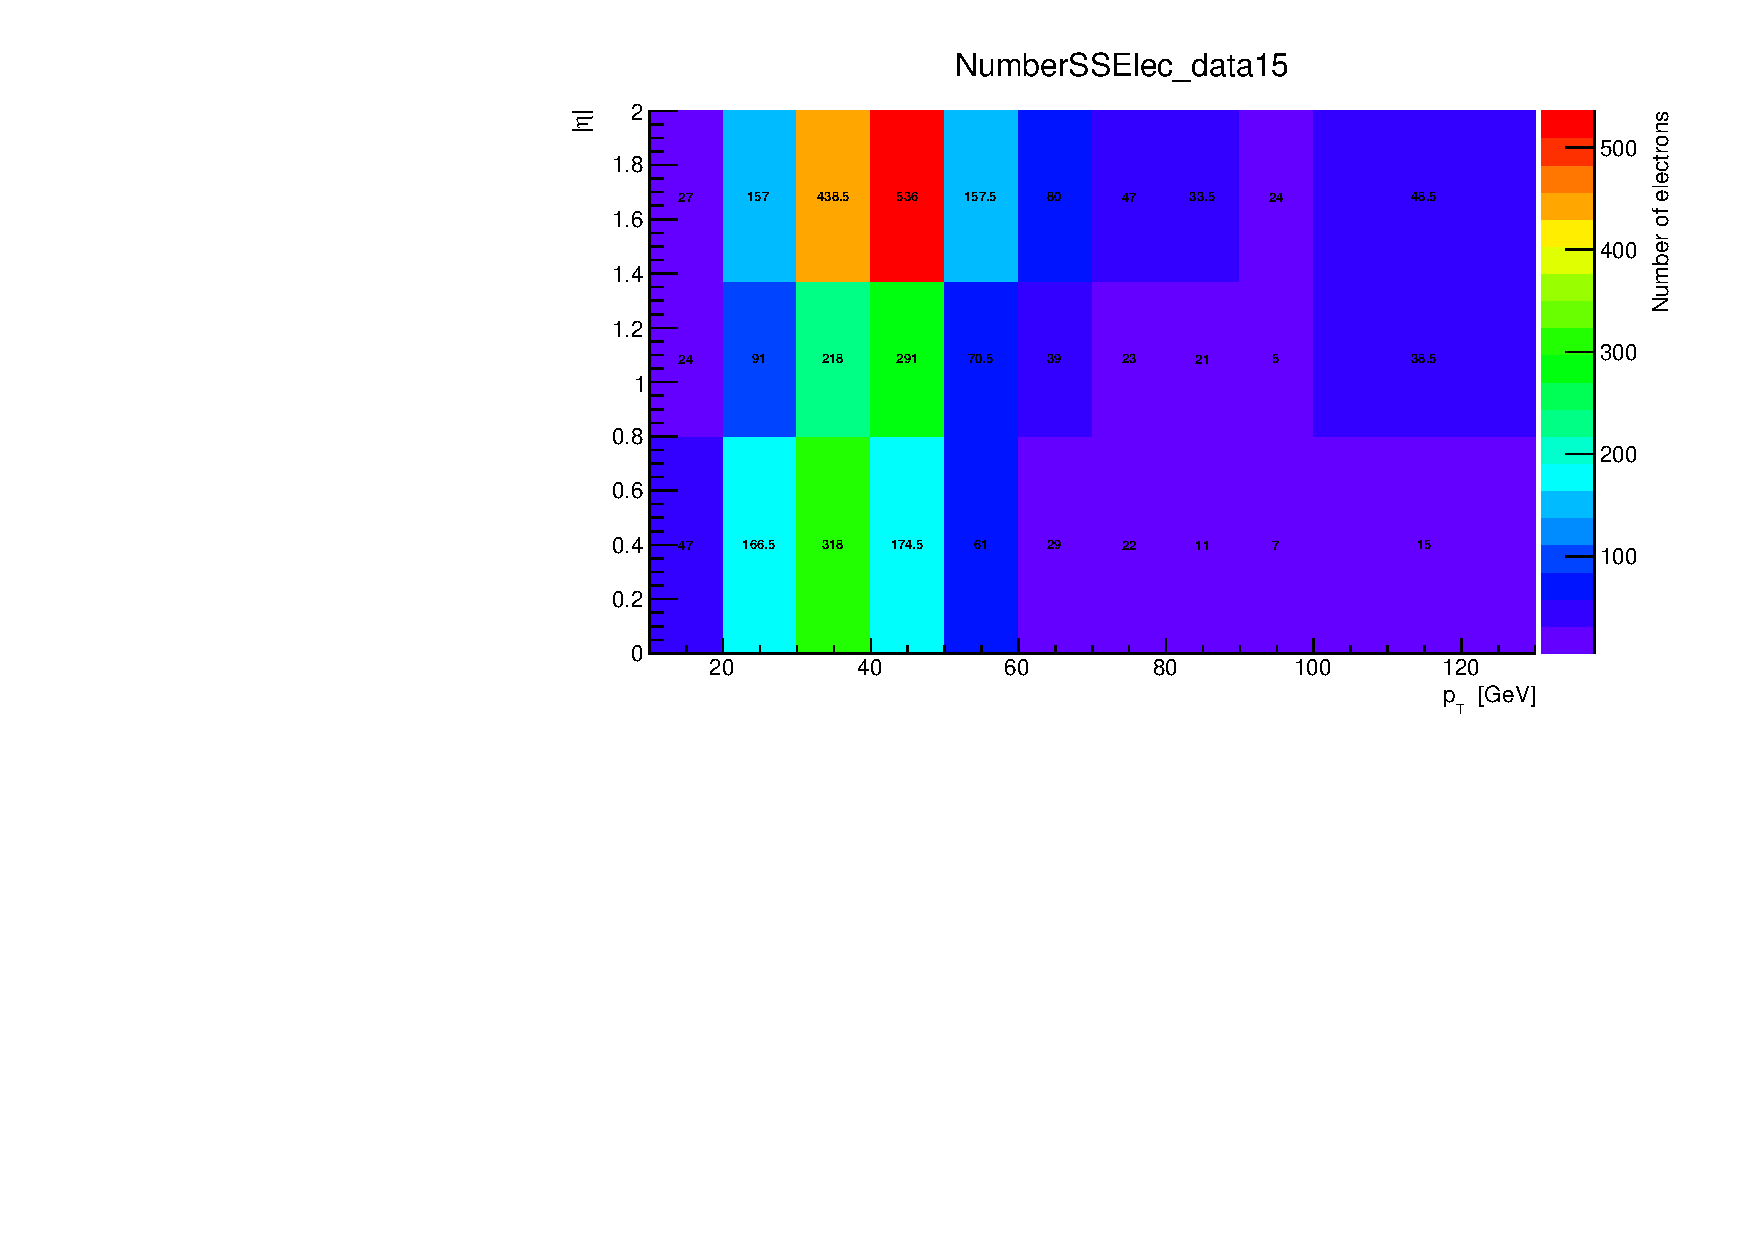
\includegraphics[width=0.65\textwidth]{FIGURES/BKG/chargeFlip/2D_histo_NumberSSElec_data15.pdf}
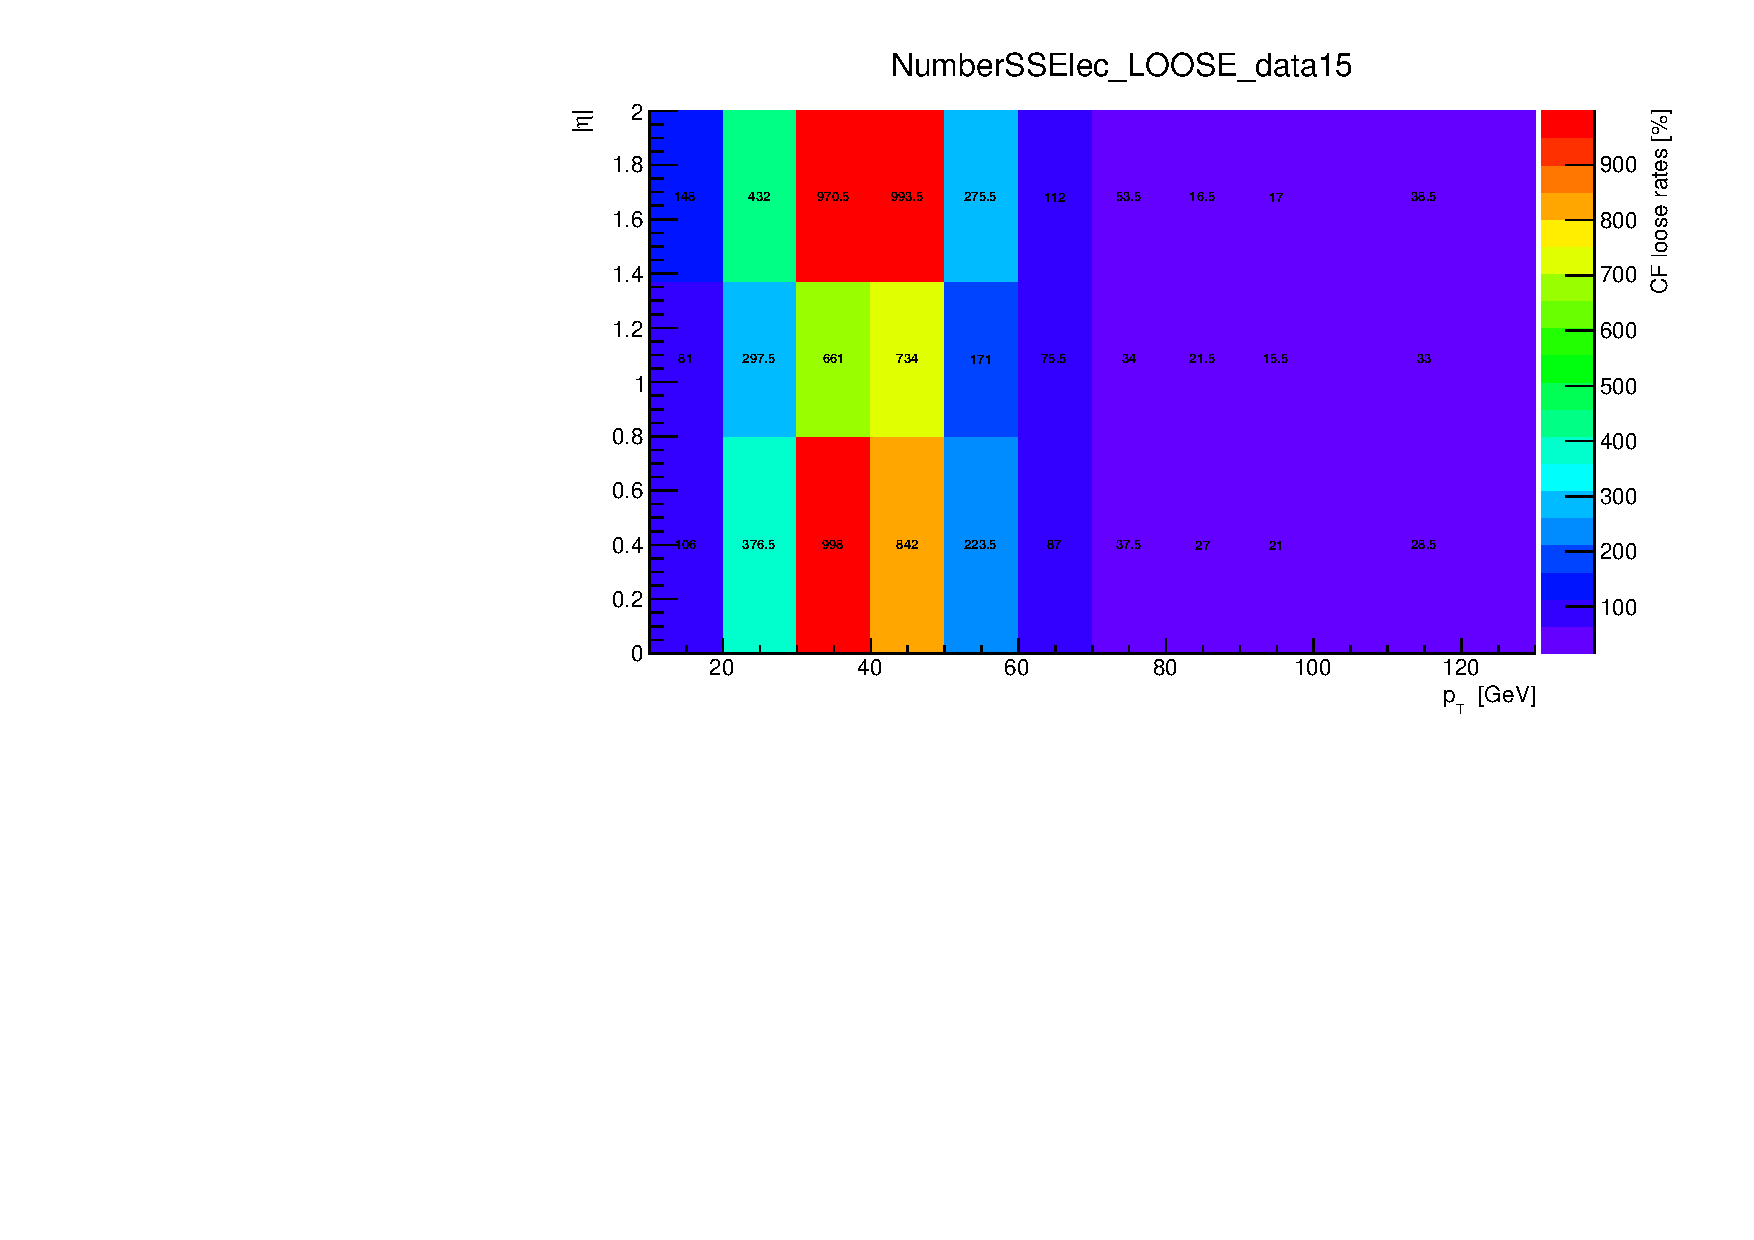
\includegraphics[width=0.65\textwidth]{FIGURES/BKG/chargeFlip/2D_histo_NumberSSElec_LOOSE_data15.pdf}
\caption{\label{fig:NSSdata} Number of electrons which form a same-sign event in 40 ($pt , | \eta | $) bins, used to compute the charge flip rates for the NOMINAL (top) and LOOSE (bottom) measurement  extracted from data, where the higher $\pt$ bins contain the overflow.}
\end{figure}
%------------------------------------------------

The nominal and loose rates extracted with data samples are presented respectively on Figure~\ref{fig:CFdata} extracted in data, where the higher $\pt$ bins contain the overflow. On Figure~\ref{fig:CFdata}, one can see that the expected trend, charge flip rate values are greater for higher $\pt$ and $\eta$ bins, is confirmed. On the top plot, the nominal measurement goes up to 0.75\% in the barrel region ($0.0<|\eta|<1.37$) while it goes up to 3.7\% in region $1.52<|\eta|<2.0$. On the bottom plot, the loose measurements are in general greater than the nominal ones in every bins and the rates goes up to 7.4\% in the barrel region ($0.0<|\eta|<1.37$) while it goes up to 10.8\% in region $1.52<|\eta|<2.0$. Another way to observe the charge flip dependancy on $\pt$ and $\eta$ is to plot all the rates on the same figures in function of $\pt$ as shown on Figure~\ref{fig:CFvsPt} where the $0.0<|\eta|<0.8$ range are shown in blue, the $0.8<|\eta|<1.37$ range in green and the $1.37<|\eta|<2.0$ range in orange. Despite some variations for the loose measurement in high $\pt$ bins, one can see that charge flip rates become greater when the $\pt$ value, as well as the $\eta$ value, increases.

%------------------------------------------------
\begin{figure}[!htb]
\centering
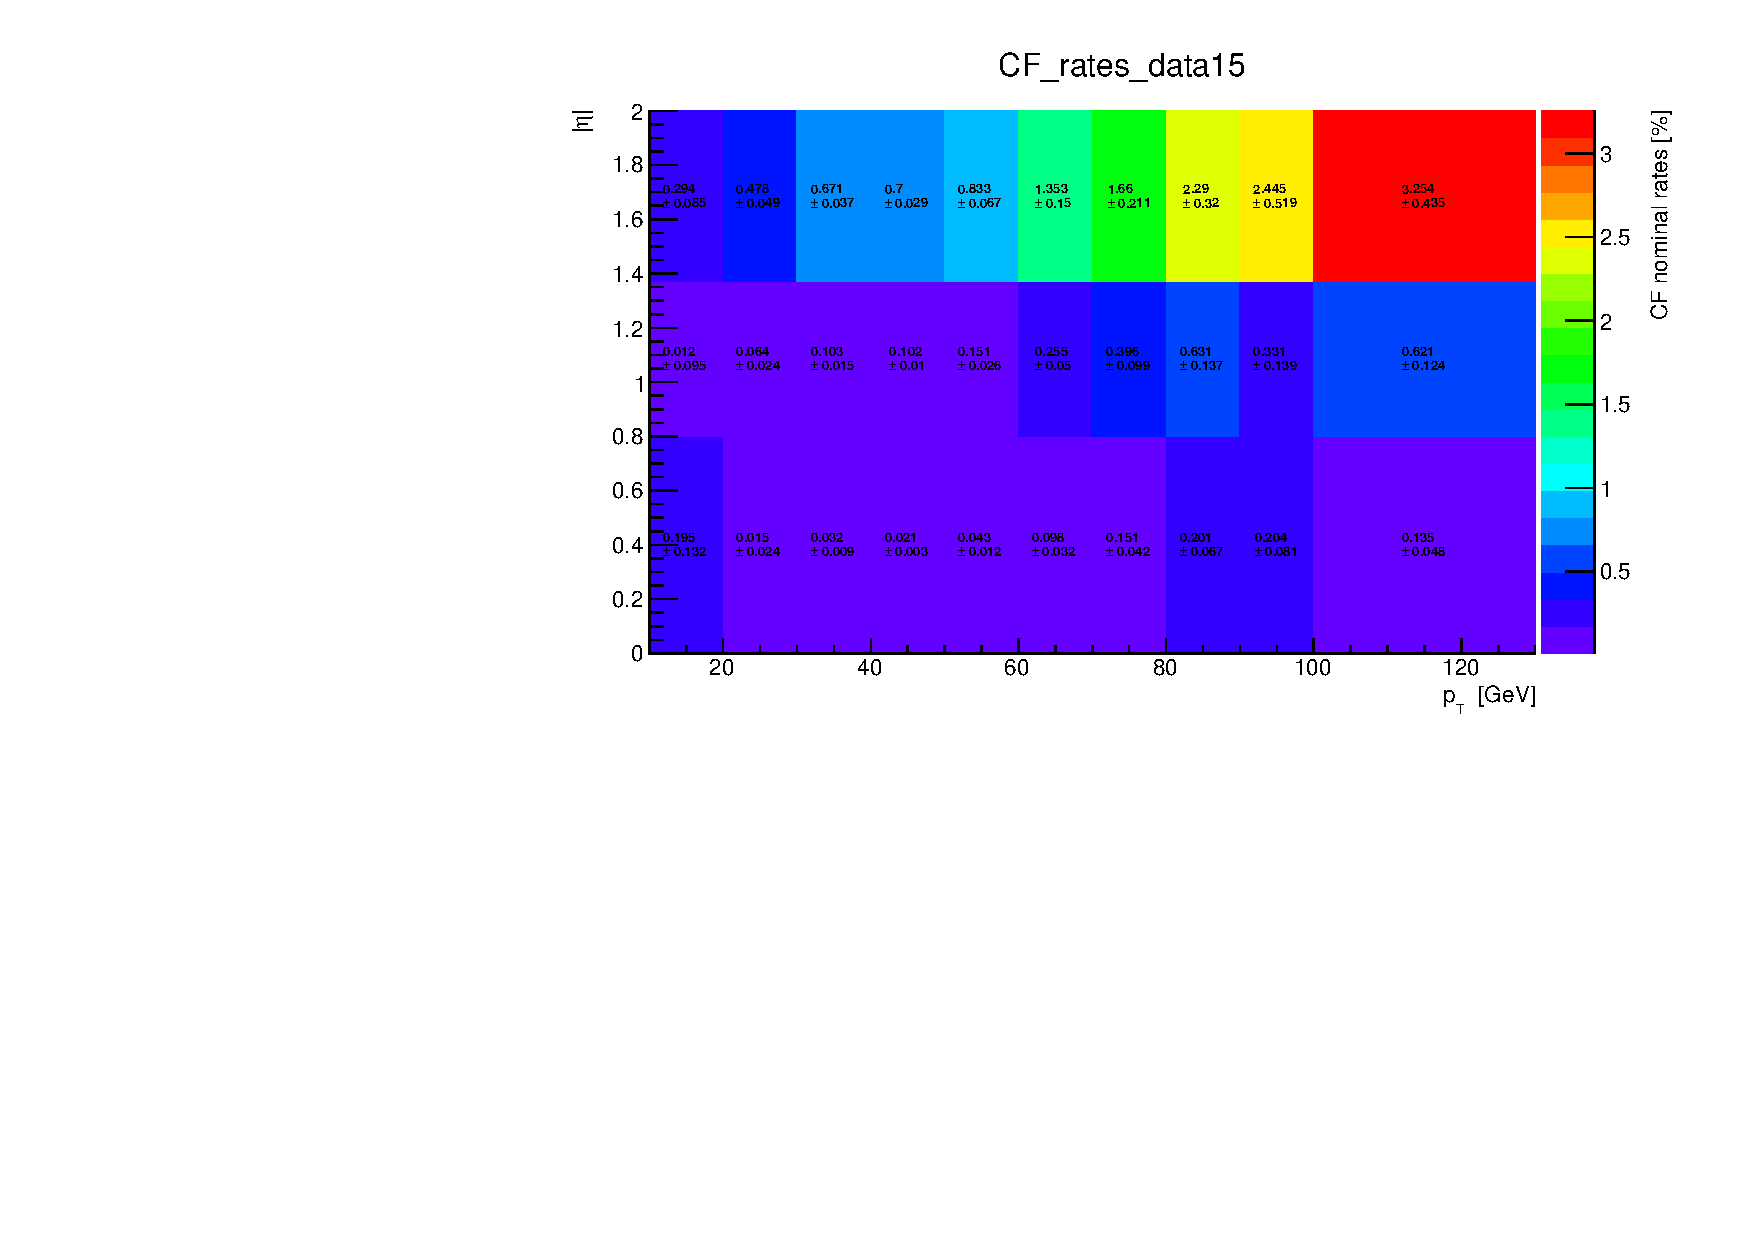
\includegraphics[width=0.65\textwidth]{FIGURES/BKG/chargeFlip/2D_histo_CF_rates_data15.pdf}

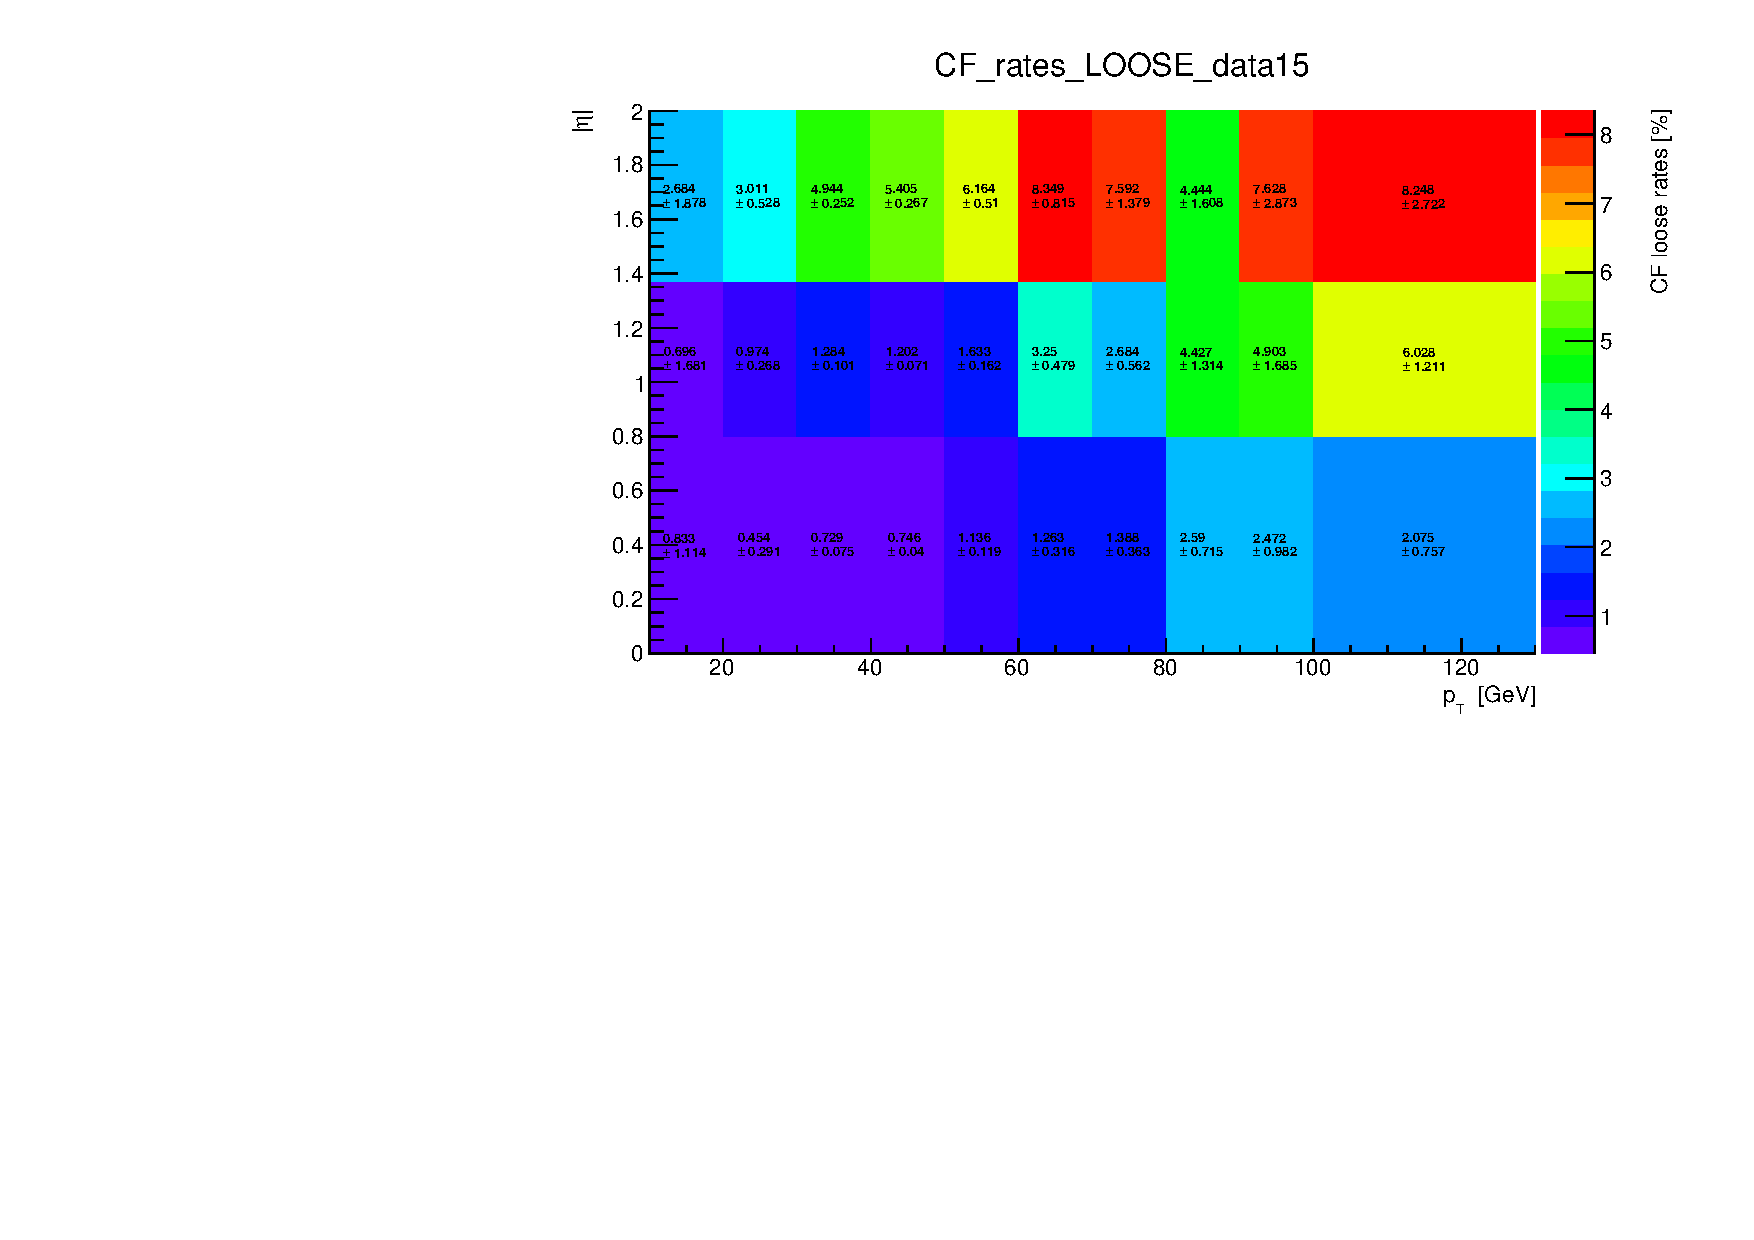
\includegraphics[width=0.65\textwidth]{FIGURES/BKG/chargeFlip/2D_histo_CF_rates_LOOSE_data15.pdf}
\caption{\label{fig:CFdata} Mis-identification rates in 40 ($pt , |\eta| $) bins with their respective statistical+systematic uncertainties for the NOMINAL (top) and LOOSE (bottom) measurement extracted in data, where the higher $\pt$ bins contain the overflow.}
\end{figure}
%------------------------------------------------

%------------------------------------------------
\begin{figure}[!htb]
\centering
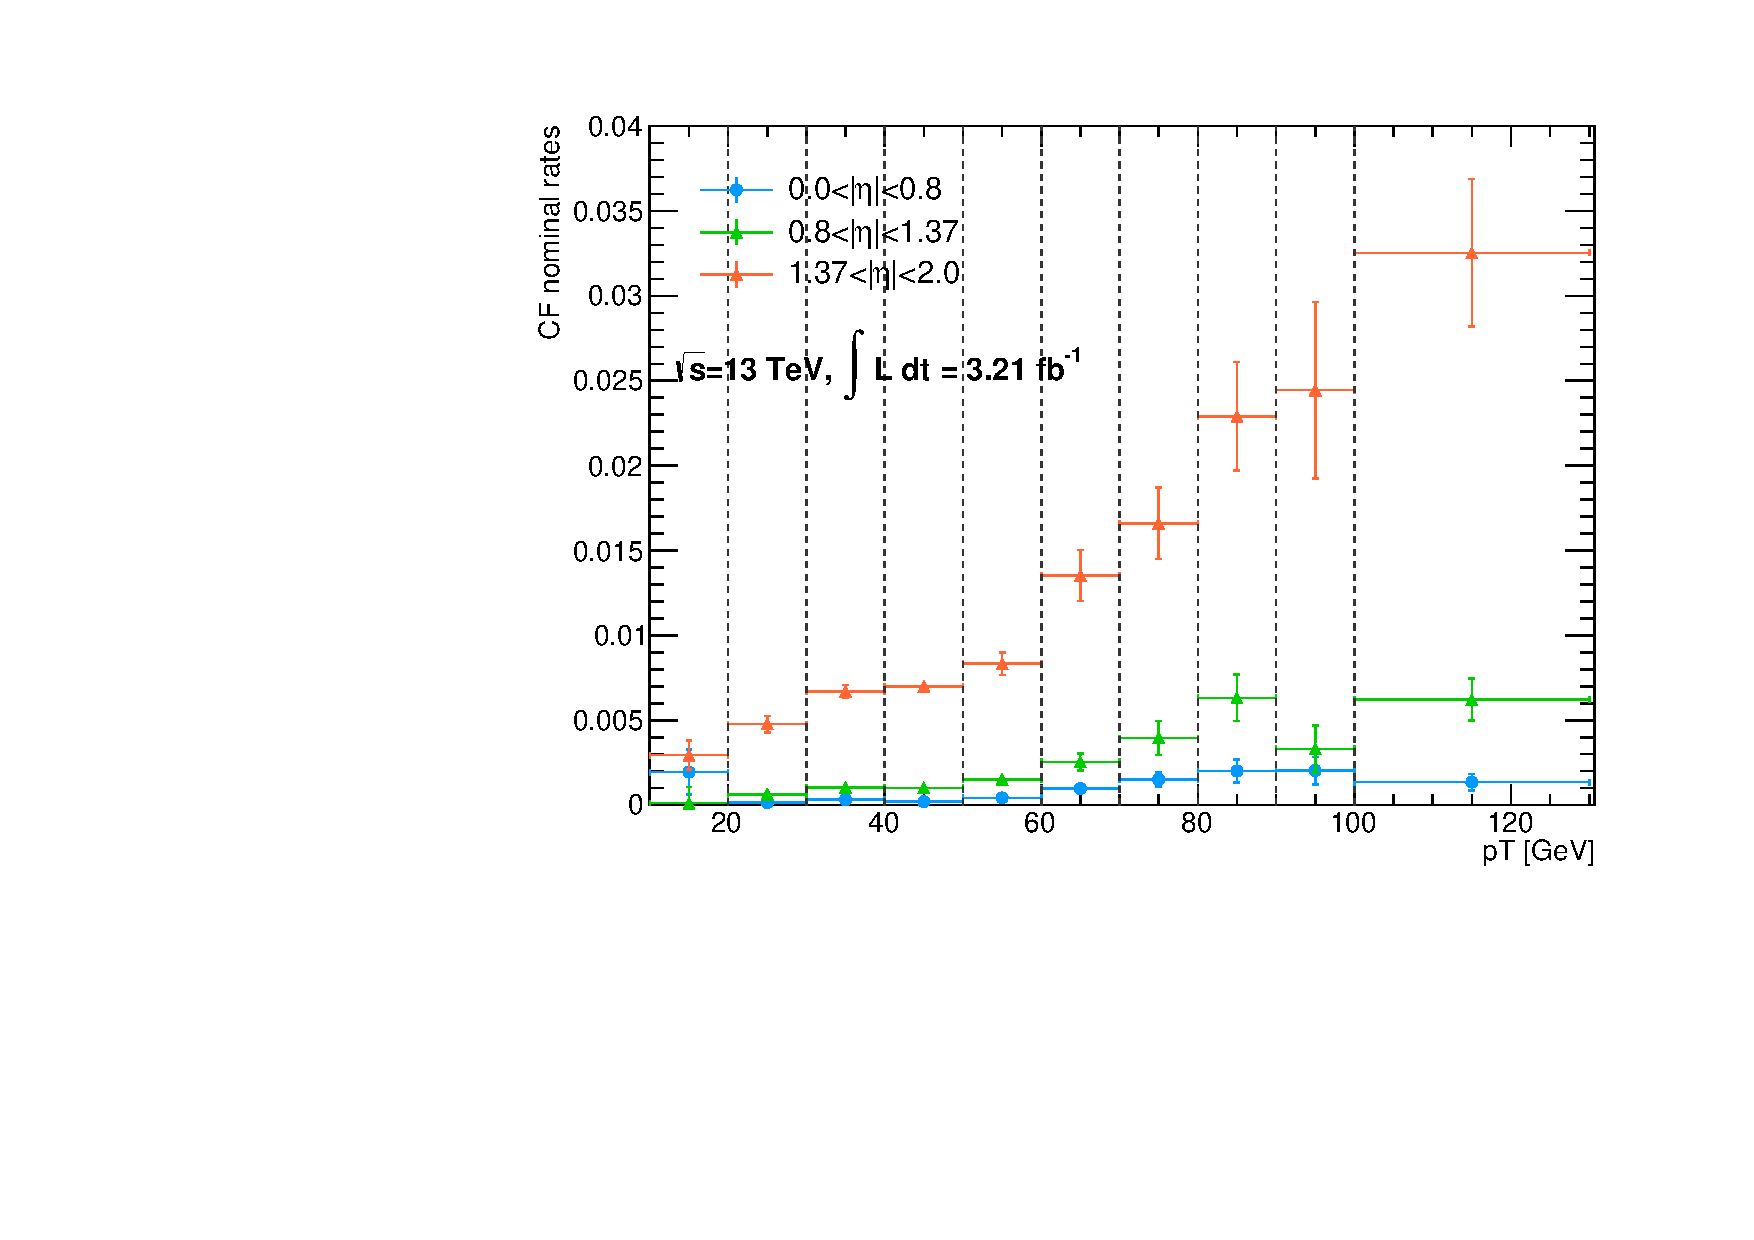
\includegraphics[width=0.65\textwidth]{FIGURES/BKG/chargeFlip/CFratesVSpt_data15.pdf}

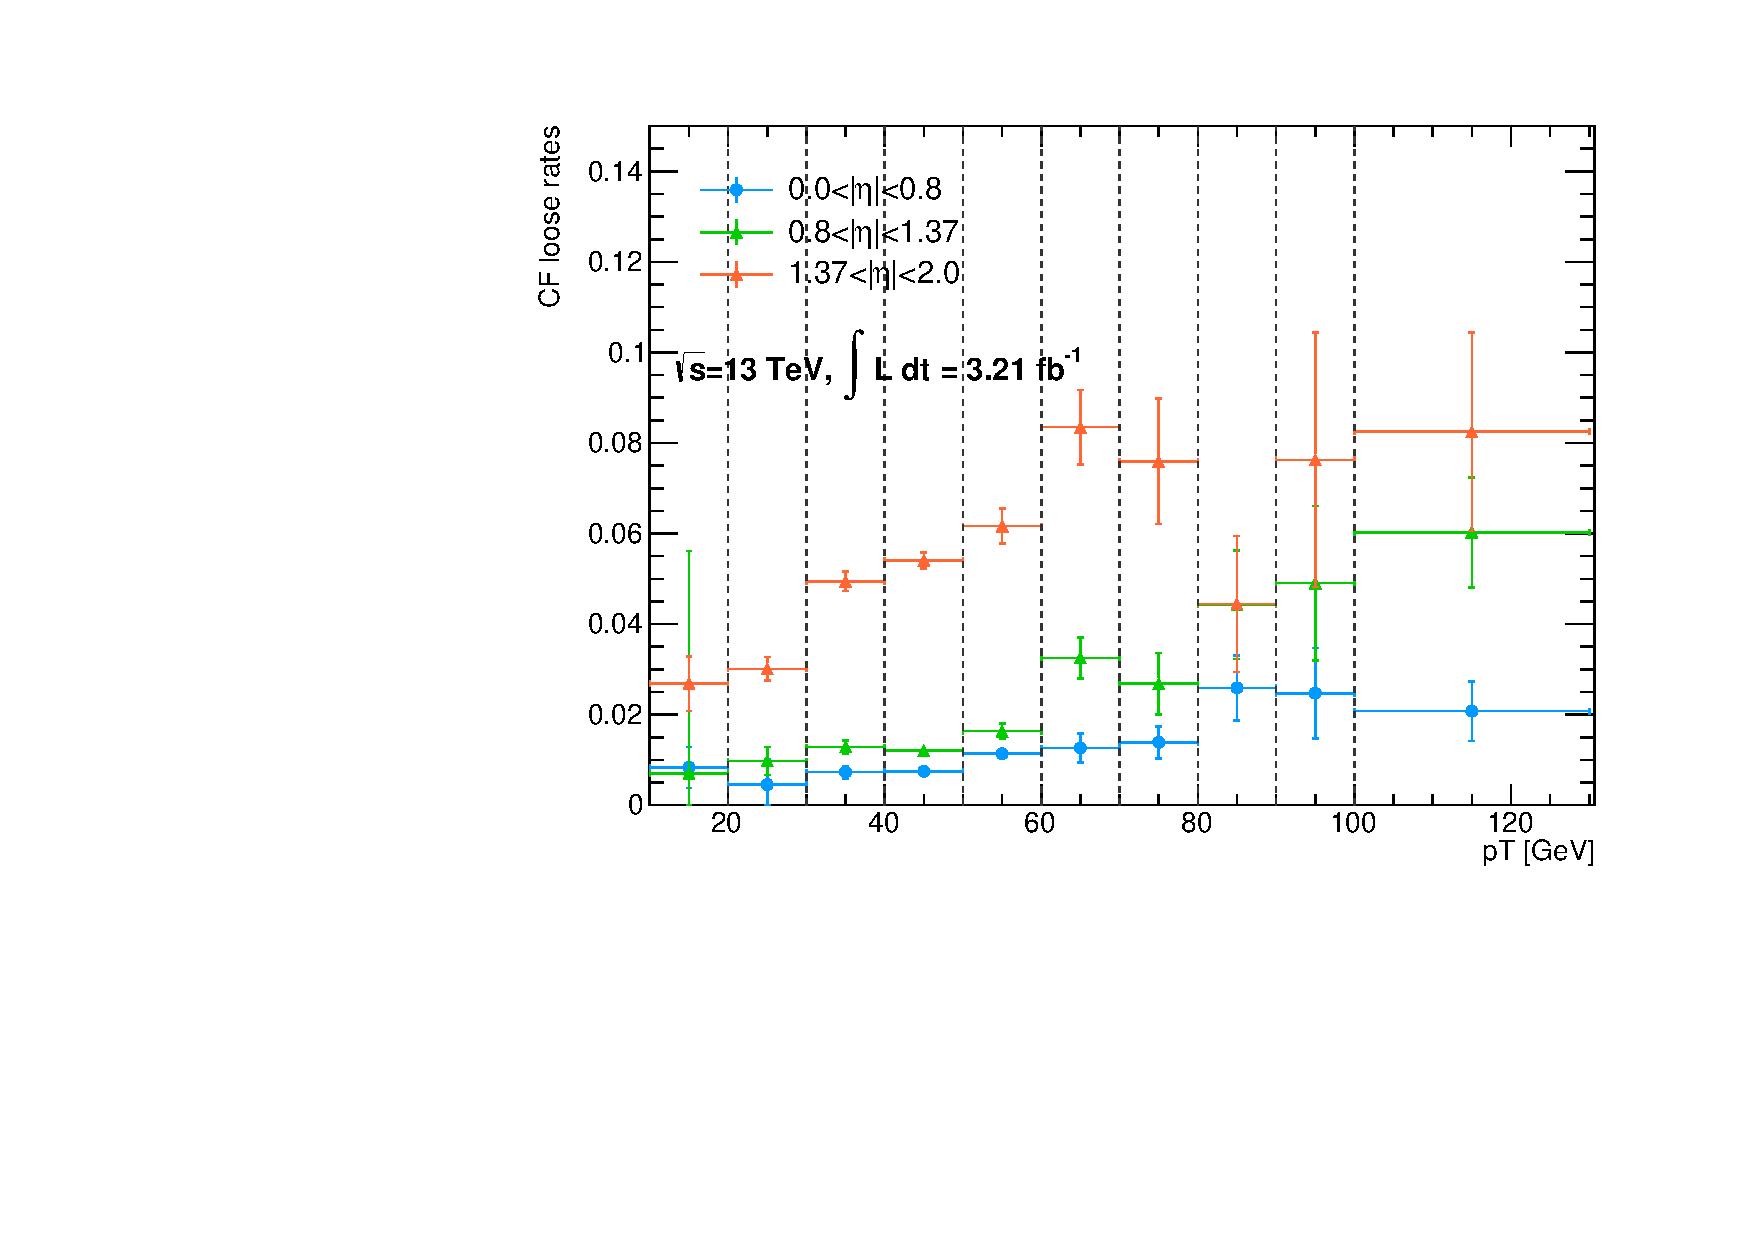
\includegraphics[width=0.65\textwidth]{FIGURES/BKG/chargeFlip/CFratesVSpt_LOOSE_data15.pdf}
\caption{\label{fig:CFvsPt} Mis-identification rates in function of the $\pt$ distribution for three different $\eta$ ranges: $0.0<|\eta|<0.8$ in blue, $0.8<|\eta|<1.37$ in green and $1.37<|\eta|<2.0$ in orange. Statistical and systematic uncertainties are include. The top (bottom) plot show nominal (loose) measurement extracted in data, where the higher $\pt$ bin contains the overflow.}
\end{figure}
%------------------------------------------------


The comparison of charge flip rates from data and from MC for nominal measurement is plotted for different $\pt$ range on Figure~\ref{fig:CFratesNominal_1}. The same comparison was done for the loose measurement, it is shown on Figure~\ref{fig:CFratesLoose_2} and are notably used in section~\ref{sec:bkg_VP_DD_estimates}. Again, one can see that the charge flip rates for the loose measurement are much larger than for the nominal measurement (typically by a factor 10), illustrating the necessity of this auxiliary measurement. From those plots, one can see a fairly good agreement between data and MC results. In low $\pt$ bins (below 40 GeV) in the nominal measurement, MC predictions seem to overestimate the charge flip rates at high $|\eta|$ ($1.52<|\eta|<2.0$). For the loose measurement, the same pattern appear in high $\pt$ region (above 60 GeV) in the last $|\eta|$ bin where one can see that MC predictions overestimate the charge flip rates obtained from data sample. Apart those small differences, the agreement between data and MC is good in general.

%------------------------------------------------
\begin{figure}[h!]
\centering
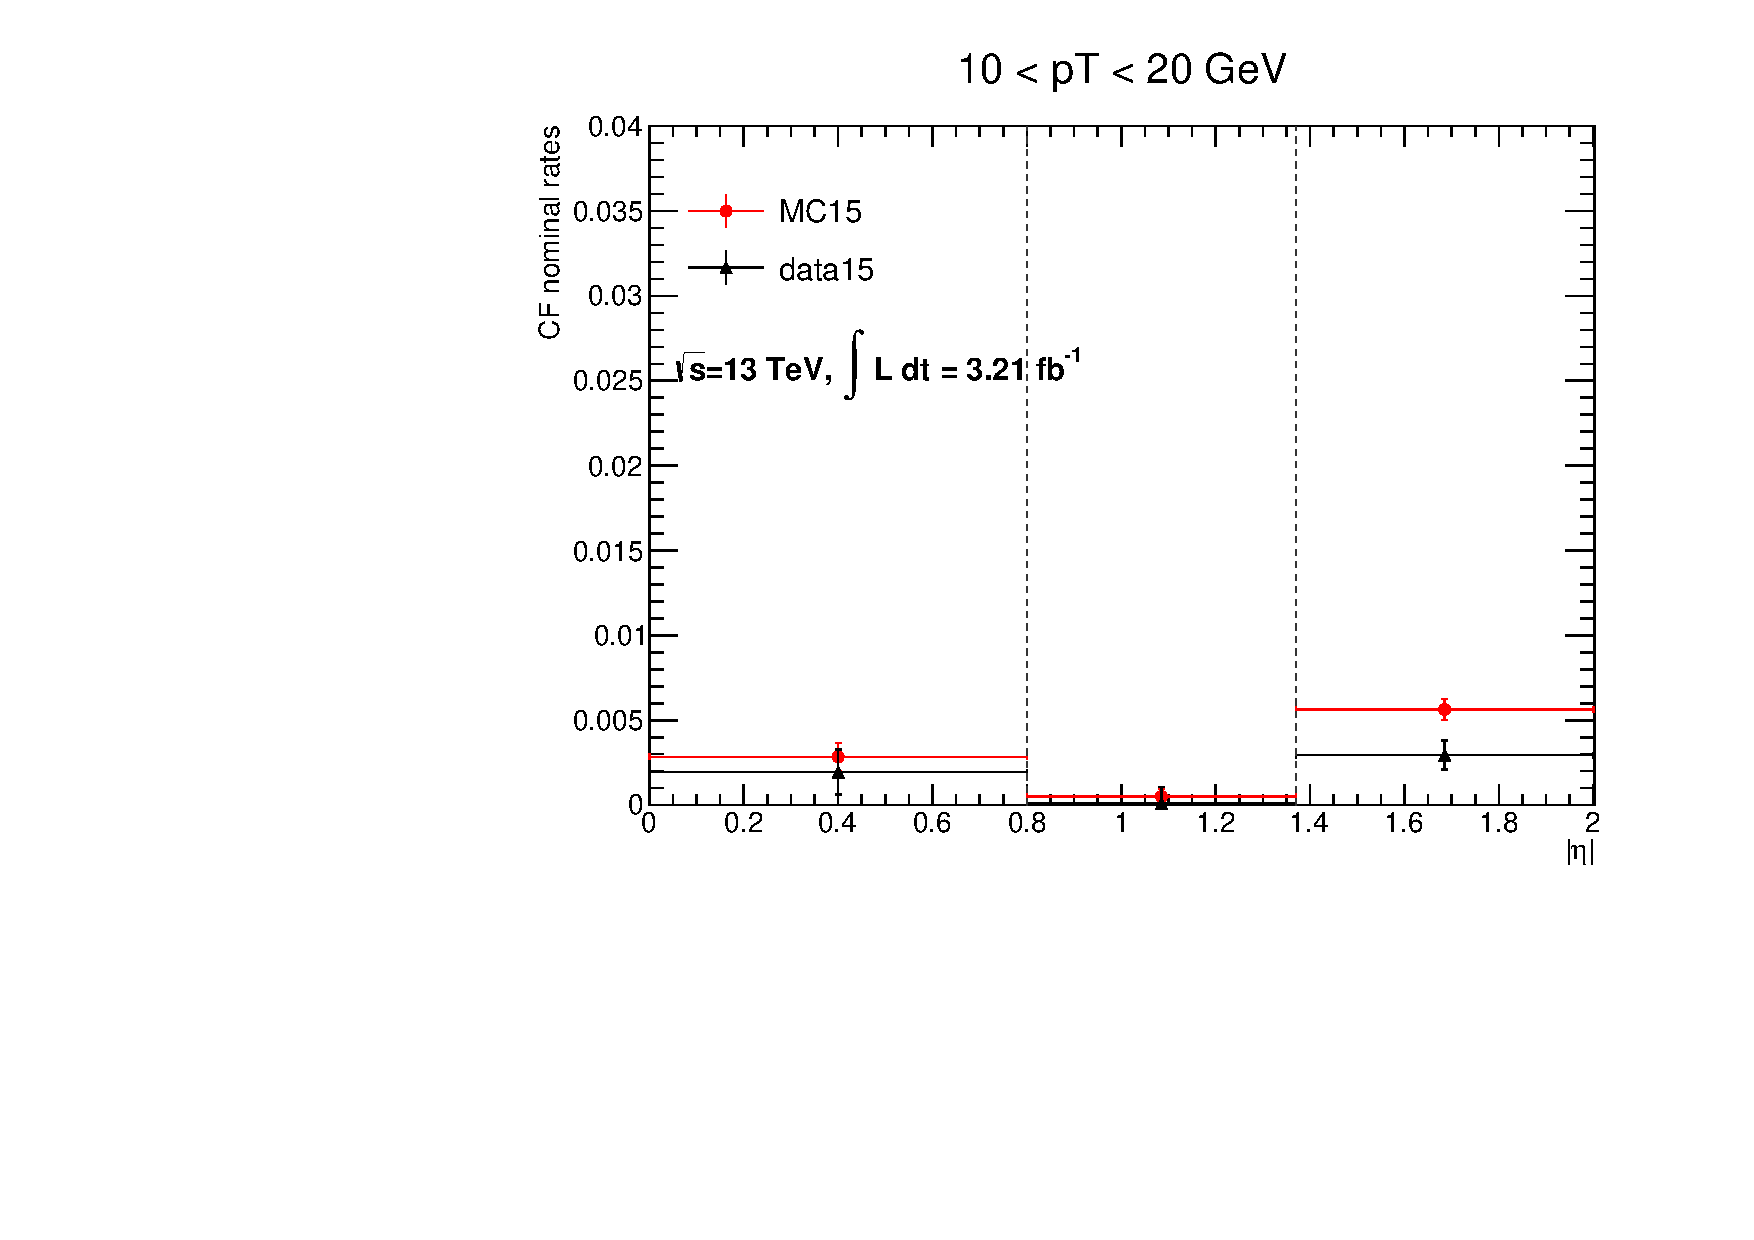
\includegraphics[width=0.4\textwidth]{FIGURES/BKG/chargeFlip/CFrates___dataVSmc___PTbin0.pdf}
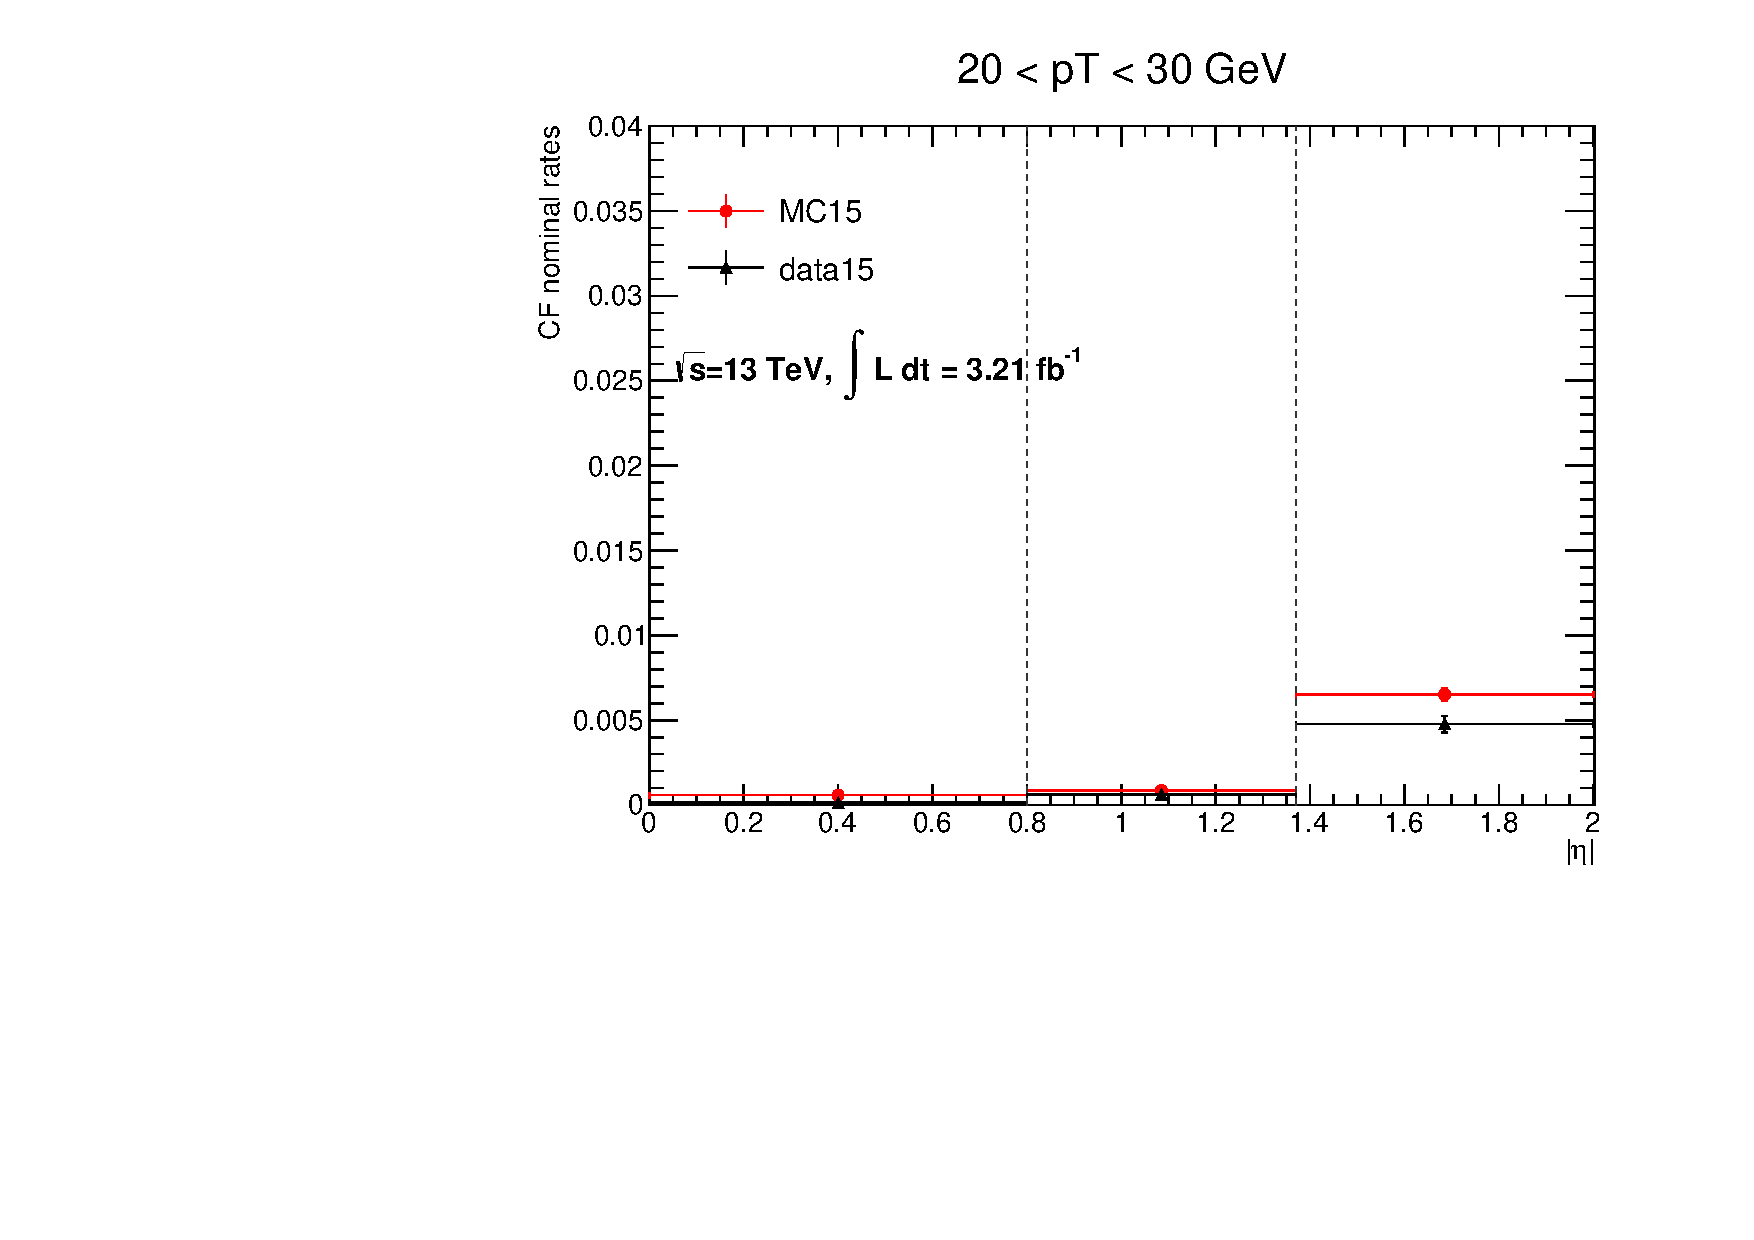
\includegraphics[width=0.4\textwidth]{FIGURES/BKG/chargeFlip/CFrates___dataVSmc___PTbin1.pdf}
\vfill
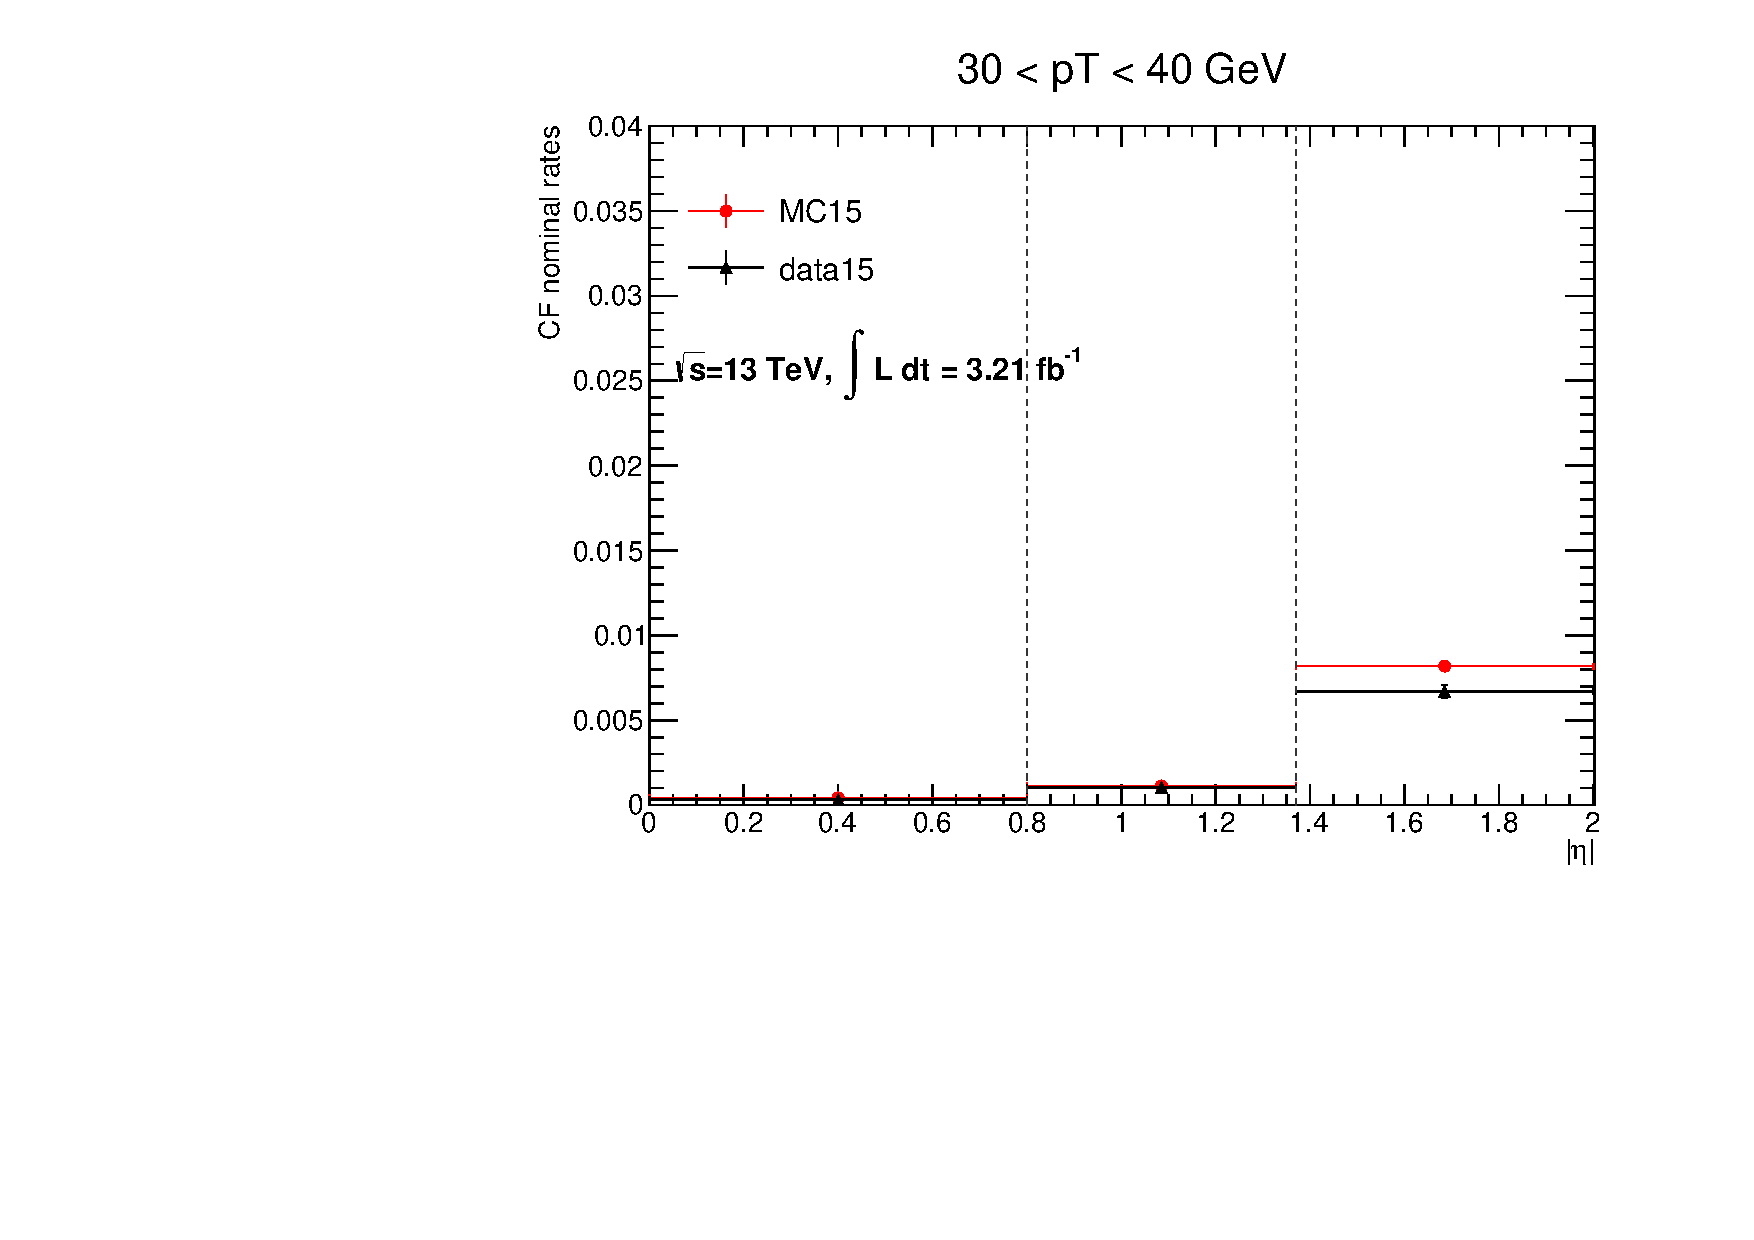
\includegraphics[width=0.4\textwidth]{FIGURES/BKG/chargeFlip/CFrates___dataVSmc___PTbin2.pdf}
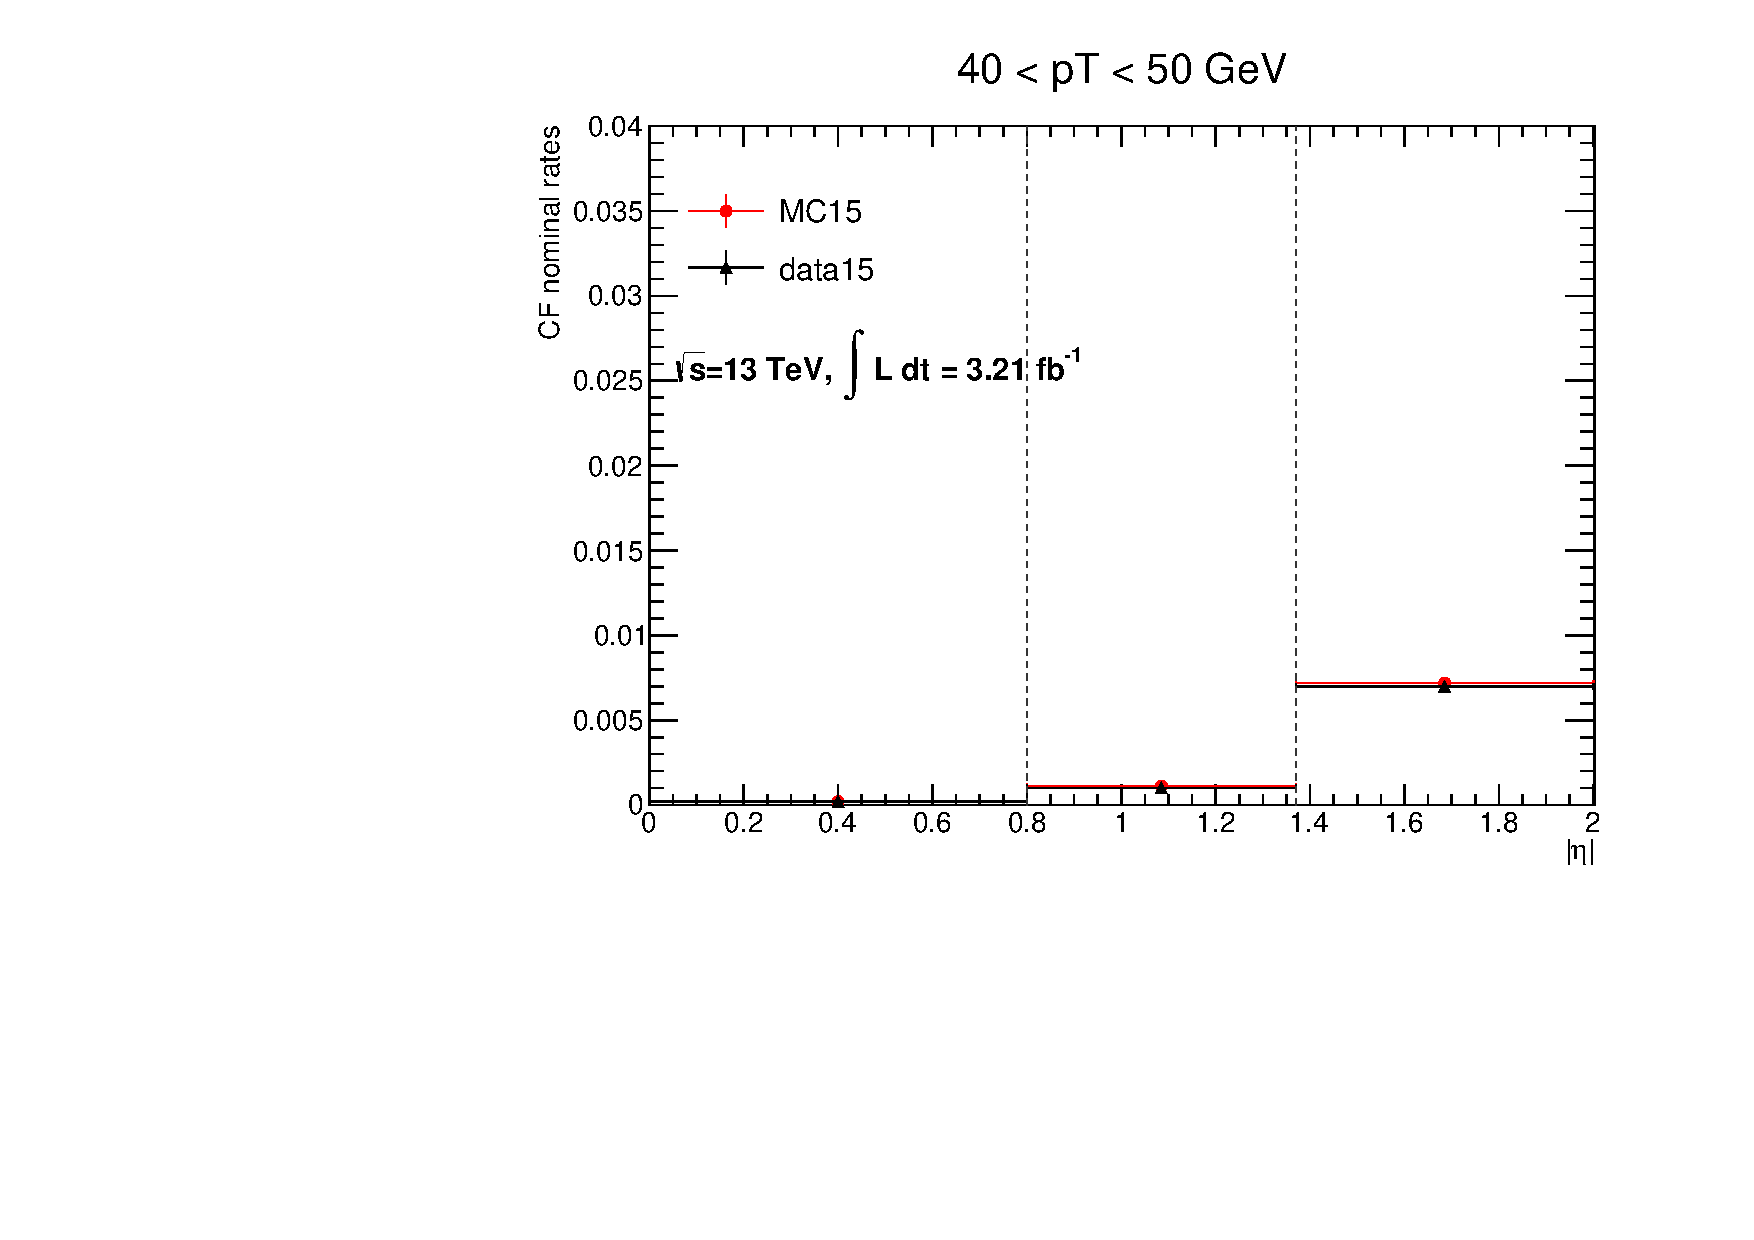
\includegraphics[width=0.4\textwidth]{FIGURES/BKG/chargeFlip/CFrates___dataVSmc___PTbin3.pdf}

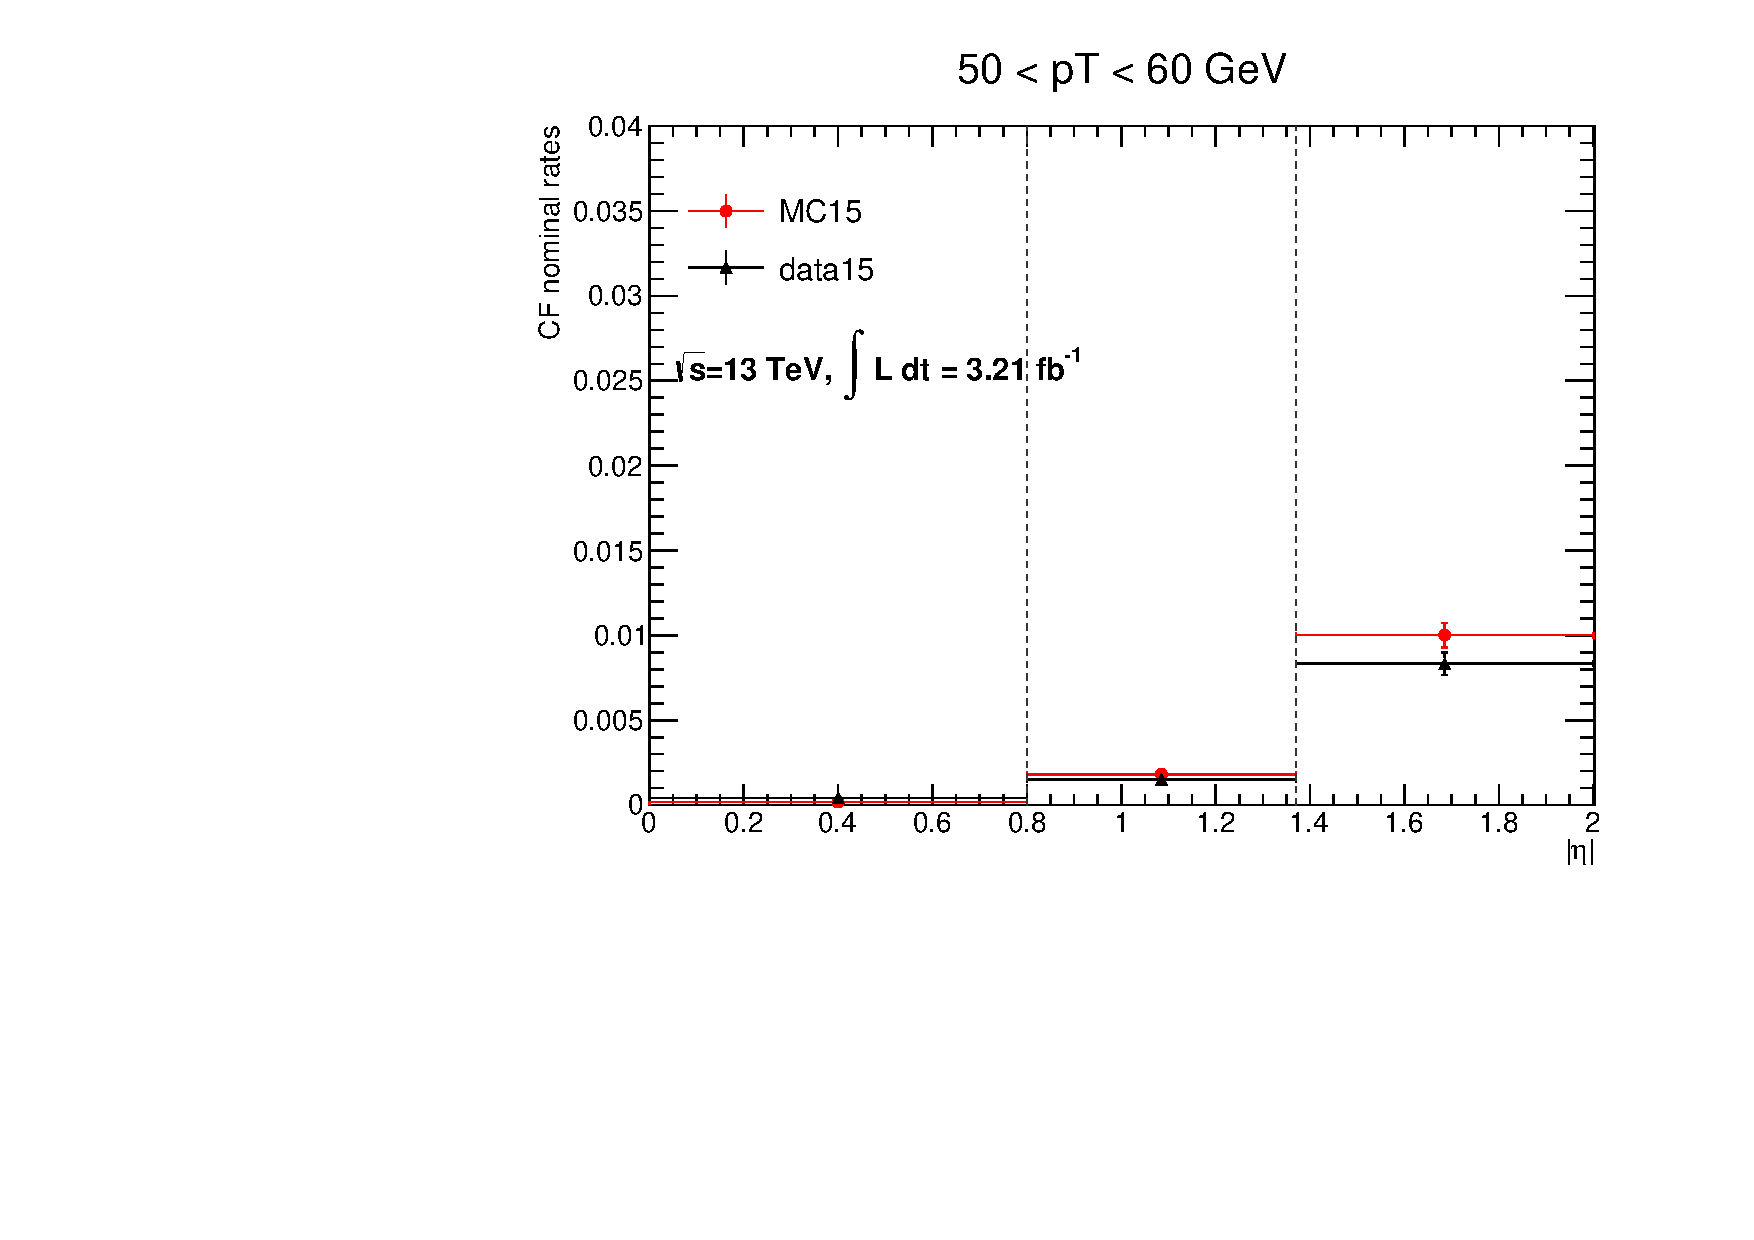
\includegraphics[width=0.4\textwidth]{FIGURES/BKG/chargeFlip/CFrates___dataVSmc___PTbin4.pdf}
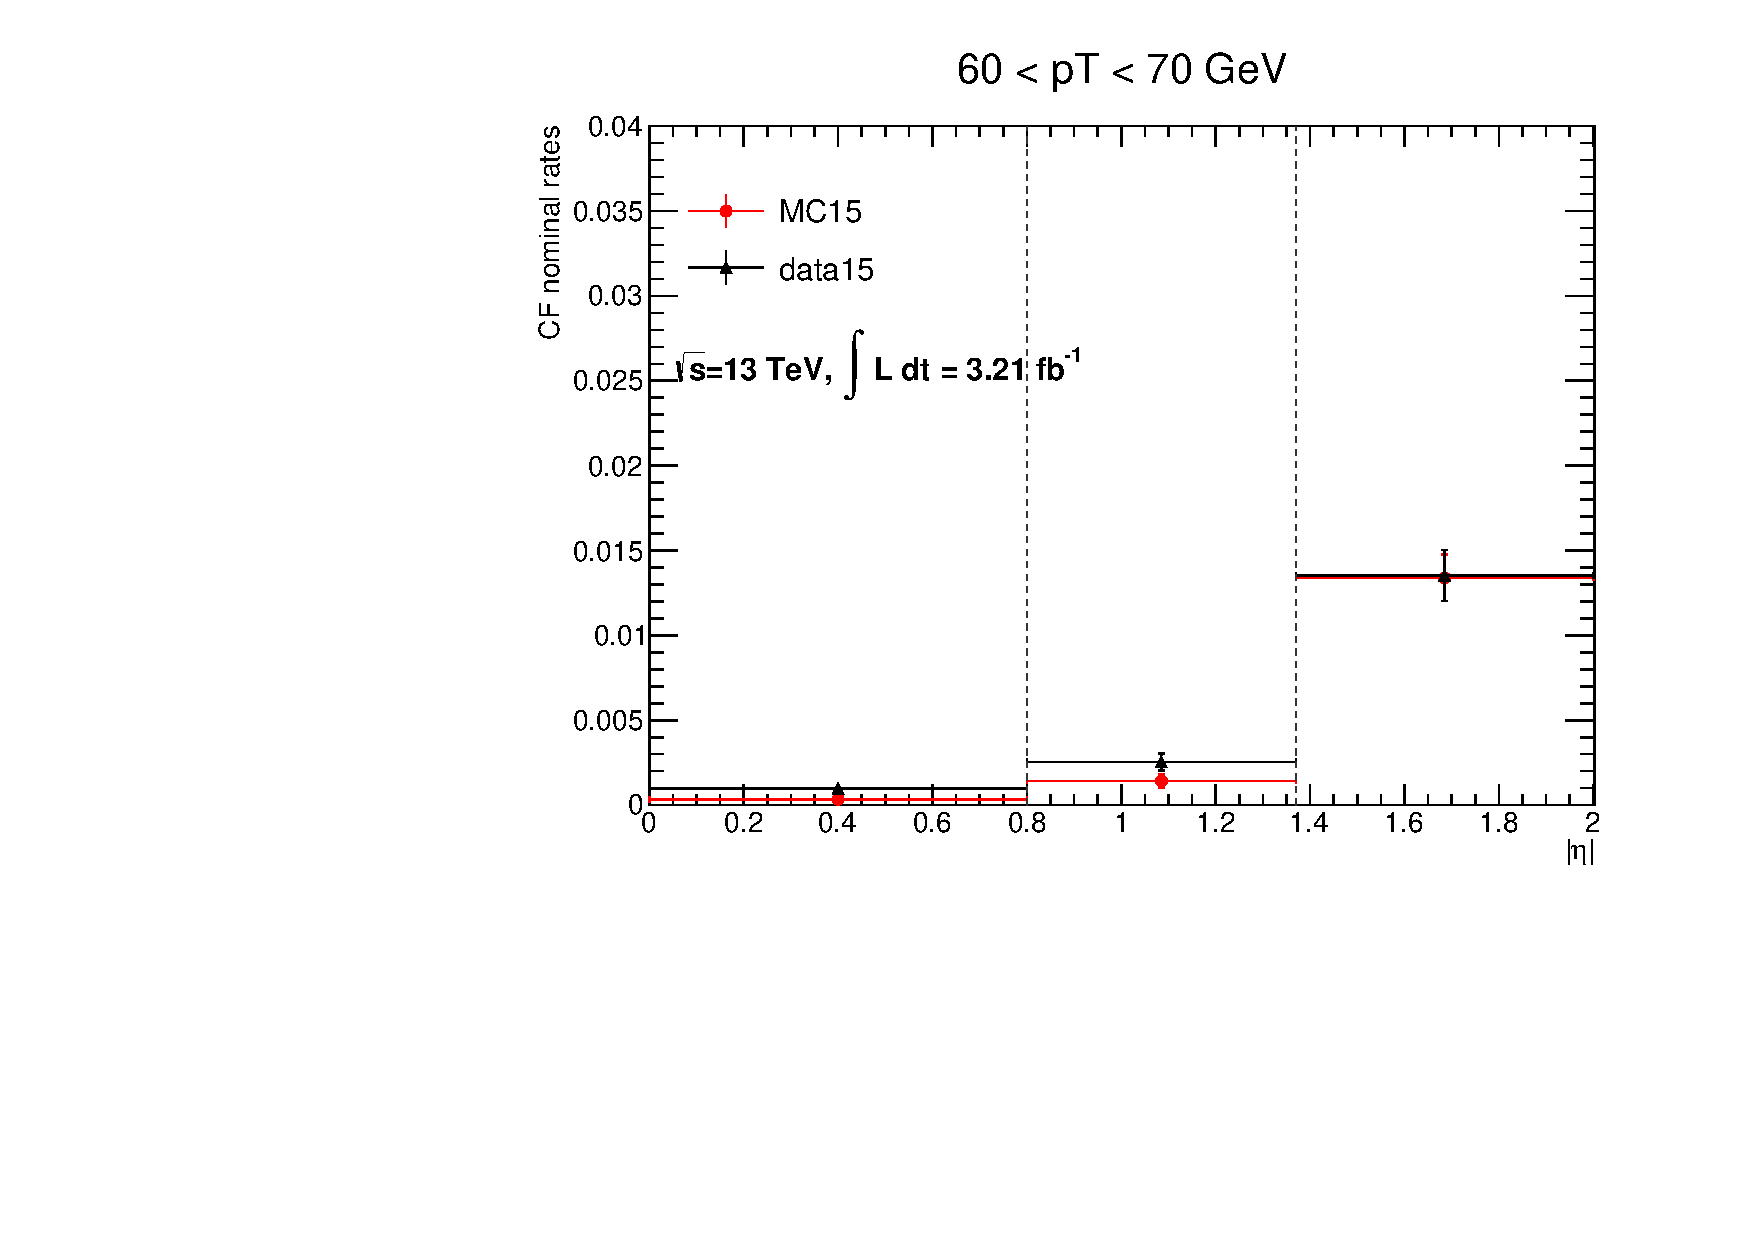
\includegraphics[width=0.4\textwidth]{FIGURES/BKG/chargeFlip/CFrates___dataVSmc___PTbin5.pdf}
\vfill
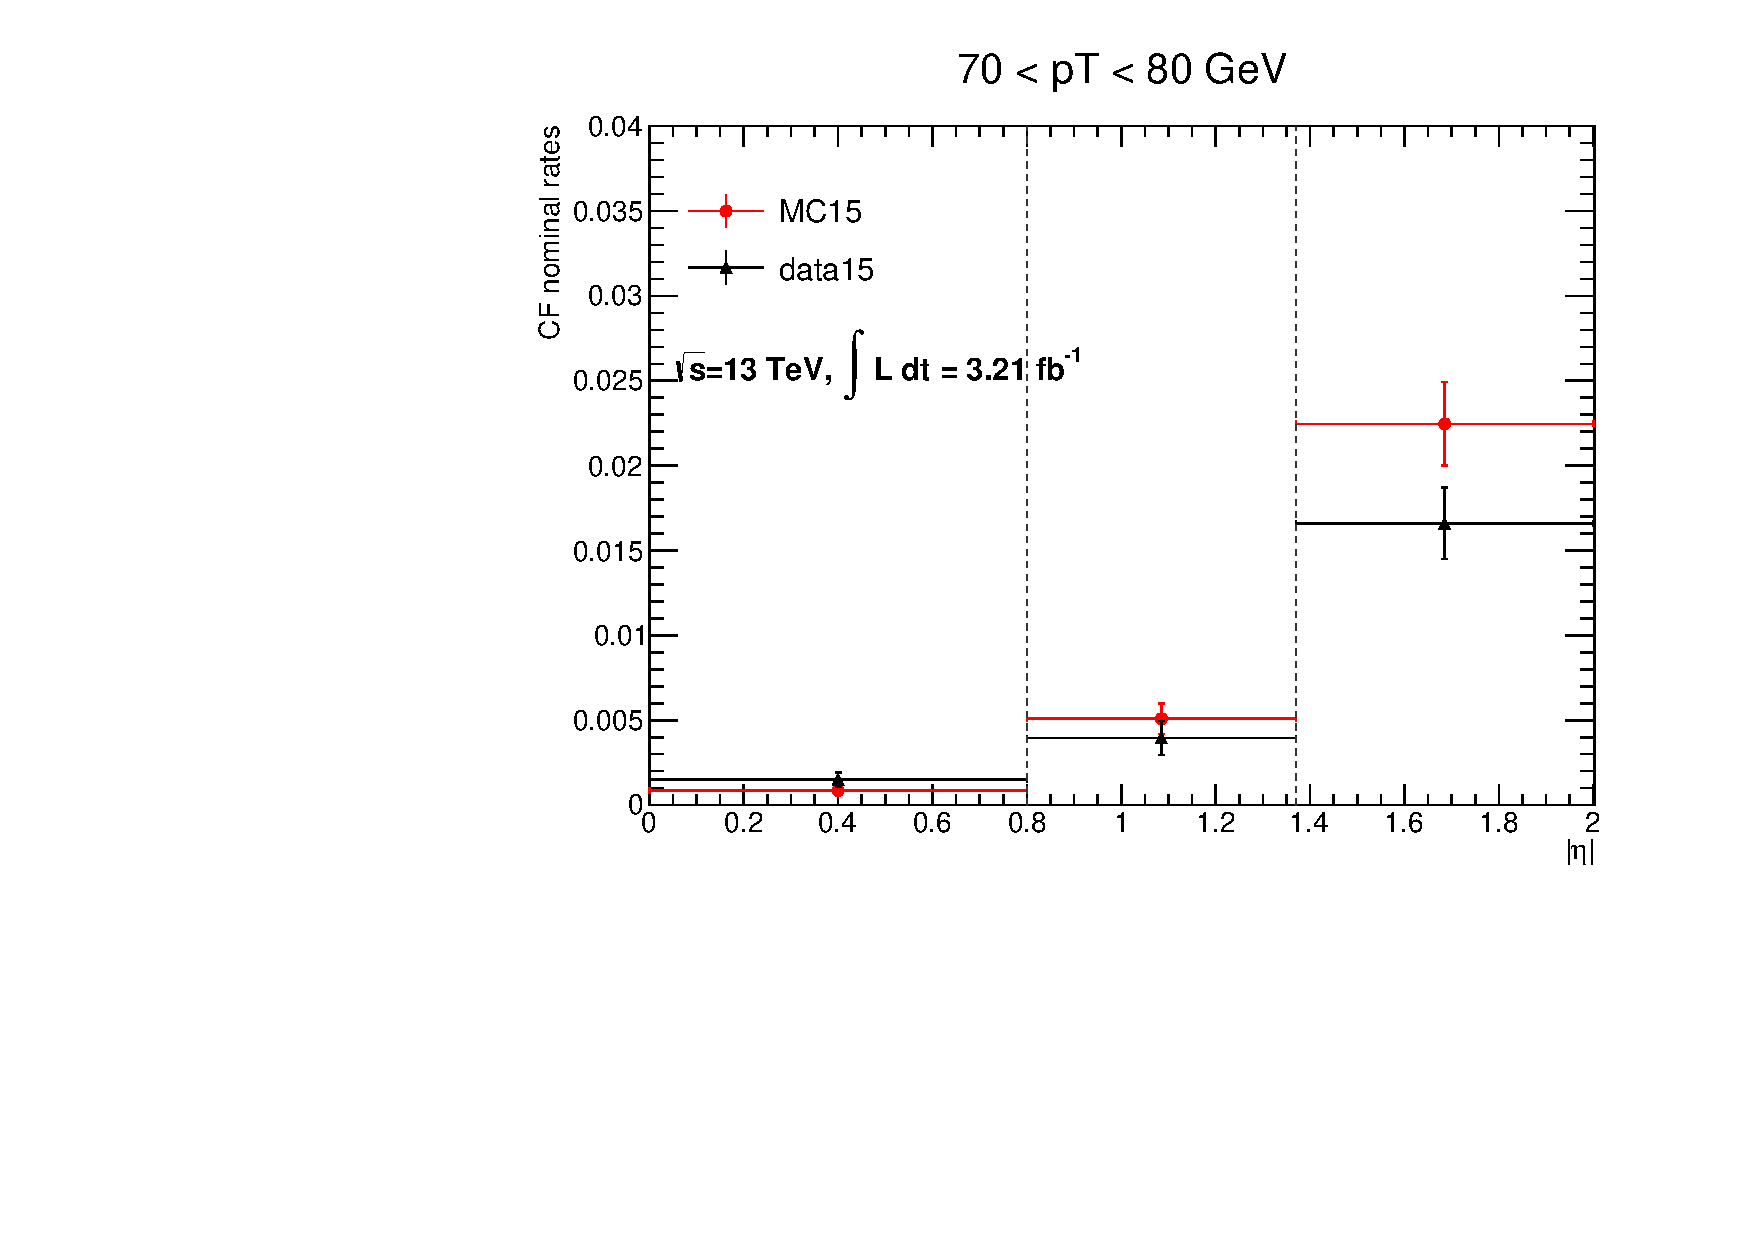
\includegraphics[width=0.4\textwidth]{FIGURES/BKG/chargeFlip/CFrates___dataVSmc___PTbin6.pdf}
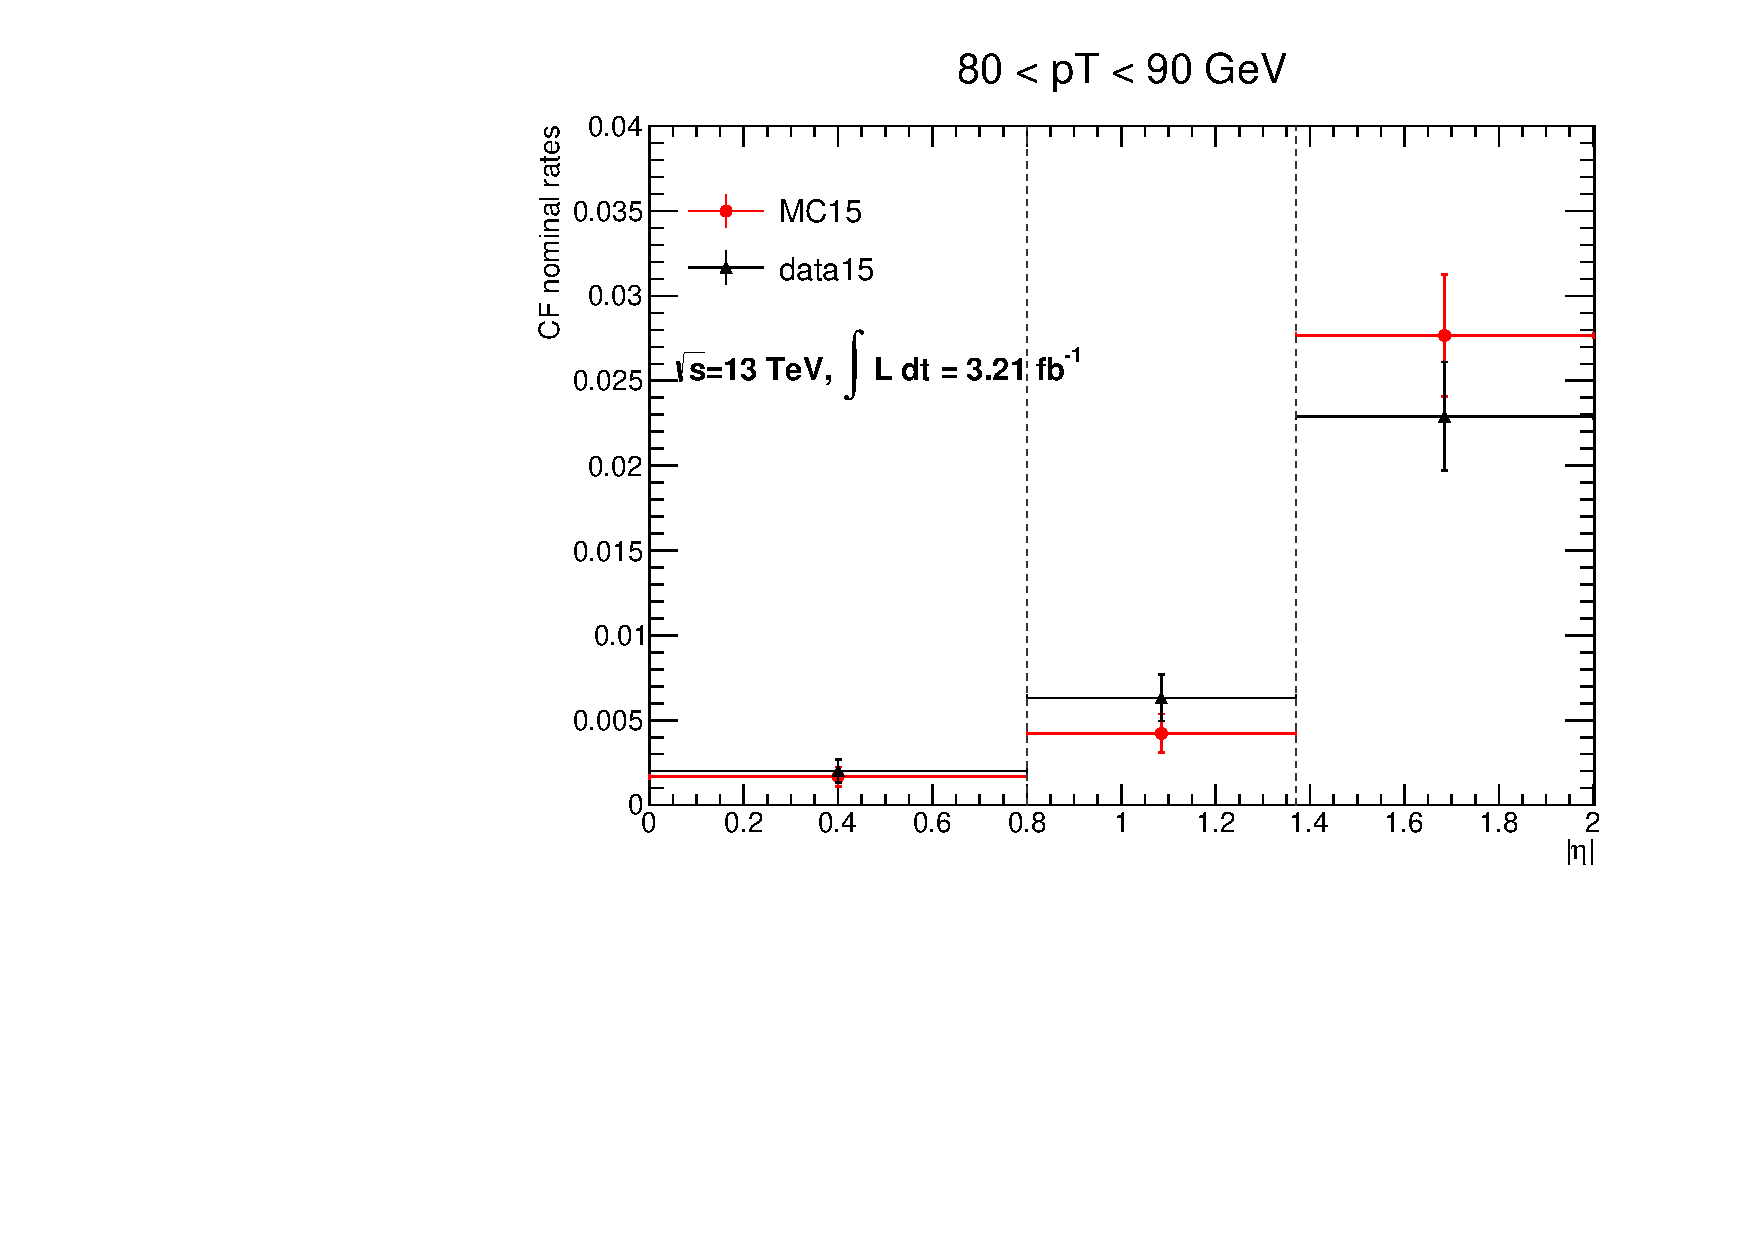
\includegraphics[width=0.4\textwidth]{FIGURES/BKG/chargeFlip/CFrates___dataVSmc___PTbin7.pdf}
\vfill
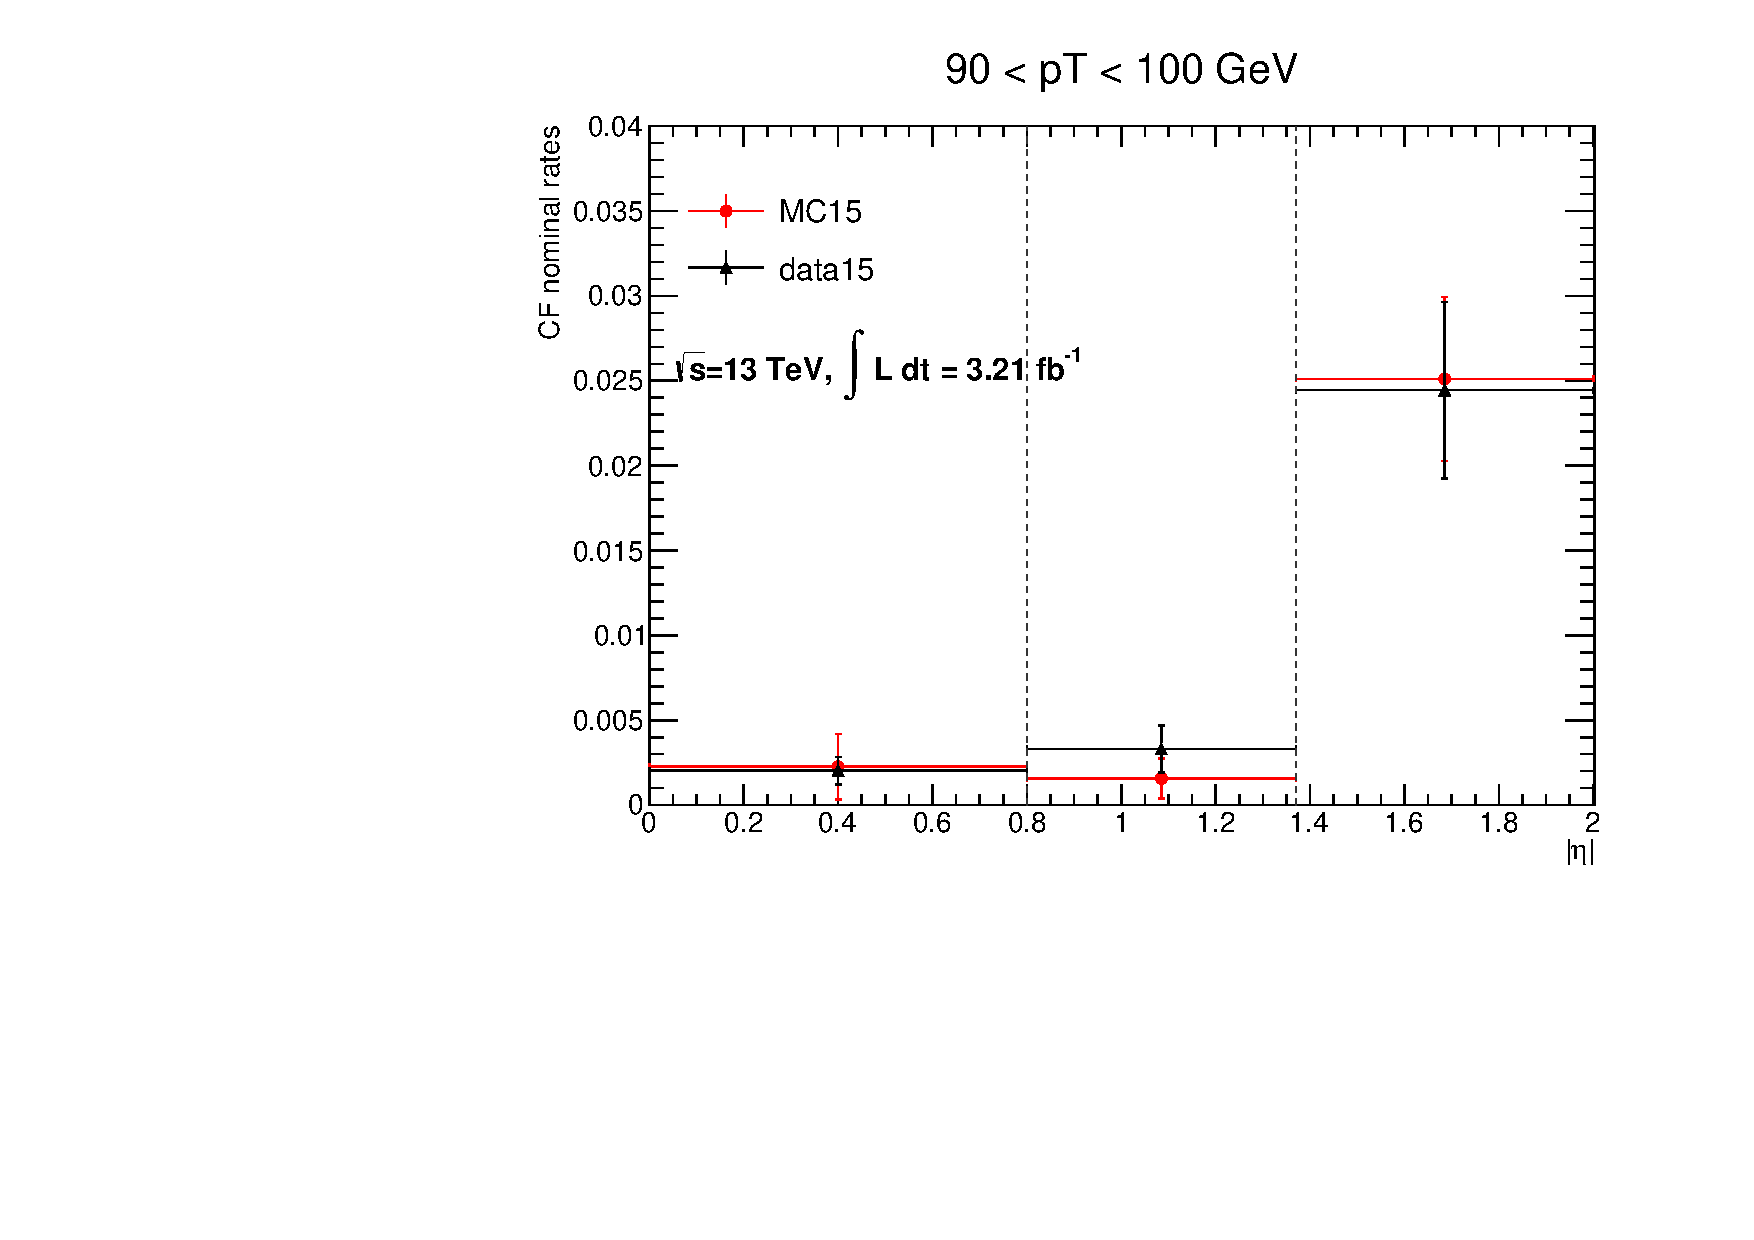
\includegraphics[width=0.4\textwidth]{FIGURES/BKG/chargeFlip/CFrates___dataVSmc___PTbin8.pdf}
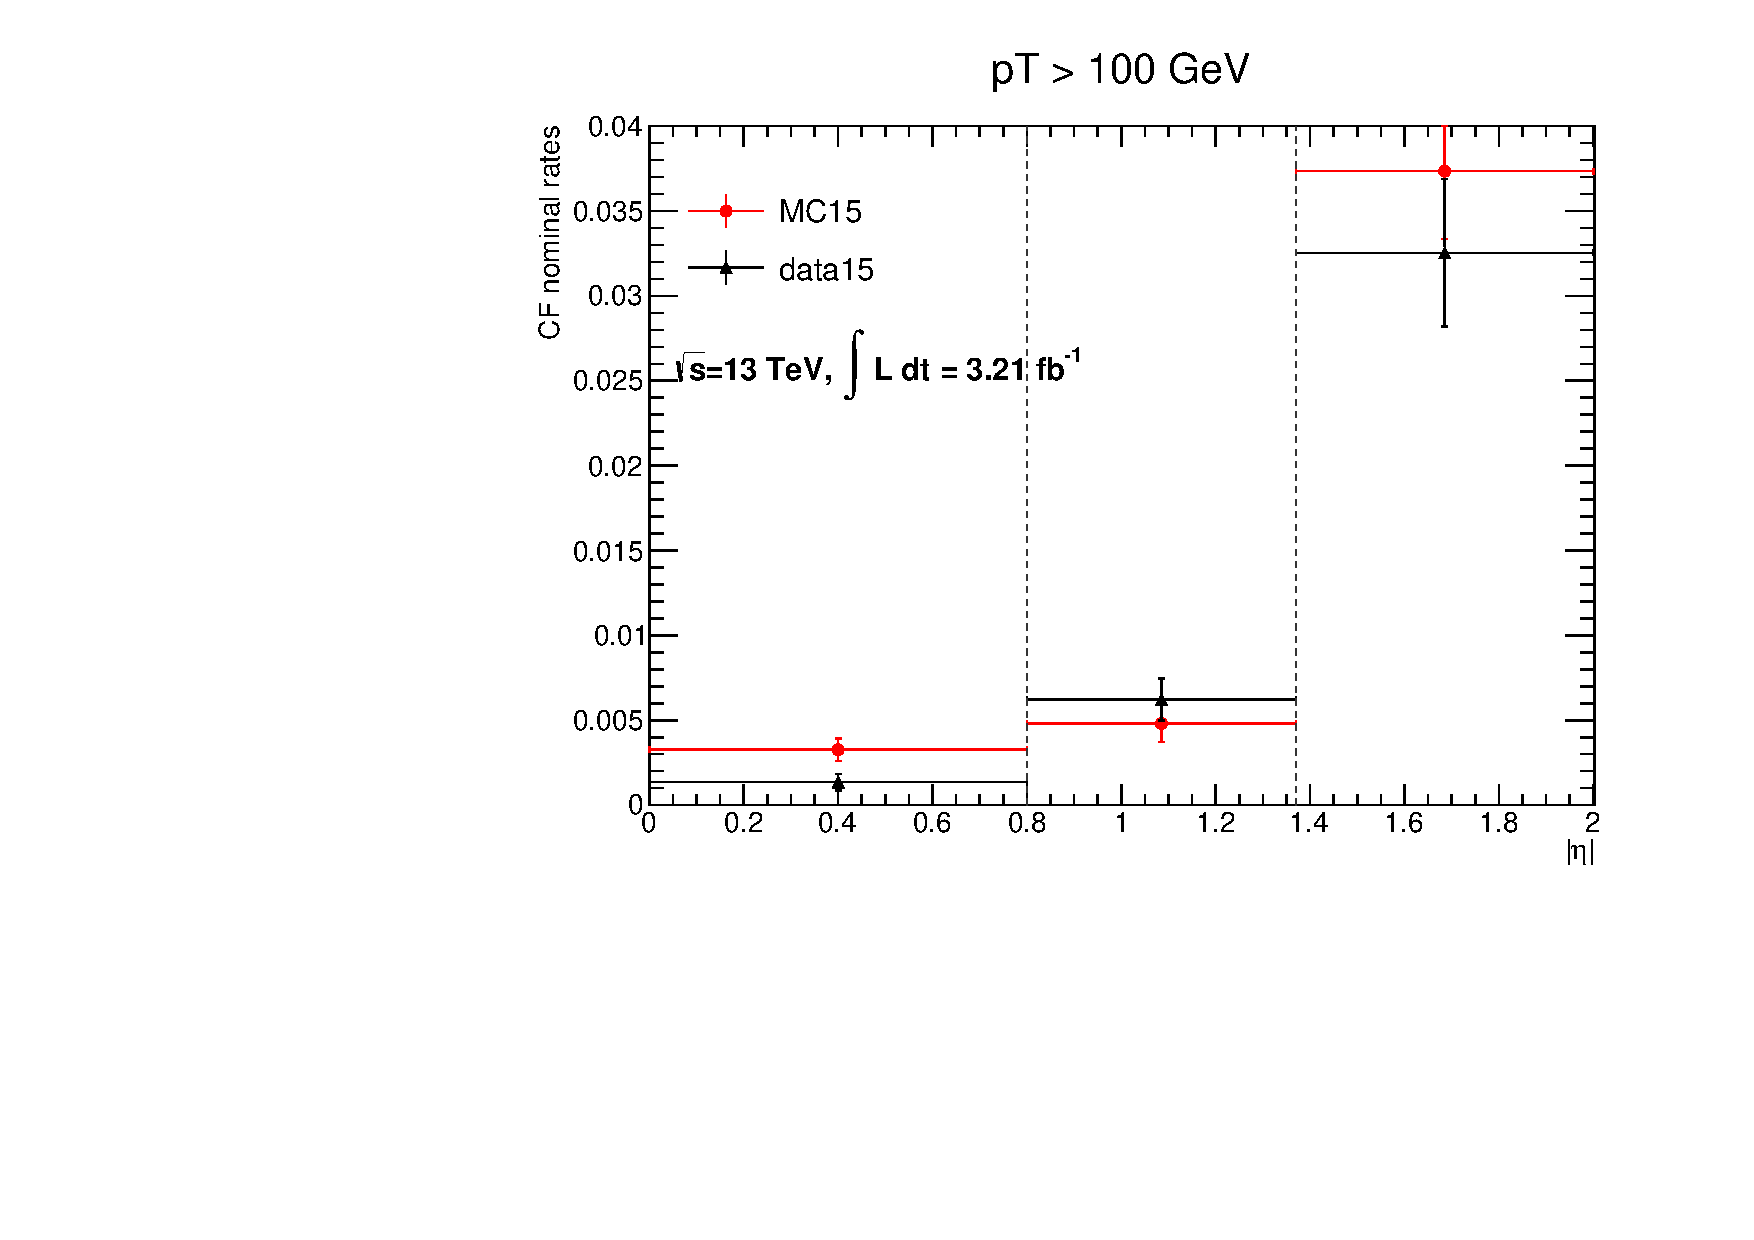
\includegraphics[width=0.4\textwidth]{FIGURES/BKG/chargeFlip/CFrates___dataVSmc___PTbin9.pdf}
\caption{\label{fig:CFratesNominal_1} Charge flip rates extracted from data (black dots) and from MC $Z\to e^+e^-$ (red dots) for electrons satisfying the signal requirements, as a function of $\eta$ and in various $\pt$ bins. Statistical and systematic uncertainties are shown.}
\end{figure}
%------------------------------------------------


%------------------------------------------------
\begin{figure}[h!]
\centering
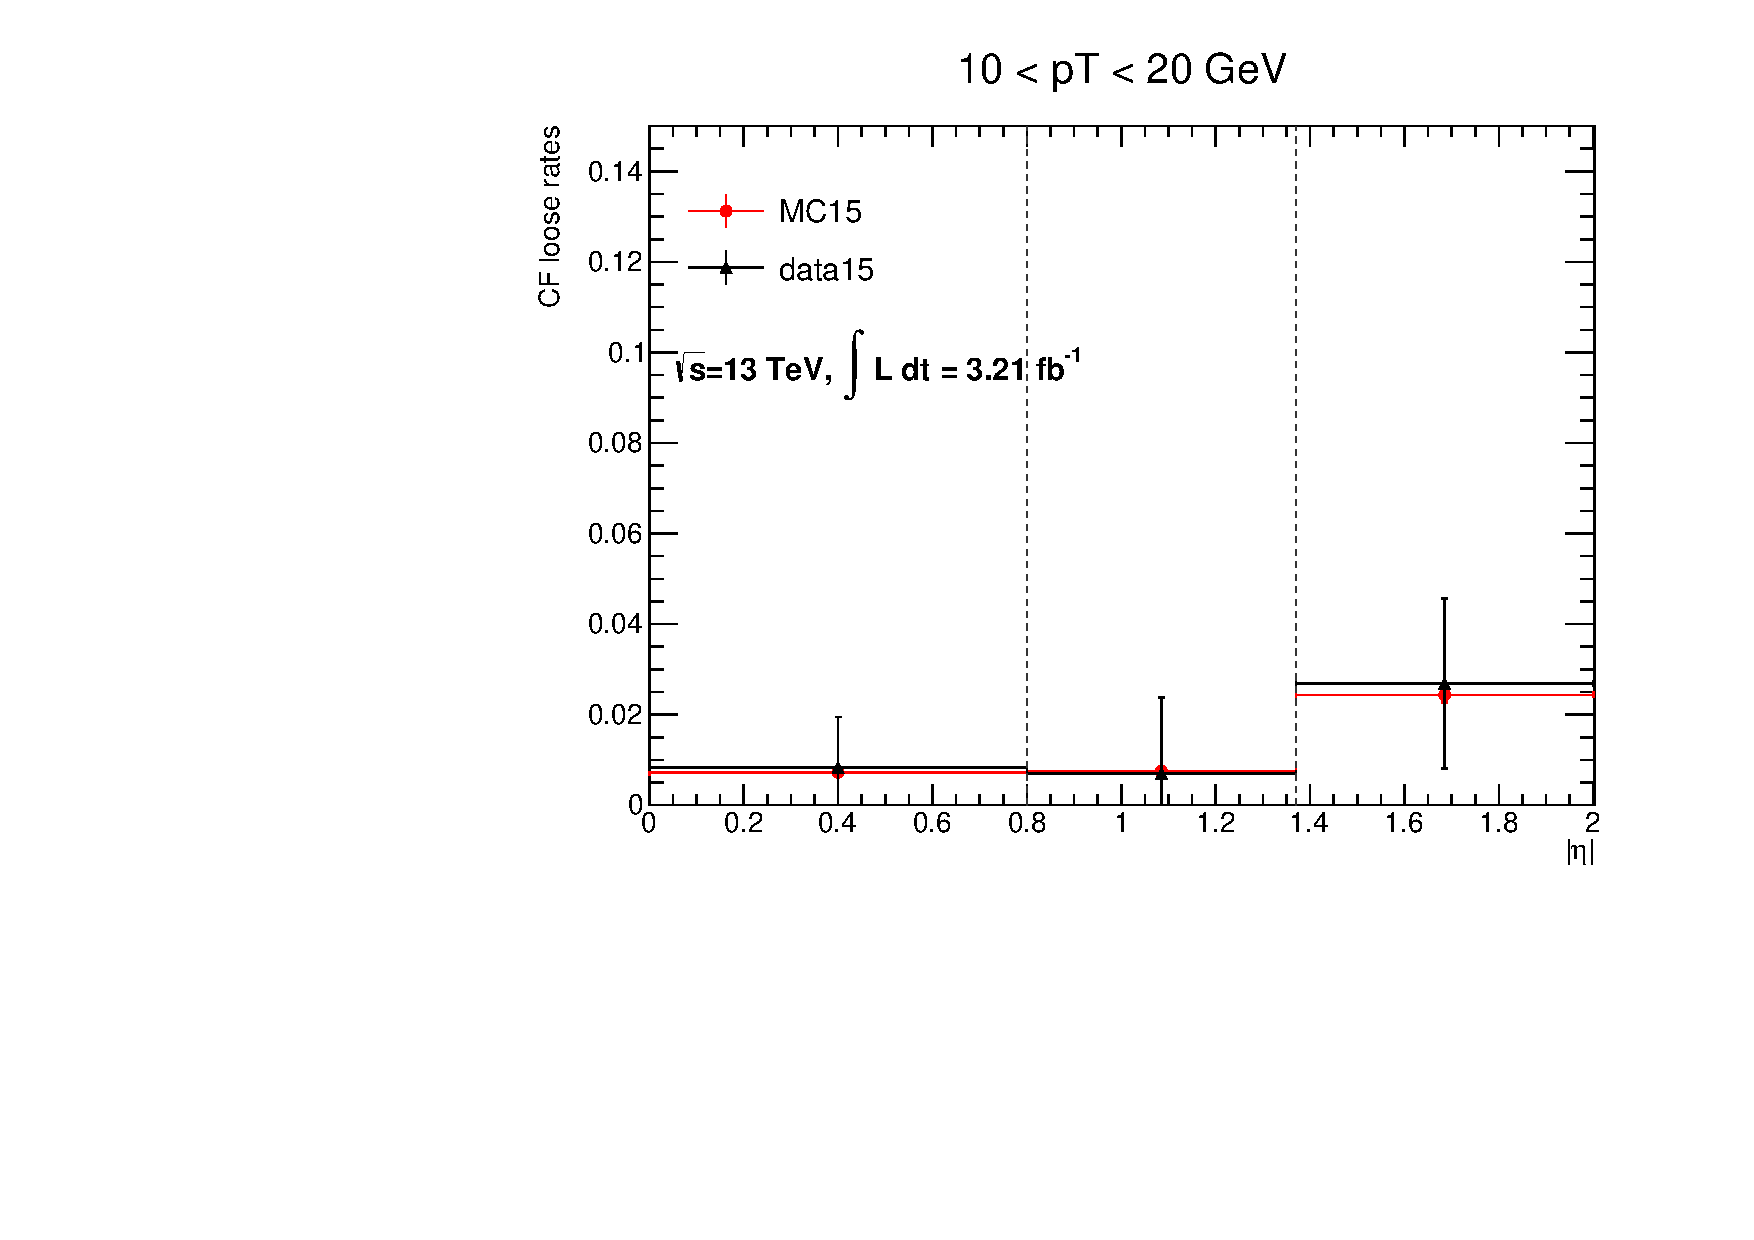
\includegraphics[width=0.4\textwidth]{FIGURES/BKG/chargeFlip/CFratesLOOSE___dataVSmc___PTbin0.pdf}
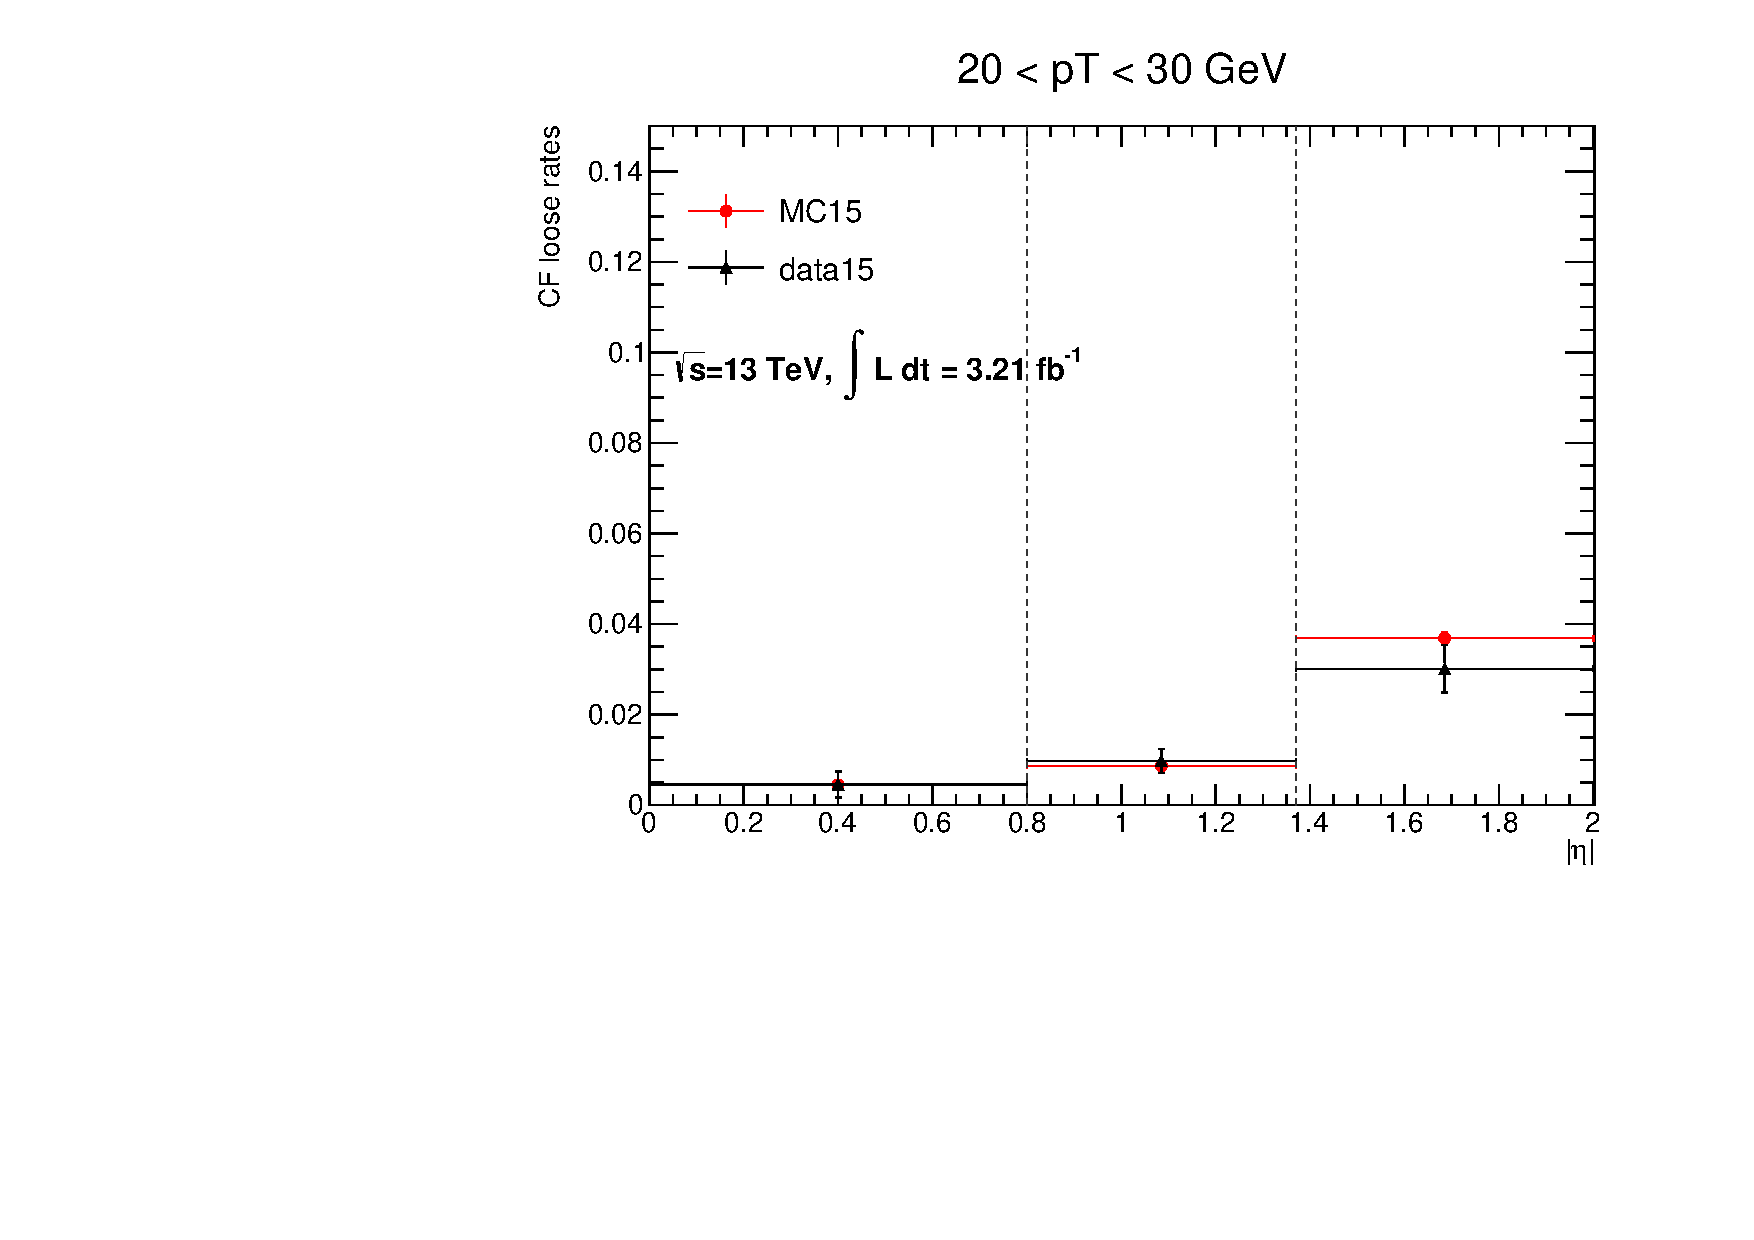
\includegraphics[width=0.4\textwidth]{FIGURES/BKG/chargeFlip/CFratesLOOSE___dataVSmc___PTbin1.pdf}
\vfill
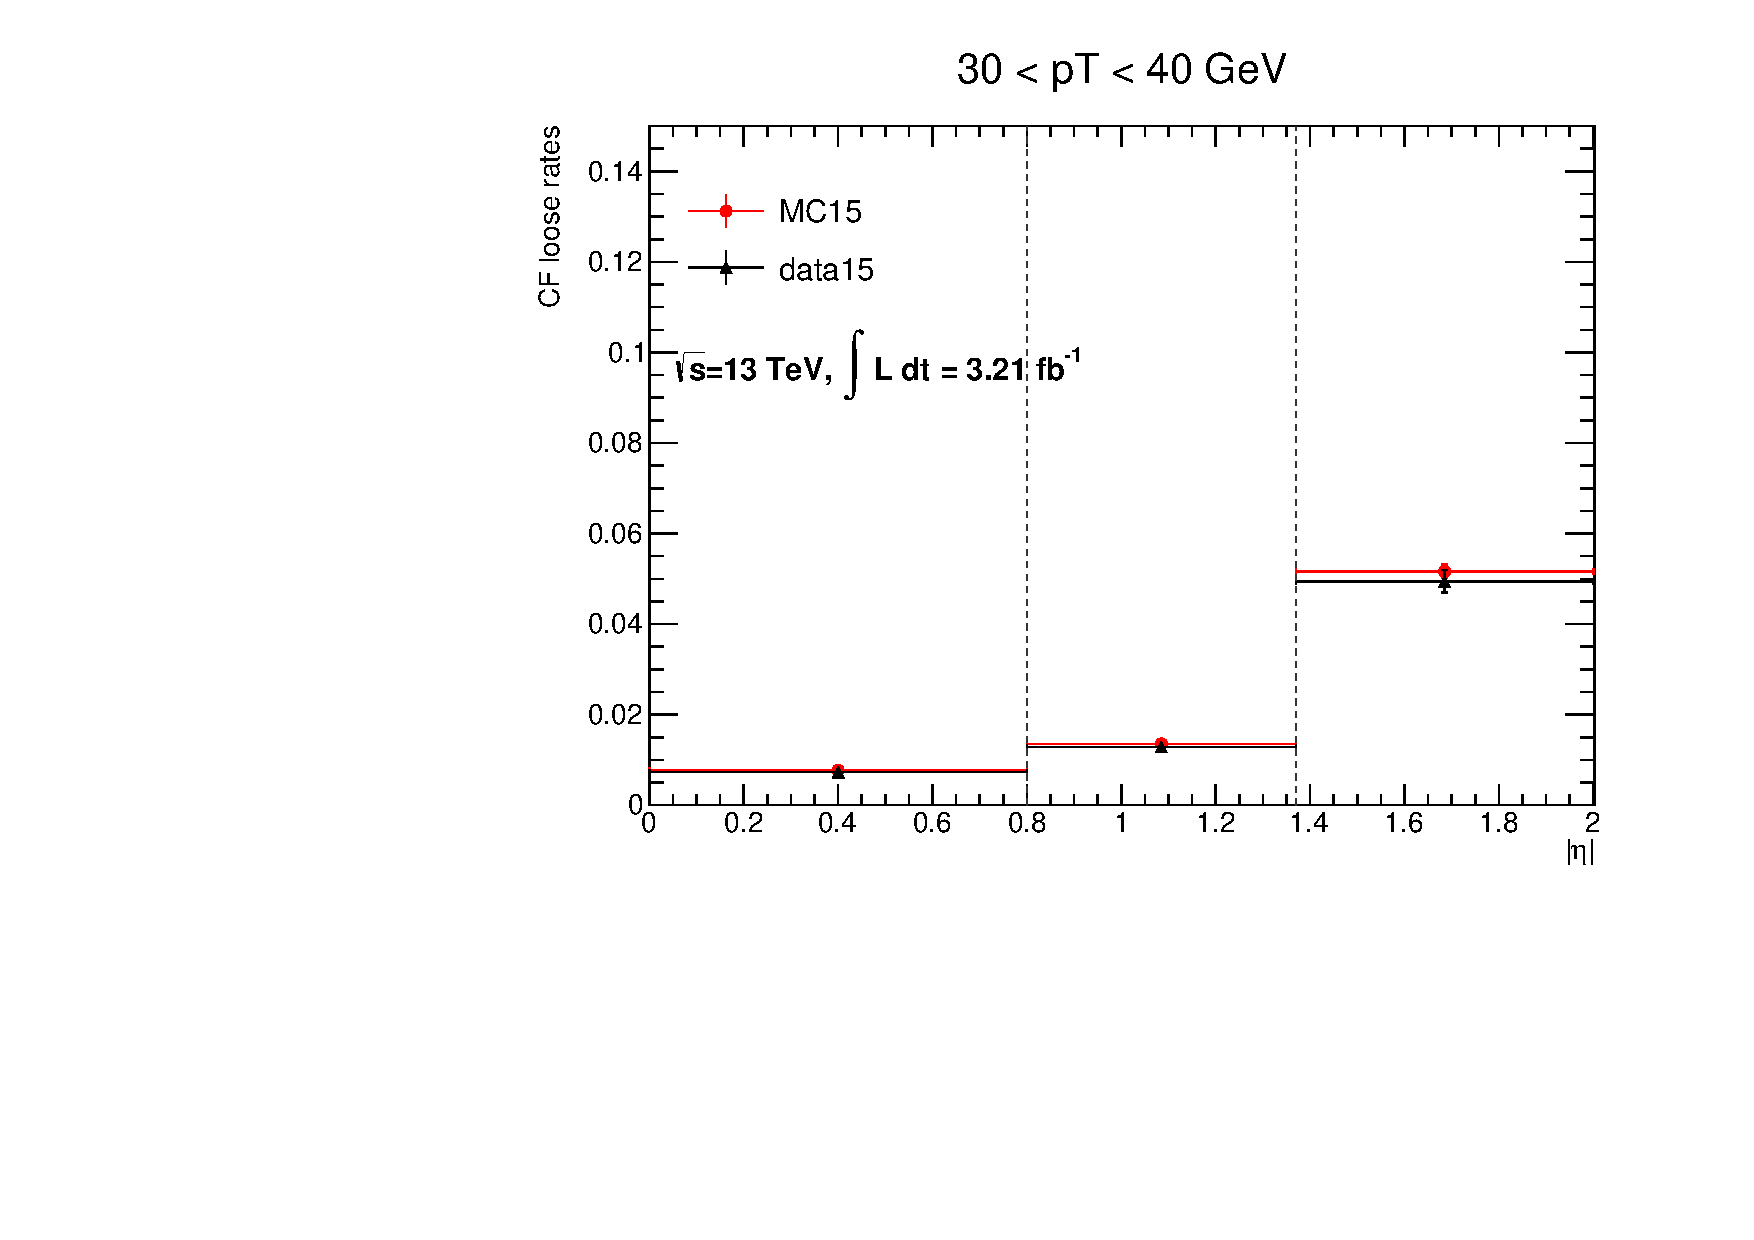
\includegraphics[width=0.4\textwidth]{FIGURES/BKG/chargeFlip/CFratesLOOSE___dataVSmc___PTbin2.pdf}
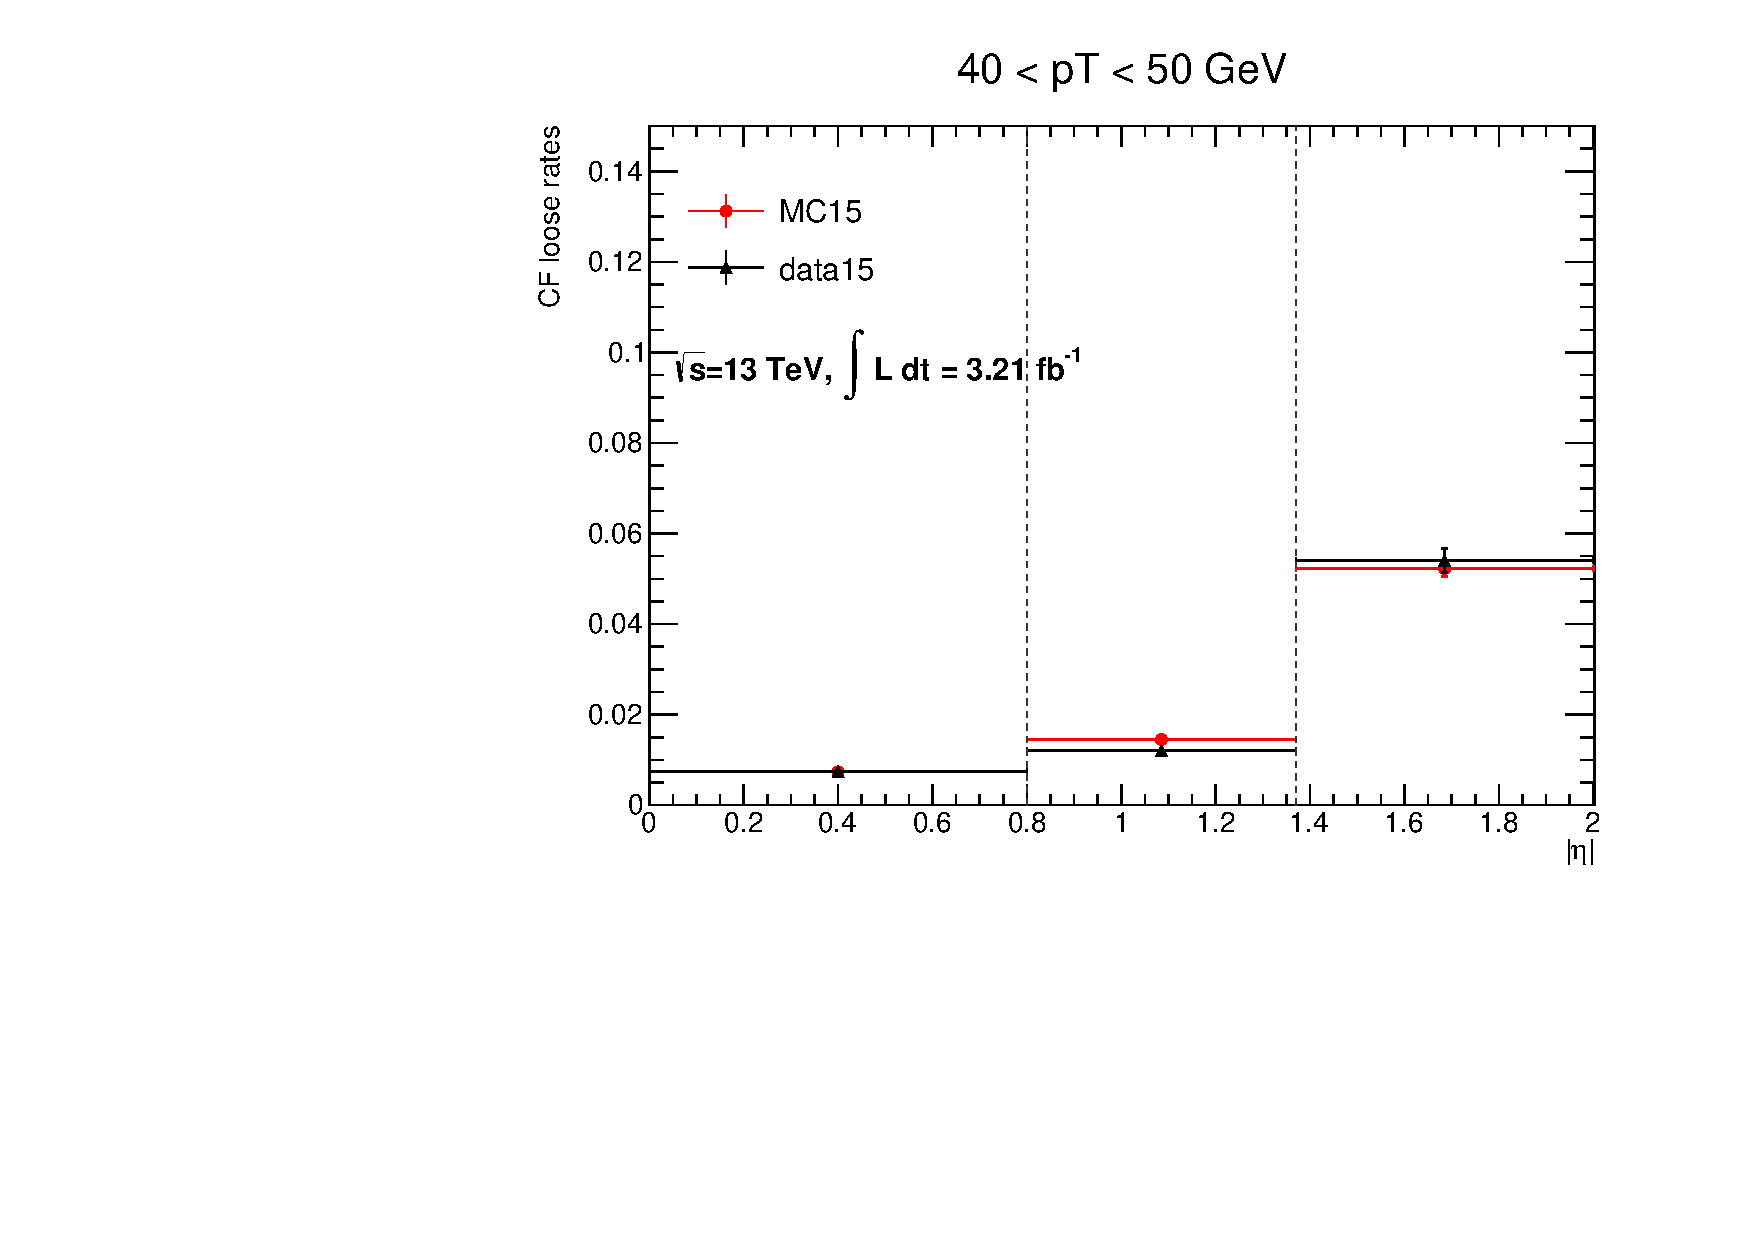
\includegraphics[width=0.4\textwidth]{FIGURES/BKG/chargeFlip/CFratesLOOSE___dataVSmc___PTbin3.pdf}

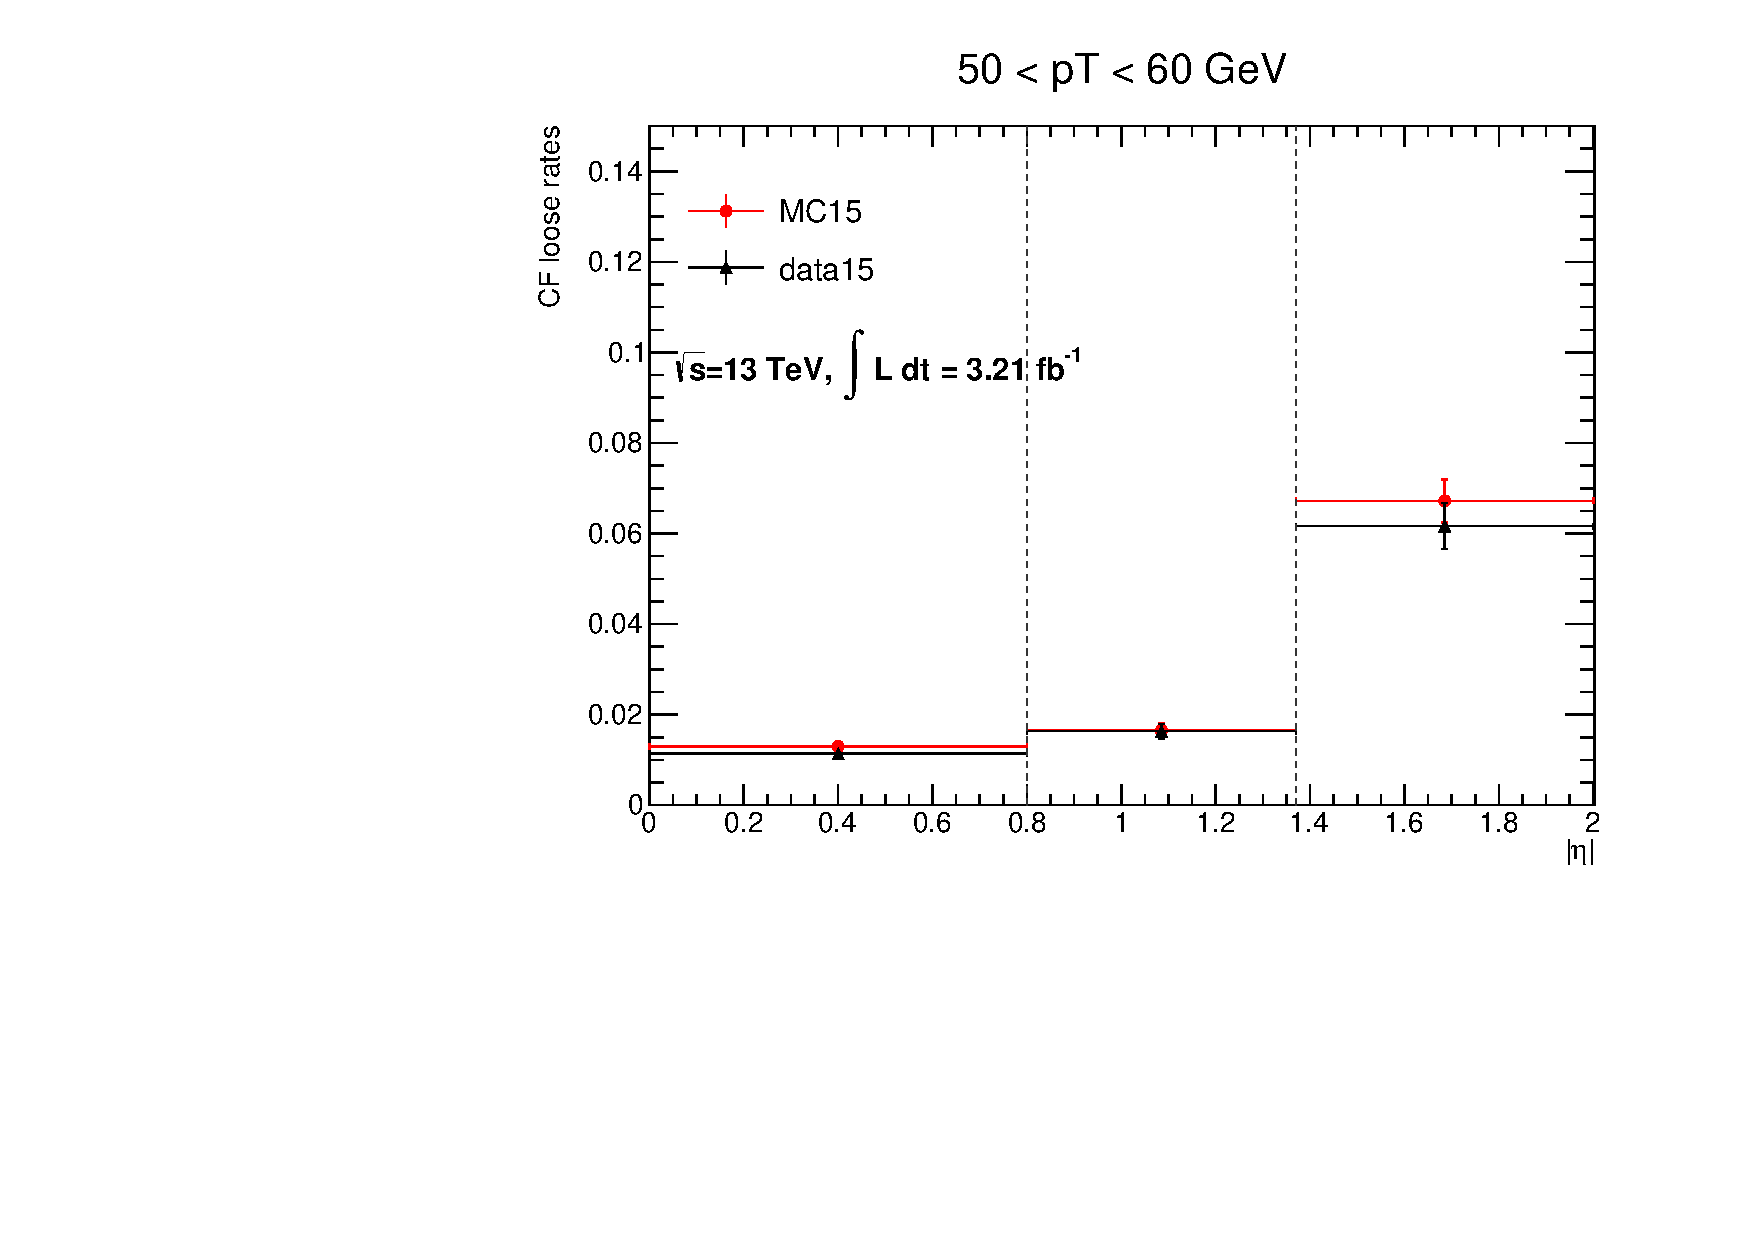
\includegraphics[width=0.4\textwidth]{FIGURES/BKG/chargeFlip/CFratesLOOSE___dataVSmc___PTbin4.pdf}
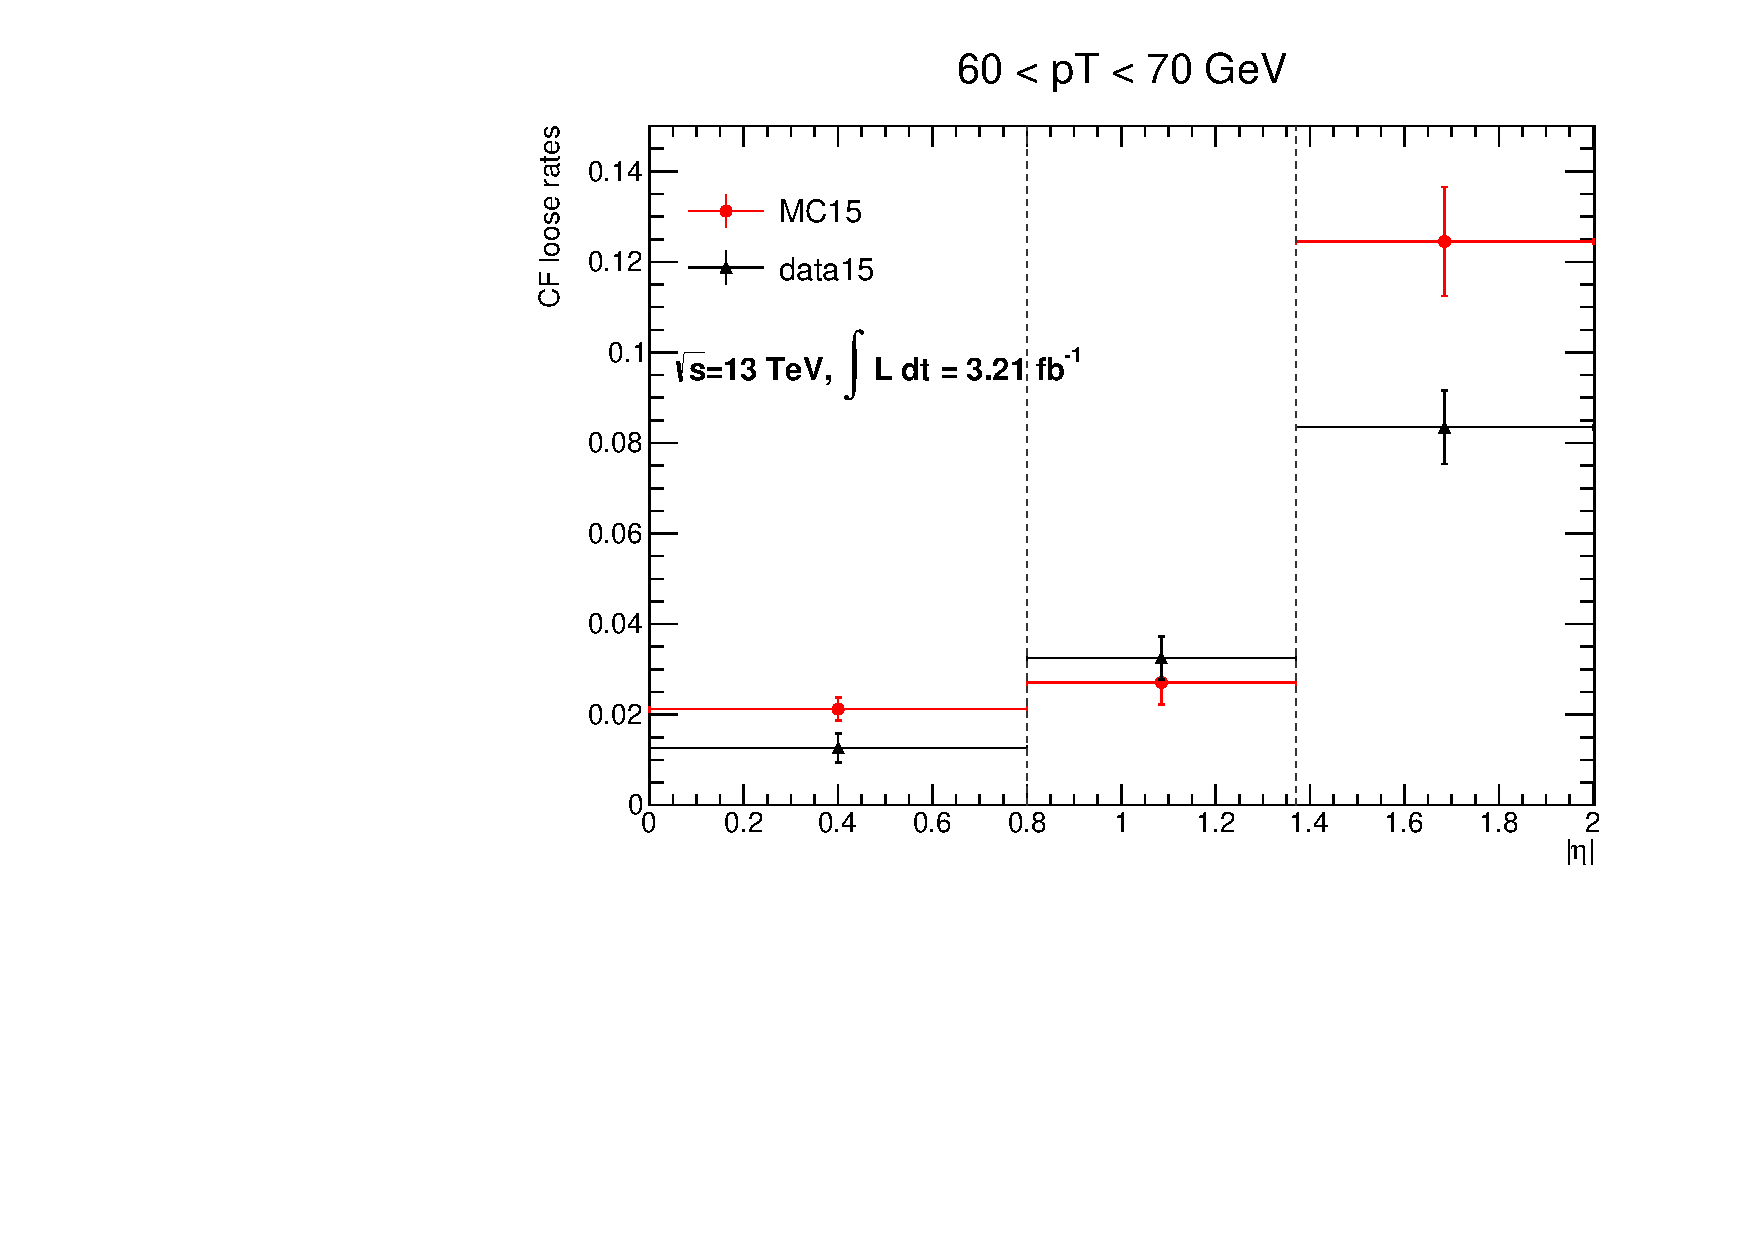
\includegraphics[width=0.4\textwidth]{FIGURES/BKG/chargeFlip/CFratesLOOSE___dataVSmc___PTbin5.pdf}
\vfill
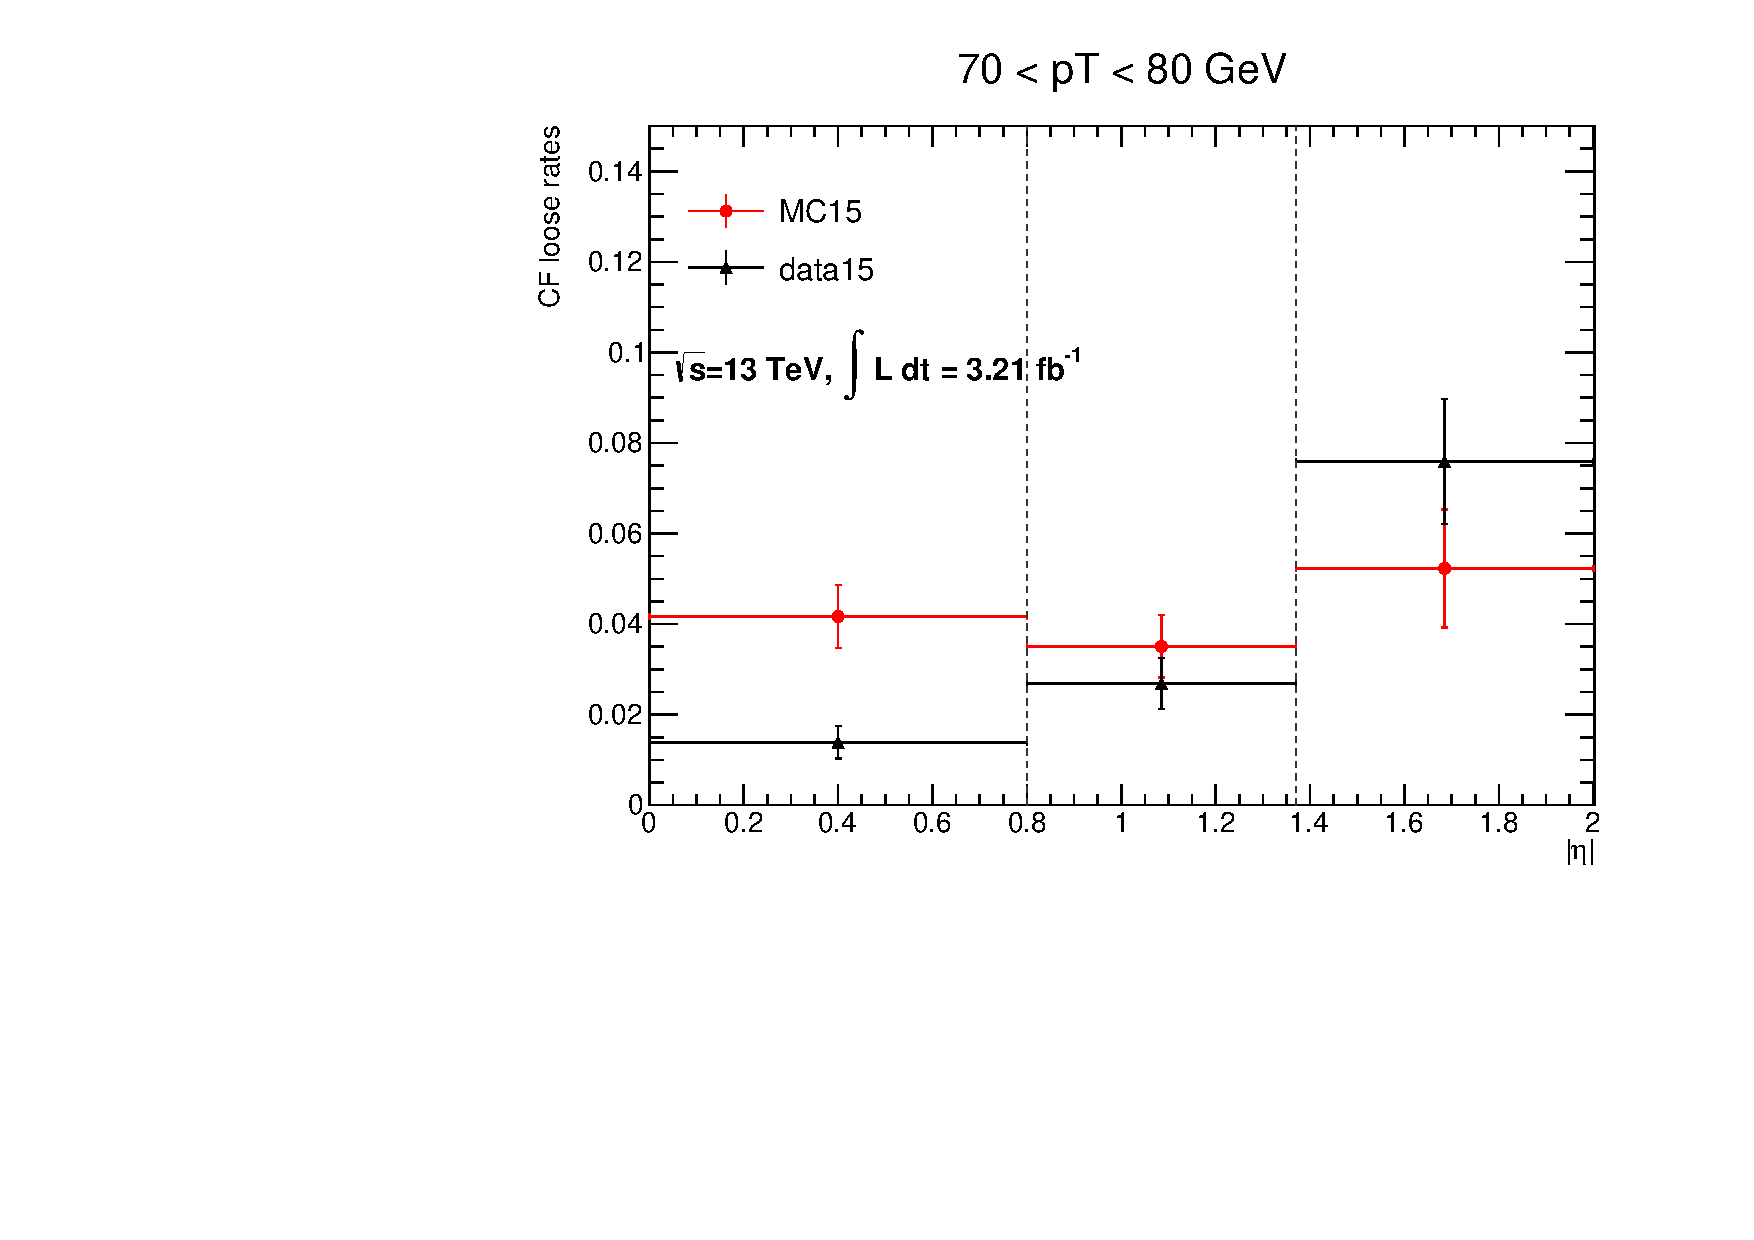
\includegraphics[width=0.4\textwidth]{FIGURES/BKG/chargeFlip/CFratesLOOSE___dataVSmc___PTbin6.pdf}
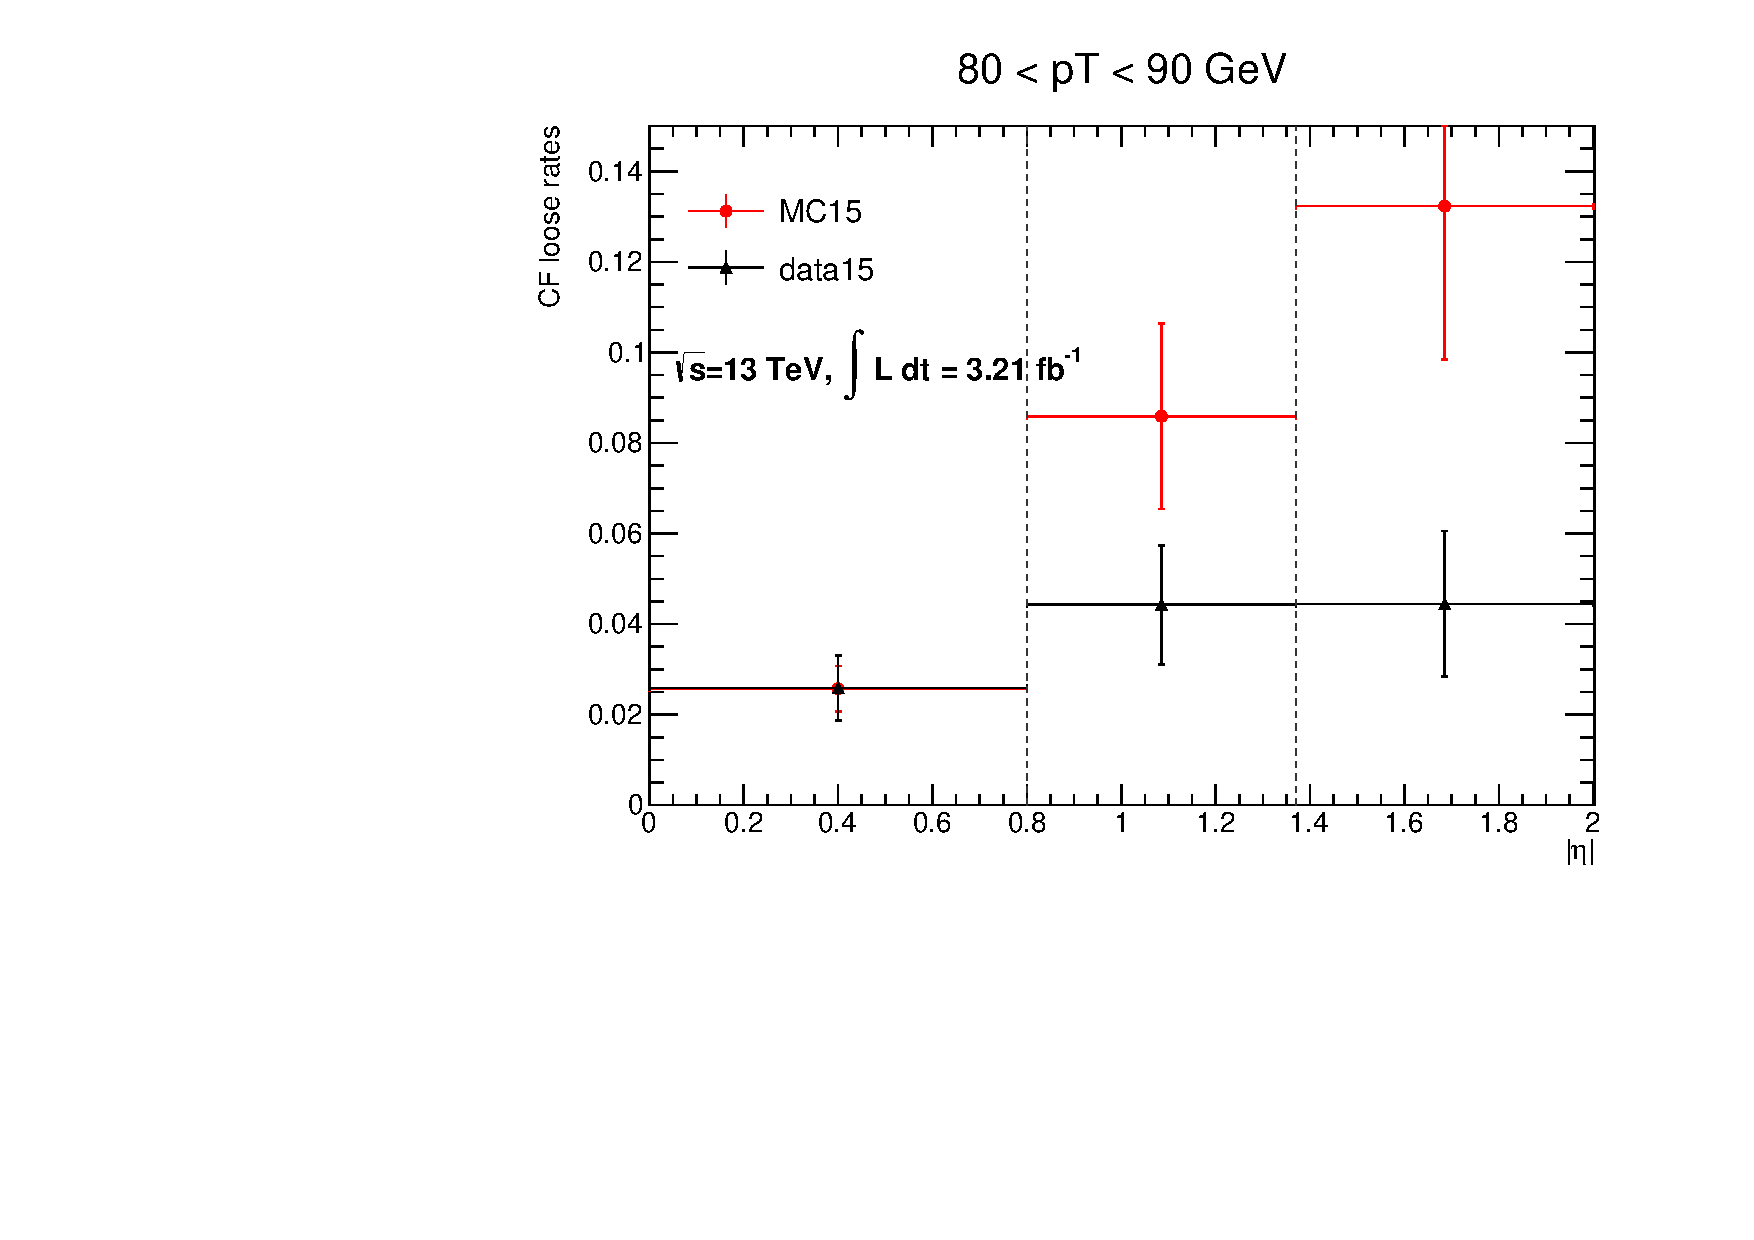
\includegraphics[width=0.4\textwidth]{FIGURES/BKG/chargeFlip/CFratesLOOSE___dataVSmc___PTbin7.pdf}
\vfill
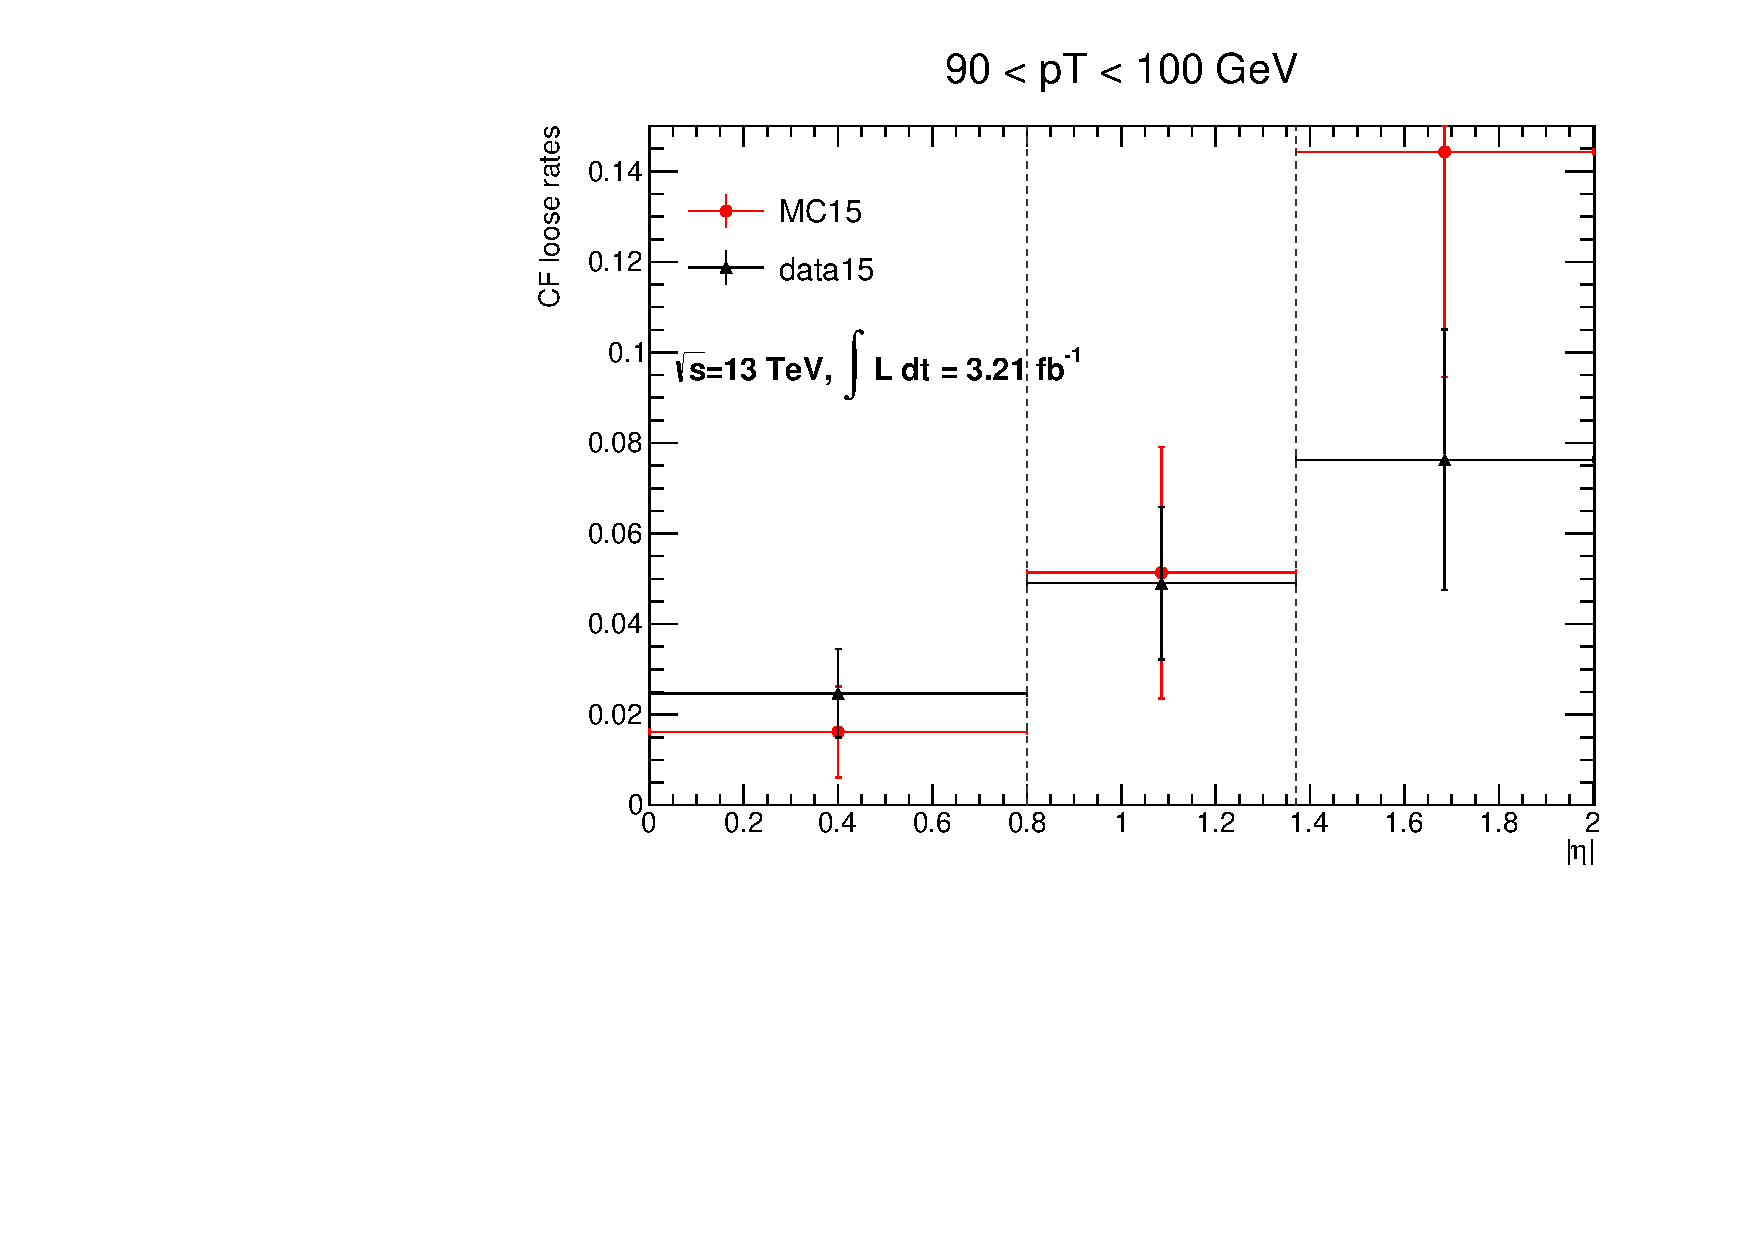
\includegraphics[width=0.4\textwidth]{FIGURES/BKG/chargeFlip/CFratesLOOSE___dataVSmc___PTbin8.pdf}
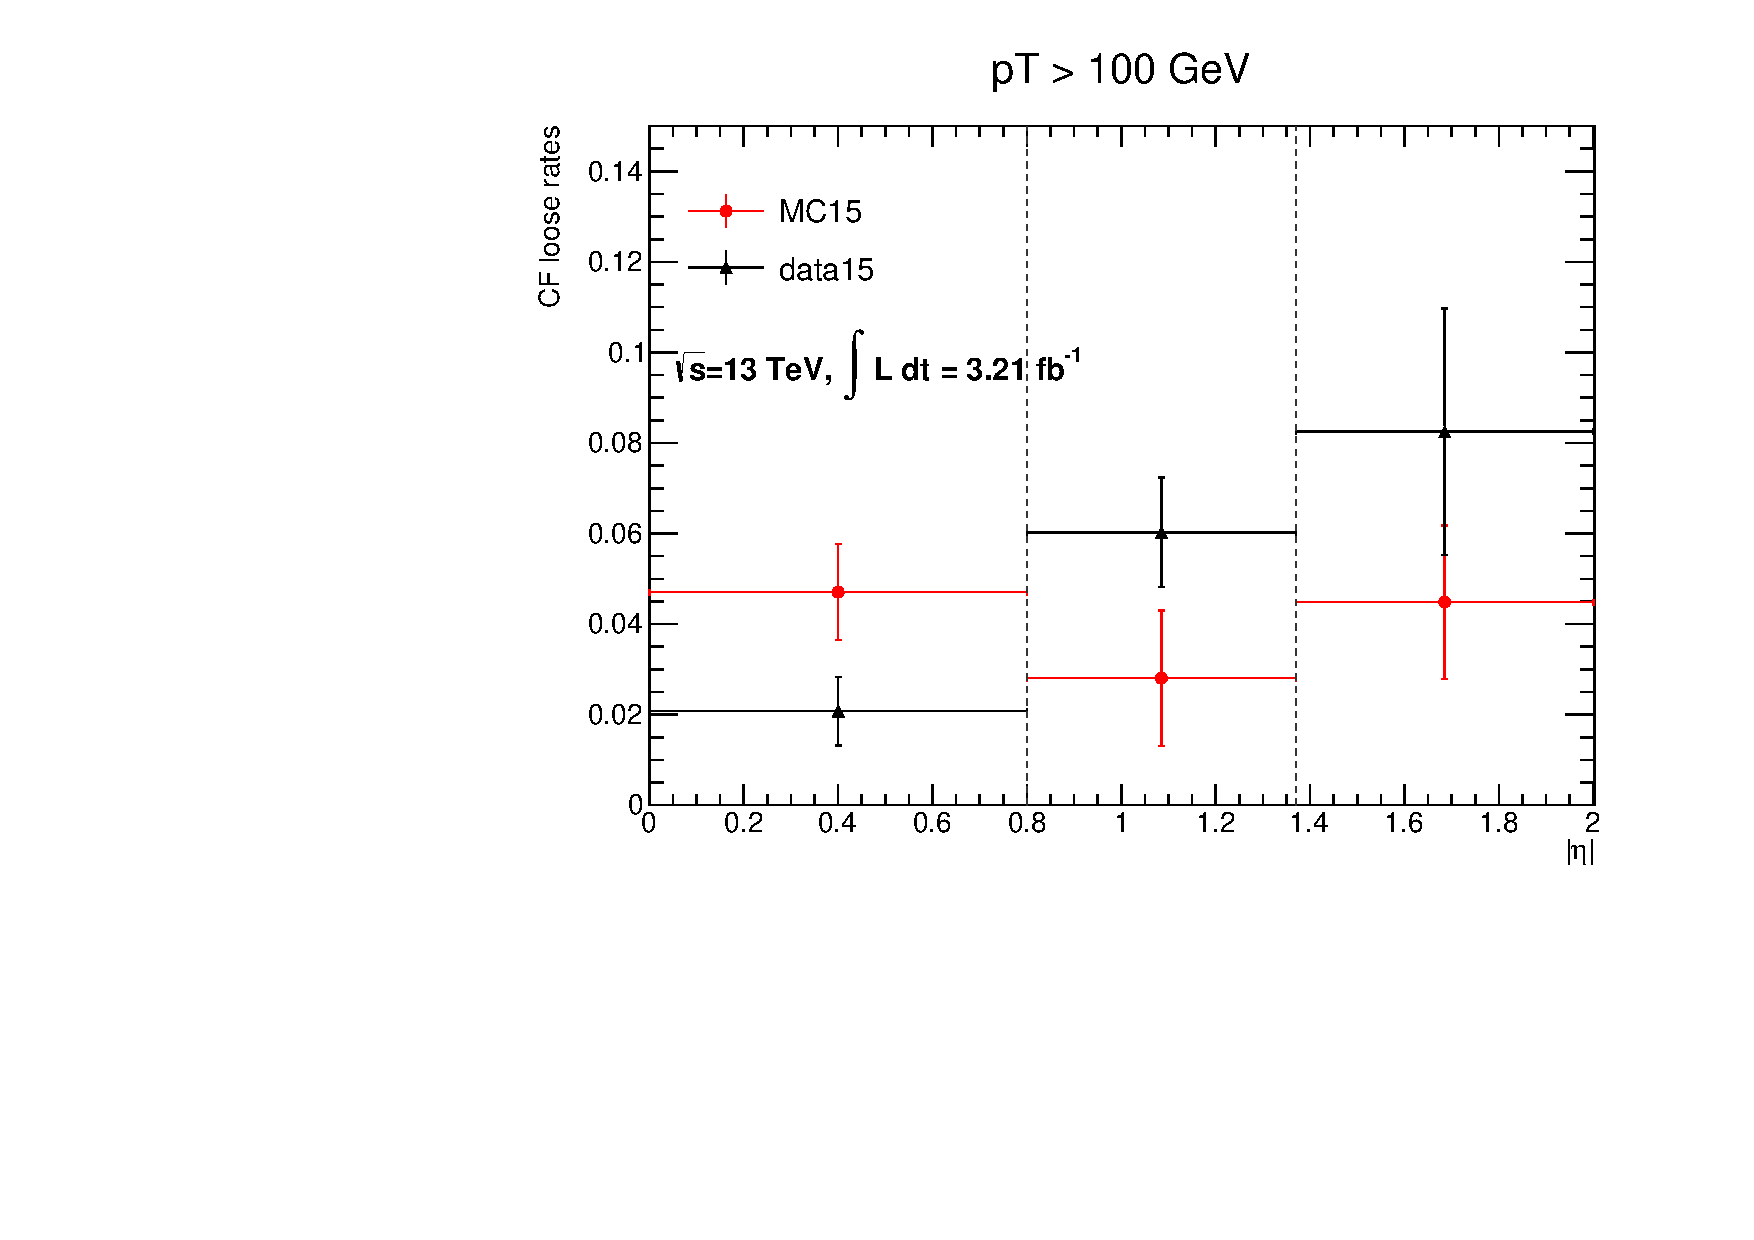
\includegraphics[width=0.4\textwidth]{FIGURES/BKG/chargeFlip/CFratesLOOSE___dataVSmc___PTbin9.pdf}
\caption{\label{fig:CFratesLoose_2} Charge flip rates extracted from data (black dots) and from MC $Z\to e^+e^-$ (red dots) for electrons failing the signal requirements, as a function of $\eta$ and in various $\pt$ bins. Statistical and systematic uncertainties are shown.}
\end{figure}
%------------------------------------------------
%\FloatBarrier


\subsubsection{Systematics}
\label{subsec:CFsysSection}

The uncertainties on the charge mis-identification rates coming from the background subtraction procedure are computed and assigned as systematics. As mentioned in the previous section, the standard measurement is computed using a central-band width of $75<m_{ee}<100$~GeV and side-band regions of 25~GeV for the background subtraction. To evaluate the systematics, the charge flip rates were extracted for five different configurations: 
\begin{enumerate}
\item $75<m_{ee}<100$~GeV, no background subtraction; 
\item $75<m_{ee}<100$~GeV, side-band of 20~GeV;
\item $75<m_{ee}<100$~GeV, side-band of 25~GeV (standard measurement);
\item $75<m_{ee}<100$~GeV, side-band of 30~GeV; 
\item $80<m_{ee}<110$ GeV GeV, side-band of 25 GeV
\end{enumerate}
We then extract four different variations by comparing those five configurations. The effect of applying the background subtraction itself (called background ON and OFF) is computed by comparing configurations 1 vs. 3. The Z mass window width effects are computed by comparing configurations 3 vs. 5, while the side-band width effects are calculated by comparing configuration 3 vs. 2 and 3 vs. 4. Then the largest deviation in each bins is taken as the systematic uncertainty on the charge flip rates. 

Those variations are shown on Figure~\ref{fig:CFsys} for a $\pt$ range of 20-30 GeV for both type of events where electrons satisfied the signal requirements on left and where electrons don't satisfied the signal requirements (auxiliary measurement) on right. The black dots represent the standard measurement and coloured dots represent the different configurations used to compute the systematics. Figure~\ref{fig:CFsysTot} shows the total systematic uncertainties in each $[\pt,\eta]$ bin after combining the different contributions associated to the background subtraction method. The upper plot stand for the electron passing the signal requirements while lower plot is for electrons failing the signal requirements.

\begin{figure}[htb!]
\centering
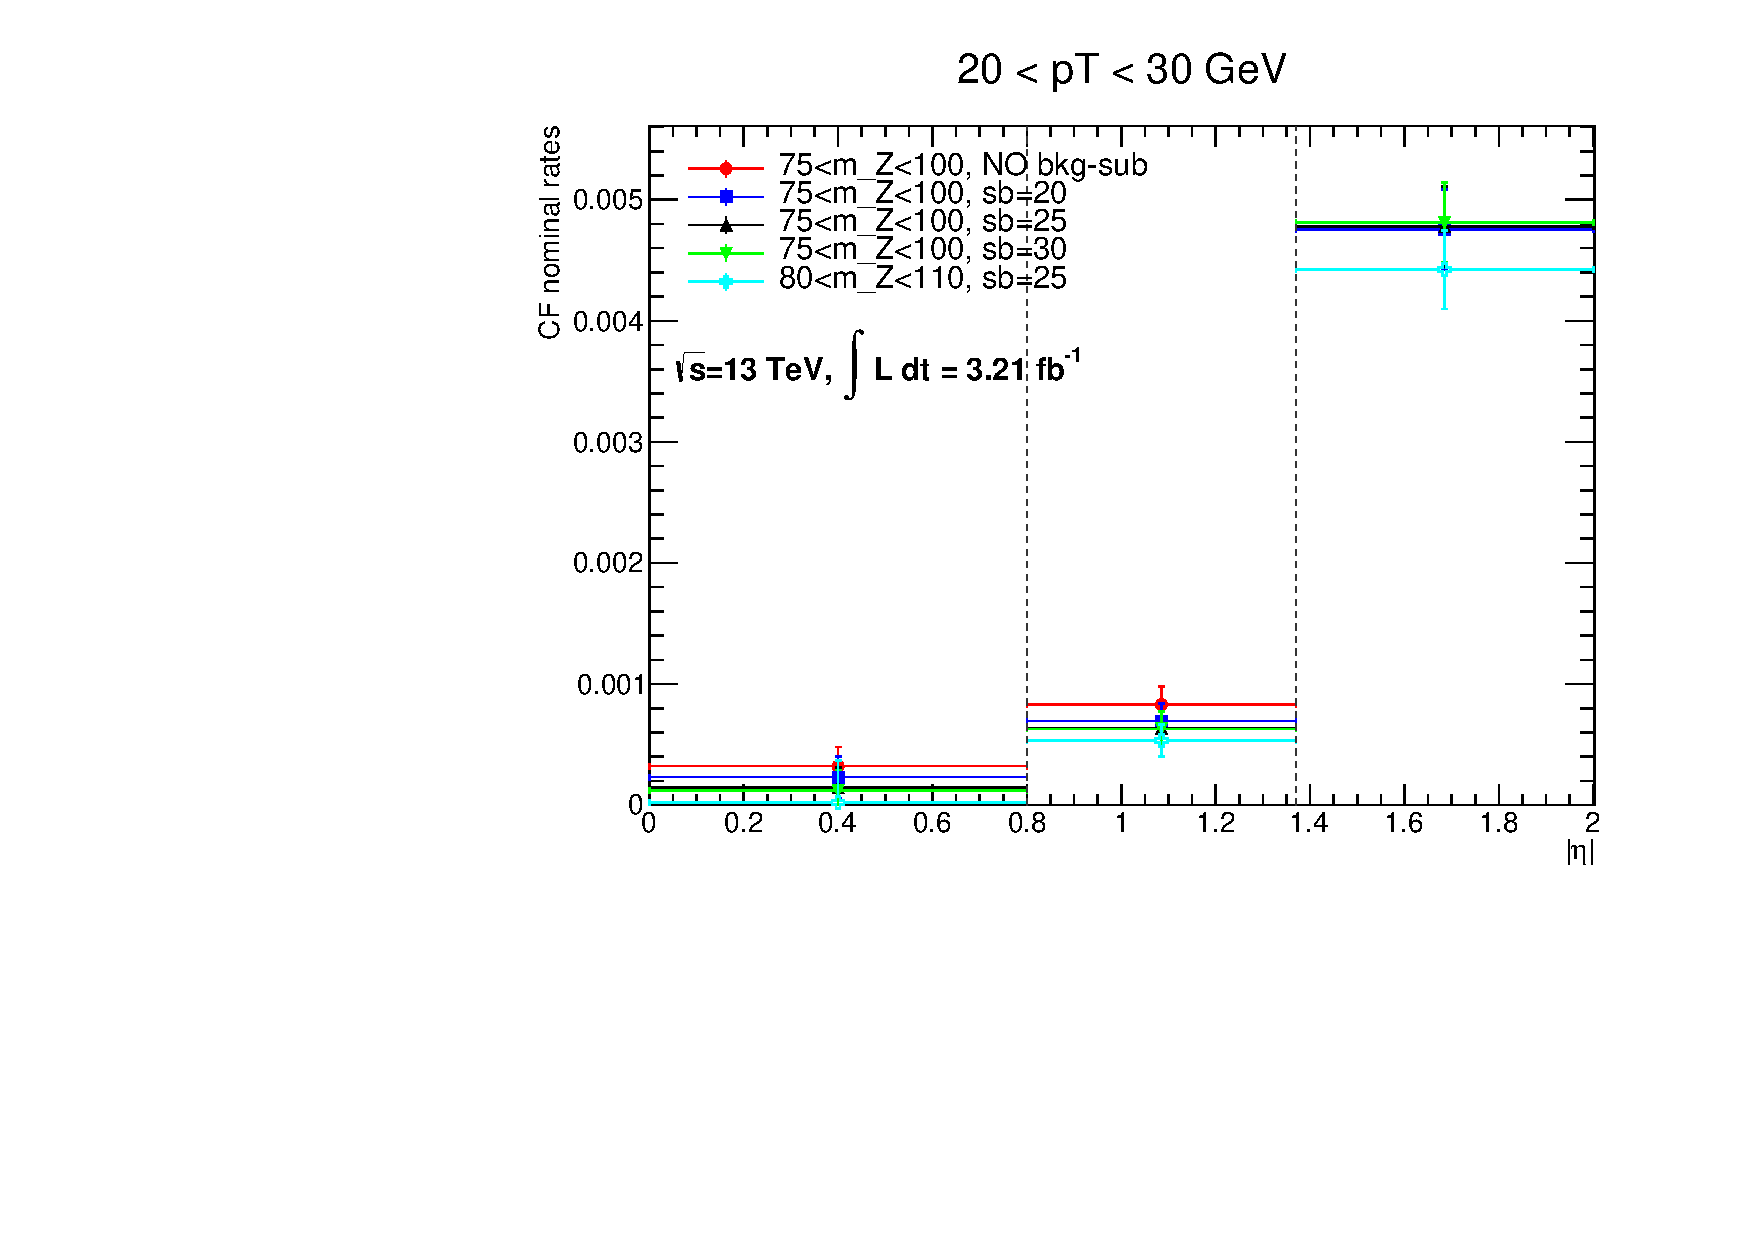
\includegraphics[width=0.48\textwidth]{FIGURES/BKG/chargeFlip/CFrates___SYStypes___PTbin1.pdf}
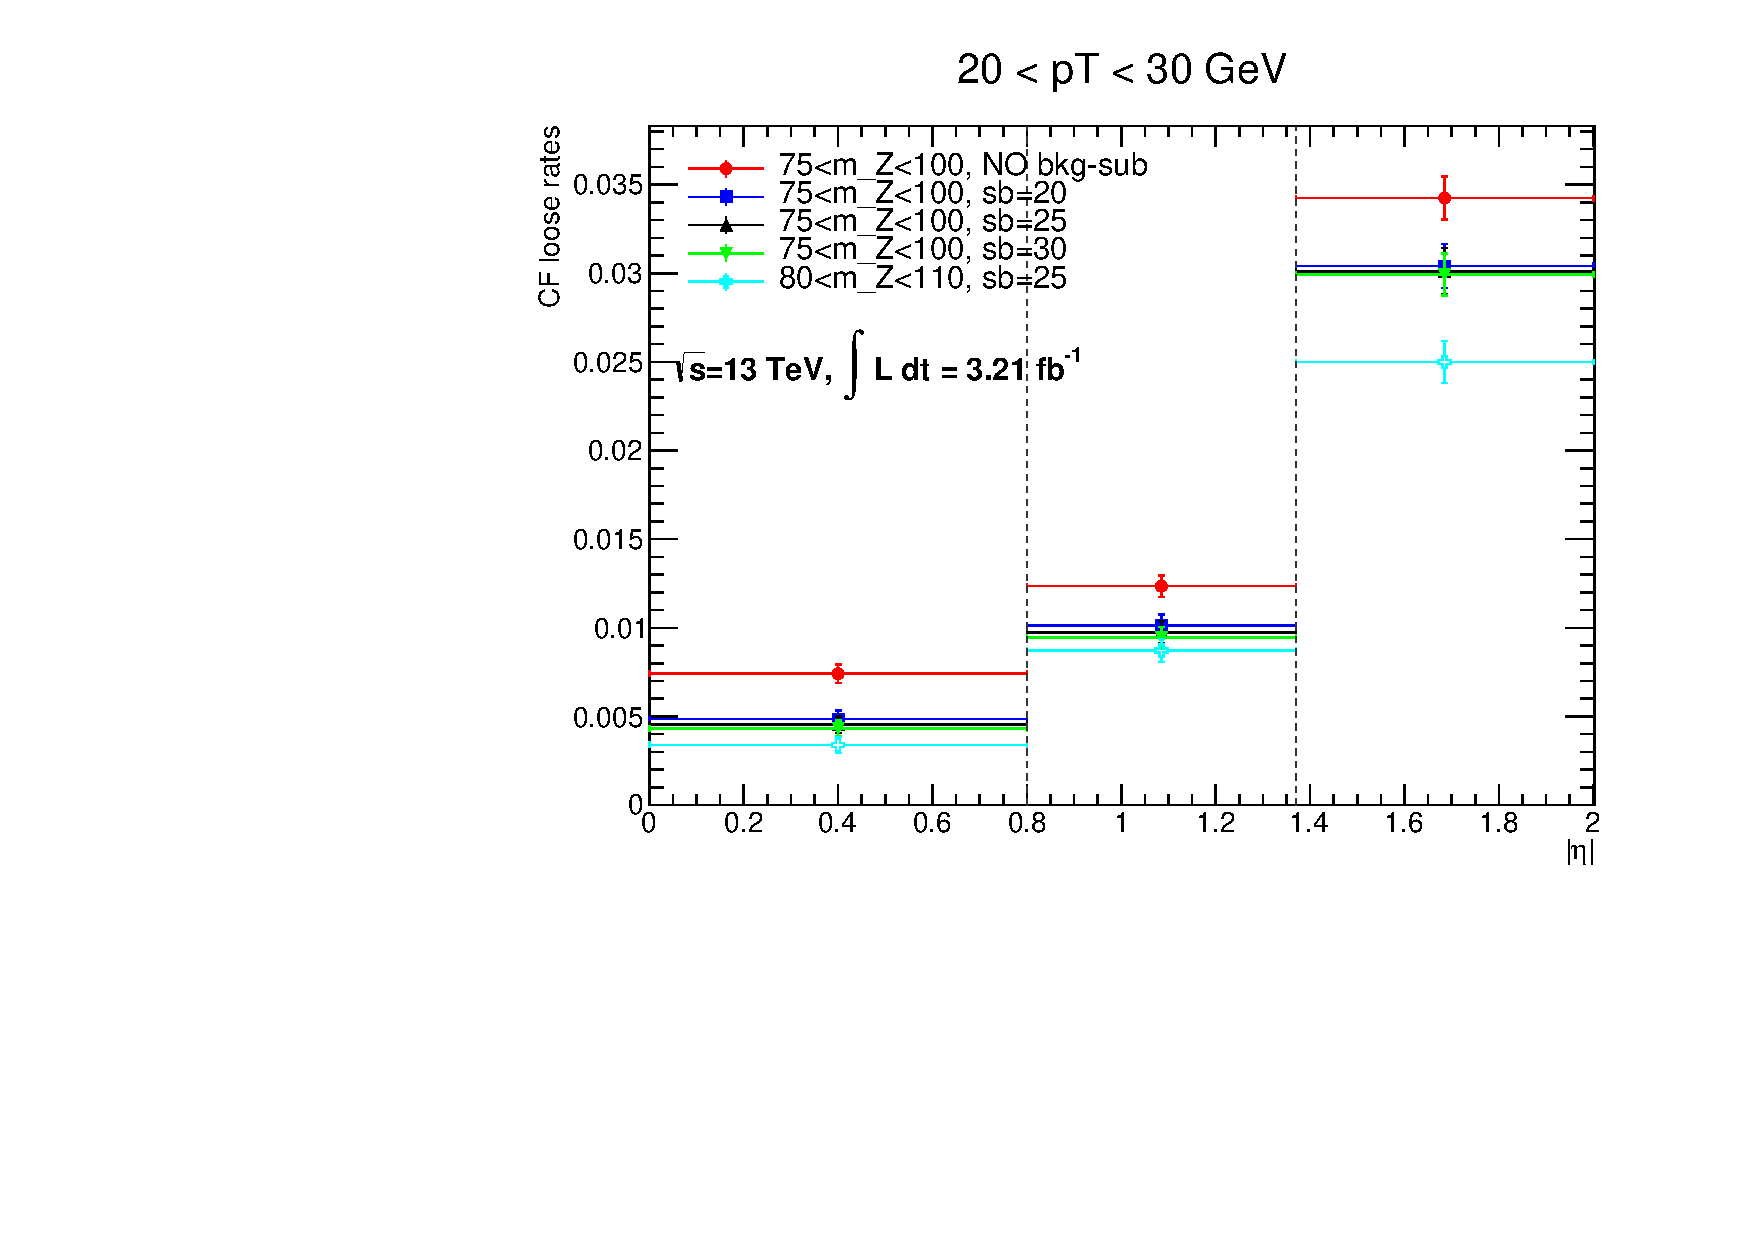
\includegraphics[width=0.48\textwidth]{FIGURES/BKG/chargeFlip/CFratesLOOSE___SYStypes___PTbin1.pdf}
\caption{\label{fig:CFsys} Charge flip rates in data for $20<\pt<30$ GeV bin using five different configurations of background subtraction for electrons satisfying the signal requirements on left handed plot and for electrons failing the signal requirements on the right handed plot. In each bin the largest deviation from the standard measurement (black dots) is taken to be the systematic uncertainty.}
\end{figure}

\begin{figure}[h!]
\centering
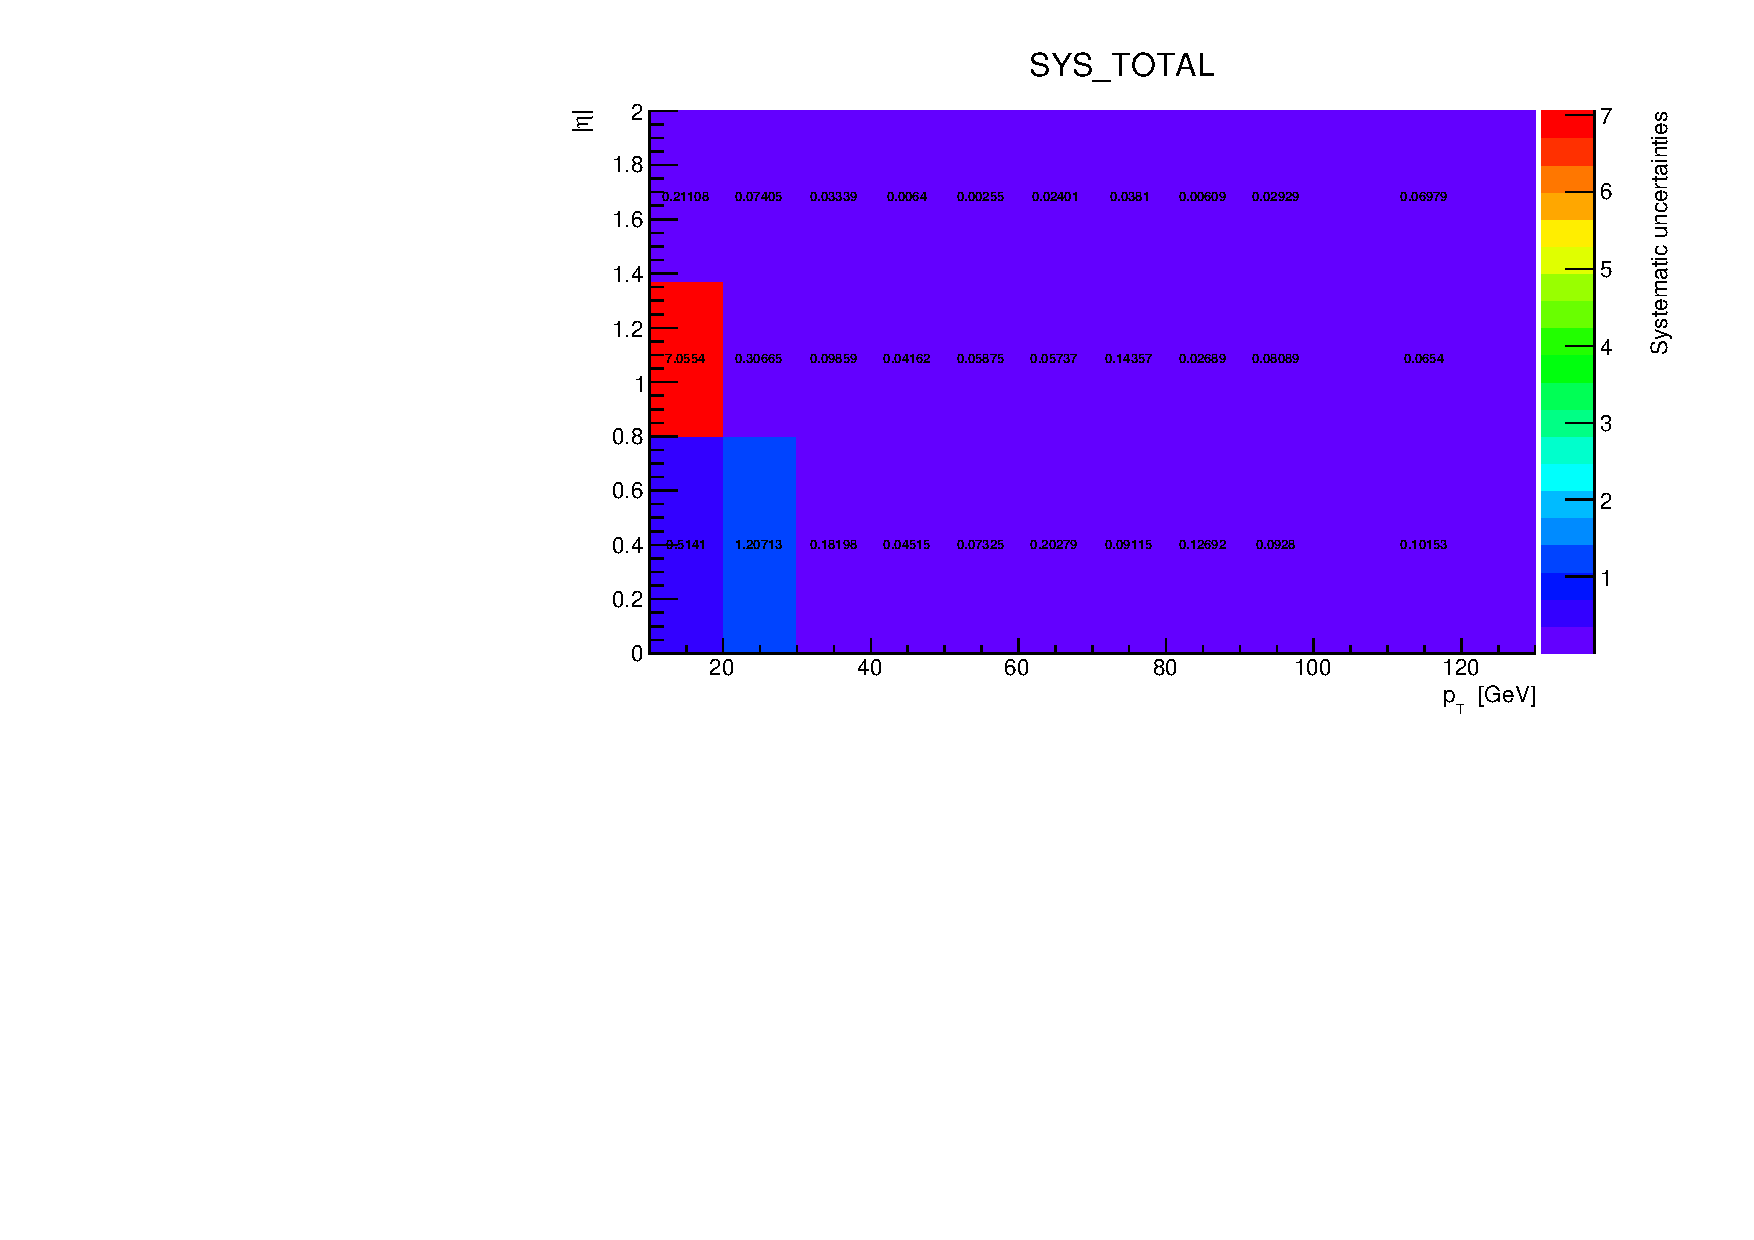
\includegraphics[width=0.65\textwidth]{FIGURES/BKG/chargeFlip/2D_histo_SYS_TOTAL.pdf}
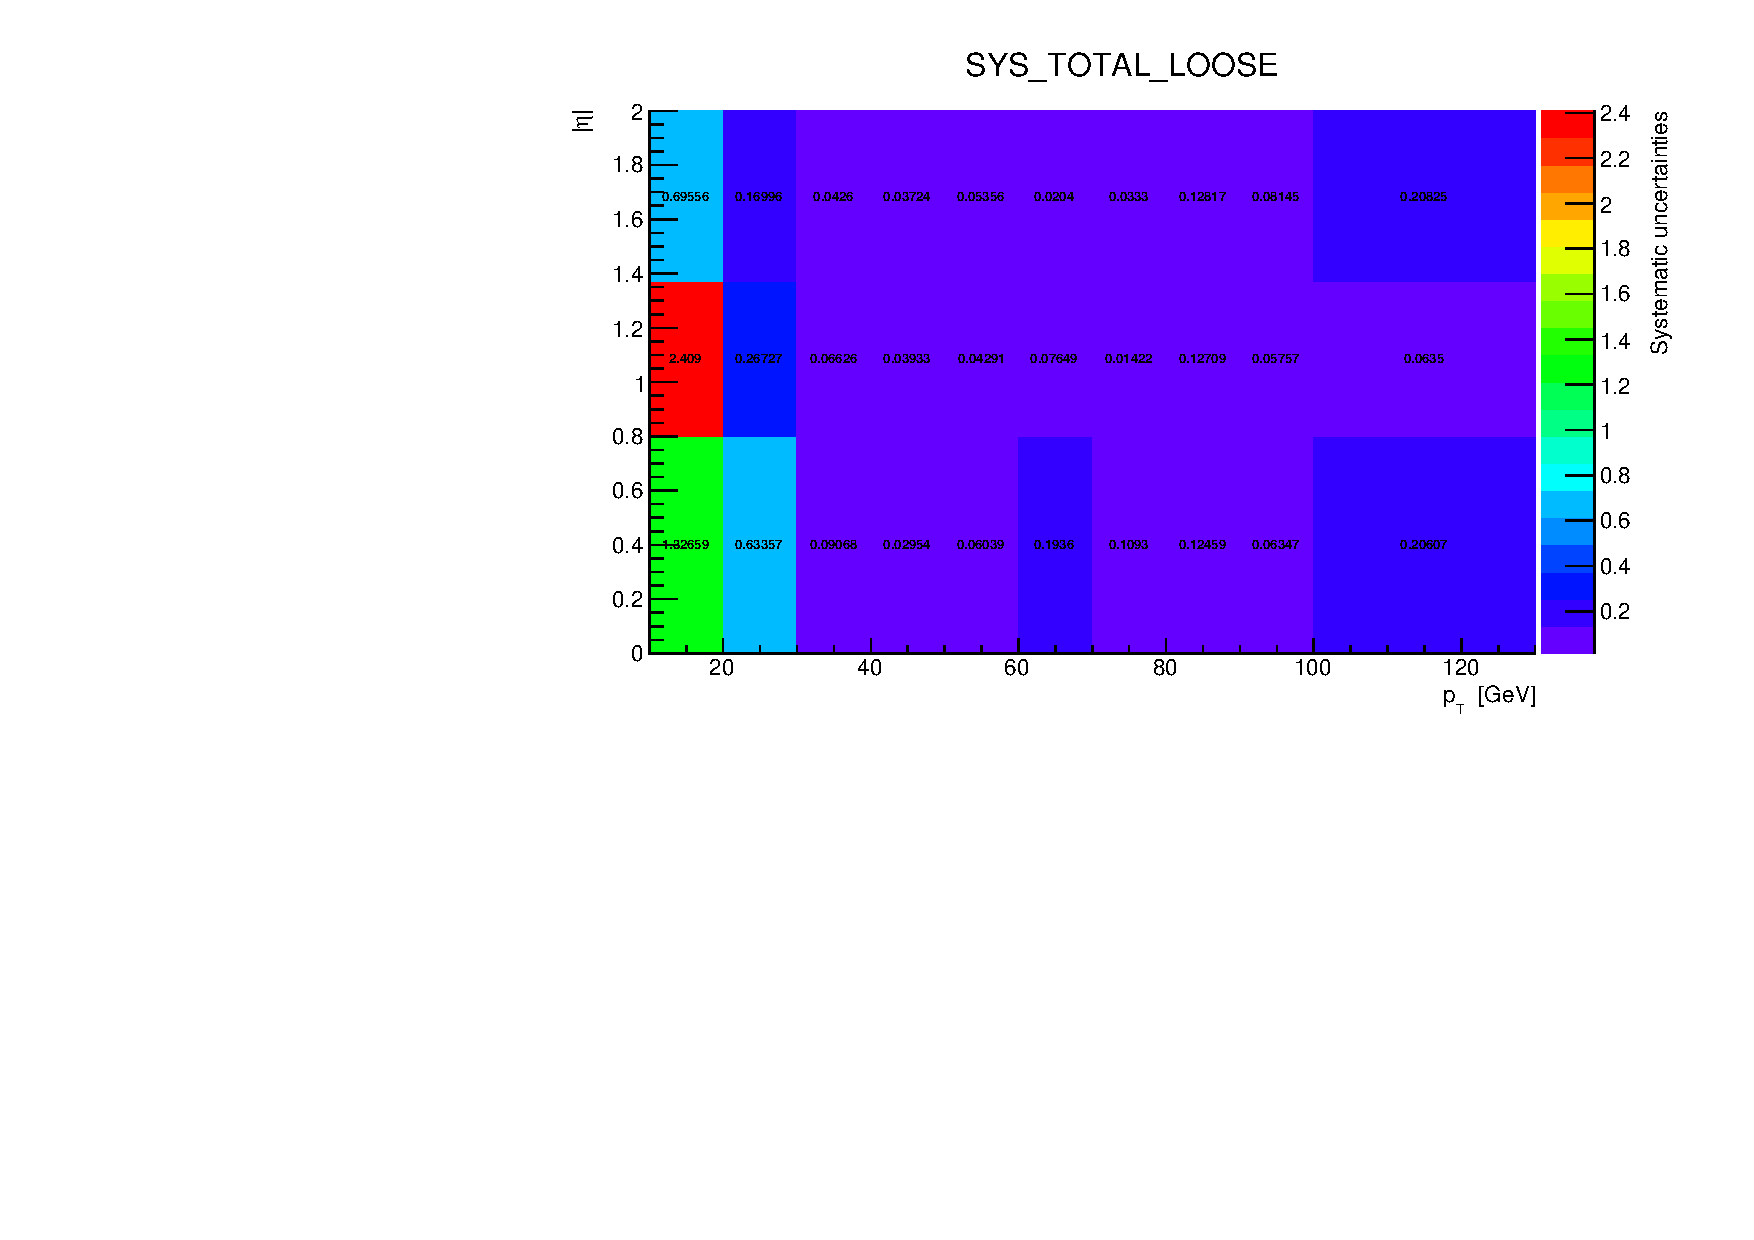
\includegraphics[width=0.65\textwidth]{FIGURES/BKG/chargeFlip/2D_histo_SYS_TOTAL_LOOSE.pdf}
\caption{\label{fig:CFsysTot} Total systematic uncertainties evaluated in each bins by taking the largest deviation coming from the comparison of different configurations in background subtraction method (in data) for electrons satisfying the signal requirements on the upper plot and for electrons failing the signal requirements on the lower plot.}
\end{figure}
